\documentclass[11pt]{dblab-thesis}

\usepackage{amsmath}
\usepackage{amssymb}
\usepackage{mathabx}
\usepackage{algpseudocode}
\usepackage{algorithm}
\usepackage{bbm}
\usepackage{graphicx}
\usepackage{multirow}
\usepackage{fontspec}
\usepackage{wasysym}
\usepackage{epsfig}
\usepackage{latexsym}
\usepackage{index}
\usepackage{forest}
\usepackage{color}
\usepackage{url}
\usepackage{hyperref}
{\renewcommand{\bibname}{References}} 
\usepackage[style=numeric,sorting=none]{biblatex}
\setmainfont{CMU Serif}
\setsansfont{CMU Sans Serif}
\newfontfamily{\greekfont}{CMU Serif}
\newfontfamily{\greekfontsf}{CMU Sans Serif}

\addbibresource{references.bib}  

\usepackage{nomencl}

\makenomenclature
\renewcommand{\nomname}{Πίνακας Ακρωνυμίων}
\renewcommand{\nompreamble}{Παρακάτω βρίσκεται η λίστα εννοιών που συναντιούνται συχνά στο κείμενο.}
\renewcommand{\listalgorithmname}{Αλγόριθμοι}
\renewcommand\UrlFont{\ttfamilylatin}
\floatname{algorithm}{Αλγόριθμος}

\definecolor{SeaGreen}{HTML}{2E8B57}
\definecolor{myGreen}{HTML}{66CC00}
\definecolor{Maroon}{HTML}{800000}
\definecolor{myGrey}{HTML}{A0A0A0}
\usepackage[nottoc]{tocbibind}

\title{Μετάδοση γνώσης βαθιών συνελικτικών νευρωνικών δικτύων για εντοπισμό αντικειμένων σε ενσωματωμένα συστήματα πραγματικού χρόνου}
\author{Ιωάννης Αθανασιάδης}
\supervisor{Λουκάς Πέτρου}
\TRnumber{ΕΣΒΓΔ-ΔΙΠΛ-2003-07}
\epitropiF{Γεώργιος Χασάπης}
\epitropiS{Ανδρέας Συμεωνίδης}


\DeclareMathAlphabet{\pazocal}{OMS}{zplm}{m}{n}
\DeclareRobustCommand{\bbone}{\text{\usefont{U}{bbold}{m}{n}1}}
\DeclareMathOperator{\EX}{\mathbb{E}}% expected value

\definecolor{LstItemCol}{HTML}{3333FF}


\begin{document}

\maketitle

\mainmatter
\begin{acknowledgements}
Θα ήθελα να ευχαριστήσω θερμά τους ανθρώπους που συνέβαλλαν ενεργά στη διεκπεραίωση αυτής της διπλωματικής. Τον επιβλέποντα καθηγητή μου κ. Λουκά Πέτρου για την εμπιστοσύνη που μου έδειξε και την στήριξή του καθ᾽ όλη τη διάρκεια της συνεργασίας μας όπως και τον επιβλέποντα διδακτορικό Υπ. Δρ. Παναγιώτη Μουσουλιώτη για την καθημερινή υποστήριξή του και τις συμβουλές του σε όλα τα στάδια της διπλωματικής. 

Θα ήθελα επίσης να ευχαριστήσω τον Υπ. Δρ. Κωνσταντίνο Παναγιώτου για τη πολύτιμη βοήθειά του και τις συμβουλές του στο πρακτικό κομμάτι της διπλωματικής όπως και τον Μεταδιδακτορικό Ερευνητή του τμήματος Εμμανουήλ Τσαρδούλια. 

Δε θα μπορούσα να μην ευχαριστήσω τον κ. καθηγητή Πιτσιάνη Νικόλαο για τη διαμόρφωση του τρόπου σκέψης μου όσον αφορά την παραλληλοποίηση και την αποδοτικότητα των αλγορίθμων, όπως και τους δασκάλους μου Αραμπατζή Γεώργιο και Δρ. Τιάκα Ελευθέριο.

Το θερμότερο Ευχαριστώ το οφείλω στους γονείς μου Στυλιανό και Παρασκευή και στα αδέρφια μου Παναγιώτη και Ανέστη στους οποίους στηρίχθηκα τόσο στην εκπόνηση αυτής της διπλωματικής όσο και στις σπουδές μου. Τέλος, είμαι ευγνώμων σε συγγενείς, φίλους και γνωστούς για την όποια συνεισφορά τους τόσο στην προσωπική όσο και στην επαγγελματική μου πορεία.

\end{acknowledgements}

\begin{abstract}
Στην παρούσα διπλωματική εργασία μελετήθηκε η τεχνική της μετάδοσης γνώσης στα συνελικτικά δίκτυα εντοπισμού αντικειμένων πραγματικού χρόνου. Αναλυτικότερα, εξετάζεται η γενικότητα ήδη γνωστών πειραμάτων απλών συνελικτικών νευρωνικών δικτύων στα δίκτυα εντοπισμού αντικειμένων πραγματικού χρόνου και κατά πόσο το φαινόμενο της συν-προσαρμογής είναι έντονο σε αυτά. Για το σκοπό των πειραμάτων υλοποιήθηκε εξ-αρχής η εκπαίδευση του νευρωνικού δικτύου SqueezeDet με ταχύτερη ροή και επεξεργασία δεδομένων δίνοντας συνολική επιτάχυνση $1.8$ φορές με τη κατασκευή ενός καινούριου και προτεινόμενου αλγορίθμου. Αρχικά, εξετάζονται τα πιο διαδεδομένα δίκτυα εντοπισμού αντικειμένων και οι βασικές αρχές σχεδίασής τους. Έπειτα, γίνεται μία ανασκόπηση των τεχνικών μετάδοσης γνώσης από όπου προκύπτουν και οι τελικοί πειραματισμοί μεταφερσιμότητας παραμέτρων του δικτύου SqueezeDet, μαζί με τη μελέτη του φαινομένου της συν-προσαρμογής. Οι πειραματισμοί αυτοί δείχνουν κυρίως κατά πόσο εύθραυστα μπορεί να είναι τα επίπεδα ενός νευρωνικού δικτύου στο φαινόμενο της συν-προσαρμογής. Επιπρόσθετα, παρουσιάζεται η βασική μεθοδολογία σχεδίασης του ταχύτερου τρόπου εκπαίδευσης μαζί με την έκθεση ενός καινούριου παραλλήλου αλγορίθμου αντιστοίχησης περιοχών ενδιαφέροντος και οι λεπτομέρειες υλικού και λογισμικού της υλοποίησης. Τέλος, μέσα από τα παραδείγματα μη επιτυχημένων μετεκπαιδεύσεων δίνονται οδηγίες για τους τρόπους με τους οποίους μπορεί να επιτευχθεί μία πετυχημένη μετεκπαίδευση καθώς και οι αρχικές συνθήκες οι οποίες θα πρέπει να ισχύουν πριν τη μετεκπαίδευση.

   \begin{keywords}
   Τεχνητή νοημοσύνη, Μηχανική μάθηση, Βαθιά μηχανική μάθηση, Υπολογιστική τεχνητή νοημοσύνη, Μετάδοση γνώσης, Νευρωνικά δίκτυα, Συνελικτικά νευρωνικά δίκτυα, Νευρωνικά δίκτυα εντοπισμού αντικειμένων, Ενσωματωμένα συστήματα, Παραλληλοποίηση αλγορίθμων
   \end{keywords}
\end{abstract}



\begin{abstracteng}
This thesis examines the transfer learning technique of real time convolutional neural networks for detection in embedded systems. More specifically, the generality of convolutional neural network experiments for transferability is studied in the case of object detection tasks. The experiments concluded for this tasks using real time neural networks lacks the study of co-adaptation which is a well studied phenomenon in recognition tasks for non-real time neural networks. For these experimentations a new training implementation of the SqueezeDet neural network is proposed with faster pipeline and data processing, achieving $1.8$ times total acceleration comparing to the initial implementation. This achievement is a result of a new parallel algorithm for matching regions of interest between the ground truth and the predicted ones. First, there is a mention to the essential detection convolutional neural networks that compose the state of the art and their design insights. Afterwards, a review of the transfer learning techniques follows, where the final experiment of the SqueezeDet weights transferability is derived, along with the study of co-adaptation. The experiments indicate the fragility of a neural network to co-adaptation. Furthermore, a key methodology for faster detection network training is presented and the parallel algorithm for matching the regions of interest is analyzed. Accompanying the speedup representation, the details of software structure and hardware are provided. At last, through failed examples of transfer learning there are recommendations about avoiding common mistakes and the required initial conditions for a successful transfer learning.


  \begin{keywordseng}
  Artificial intelligence, Machine learning, Deep learning, Computational artificial intelligence, Transfer learning, Neural networks, Convolutional neural networks, Detection neural networks, Embedded systems, Algorithm parallelization
  \end{keywordseng}

\end{abstracteng}



\tableofcontents
\listoffigures
\listoftables
\clearpage
\nomenclature{CNN}{Convolutional Neural Network, συνελεκτικό Νευρωνικό Δίκτυο}
\nomenclature{layer}{Επίπεδο του νευρωνικού δικτύου}
\nomenclature{Frame}{Καρέ}
\nomenclature{NMS}{Non Maximum Suppresion. Αλγόριθμος ο οποίος αν δύο περιβλήματα τέμνονται, τότε κρατάει μόνο αυτό με το μεγαλύτερο σκορ}
\nomenclature{RoI}{Region of Interest}
\nomenclature{mAP}{medium Average Precision. Μεσαία μέση ακρίβεια}
\nomenclature{ReLU}{Rectified Linear Unit. Πρόκειται για την μη γραμμική συνάρτηση ενεργοποίησης $ f(x) = max(0,x) $}
\nomenclature{TL}{Transfer Learning. Μετάδοση γνώσης}
\nomenclature{MTL}{Multi-Task Learning. Μάθηση πολλών έργων ταυτοχρόνως}
\nomenclature{GPU}{Graphics Processing Unit}
\nomenclature{CPU}{Central Processing Unit}
\nomenclature{RAM}{Random Access Memory}
\nomenclature{DL}{Deep Learning, Βαθιά Μηχανική Μάθηση}
\nomenclature{RL}{Reinforcement Learning, Ενισχυόμενη Μάθηση}
\nomenclature{GAN}{Generative Adversarial Network}
\nomenclature{SDP}{SemiDefinite Programming}
\nomenclature{PCA}{Principal Component Analysis}
\nomenclature{AUC}{Area Under the Curve}
\nomenclature{IOU}{Intersection Over Union. Μέτρο σύγκρισης επικάλυψης δύο ορθογωνίων κουτιών.}
\printnomenclature
\clearpage


\chapter{Εισαγωγή}
Η Τεχνητή Νοημοσύνη είναι ο κλάδος/τομέας της επιστήμης της πληροφορικής, που ασχολείται με την σχεδίαση και κατασκευή ευφυών συστημάτων, δηλαδή συστημάτων που διαθέτουν χαρακτηριστικά που σχετίζονται με την ανθρώπινη νοημοσύνη και συμπεριφορά. Ο πιο ισχυρός υπολογιστής που γνωρίζει ο άνθρωπος μέχρι στιγμής είναι ο ίδιος ο εγκέφαλός του(όπως βέβαια και οι εγκέφαλοι άλλων ζώων). Αυτός για να φτάσει στο σημείο να χαίρει της τωρινής υπολογιστικής του ικανότητας χρειάστηκε εκατομμύρια χρόνια βιολογικής εξέλιξης. Ακόμα και με αυτή την υπολογιστική ικανότητα που διαθέτει συνεχίζει να χρησιμοποιεί τη τεχνική μετάδοσης γνώσης, παρά τα χρόνια εξέλιξής του. Αυτό σύμφωνα με τη δαρβινική θεωρία \cite{74} τη φυσικής επιλογής, δείχνει πως ήταν μία βελτιστοποίηση στη λειτουργία του (δεν ισχυρίζεται η τελειότητα αυτού) η οποία δοκιμάστηκε και επέζησε μέχρι στιγμής.  

Ως εκ τούτου, ο σχεδιασμός αλγορίθμων και μοντέλων που εκπαιδεύονται μέσω της μετάδοσης γνώσης είναι μία αρκετά δοκιμασμένη επιλογή και μία αρκετά δικαιολογημένη απόφαση. Ωστόσο, έχοντας πάλι ως παράδειγμα τον εγκέφαλο, τα νευρωνικά δίκτυα εντοπισμού αντικειμένων θα έπρεπε να απαιτούν λιγότερες παραμέτρους και να επεξεργάζονται την είσοδό τους σε πραγματικό χρόνο (τουλάχιστον 24 καρέ /δευτερόλεπτο). Η τελευταία αυτή απαίτηση σε συνδυασμό με την προηγούμενη οδηγούν στη διαμόρφωση του προβλήματος που περιγράφεται παρακάτω.

Επιπλέον, η μετάδοση γνώσης είναι ένα από τα εργαλεία που είναι στενά συνδεδεμένο με την έννοια της Γενικής Τεχνητής νοημοσύνης(Artificial General Intelligence). Αυτό συμβαίνει γιατί μοντελοποιείται ένα πολύ σημαντικό κομμάτι της διαδικασίας του εγκεφάλου: η ίδια η μάθηση.

Ένας σημαντικός τομέας που ωθεί τα σύγχρονα επιτεύγματα στη τεχνητή νοημοσύνη είναι η εμφάνιση και εξέλιξη του κλάδου της Βαθιάς Μηχανικής Μάθησης (Deep learning - DL).Η χρήση τεχνικών βαθιάς μάθησης στην επίλυση προβλημάτων Μηχανικής Όρασης, έχει κατορθώσει να αντιμετωπίσει περίπλοκα προβλήματα τα οποία μέχρι και πριν από λίγα χρόνια θεωρείτο ακατόρθωτο να λυθούν. Ακόμα και η χρήση της DL σε ενσωματωμένα συστήματα με μικρή μνήμη και απαιτήσεις ταχύτατης επεξεργασίας δίνει καλύτερα αποτελέσματα από ότι άλλοι αλγόριθμοι.

Σήμερα, το γενικότερο πρόβλημα της ταυτόχρονης αναγνώρισης και εντοπισμού αντικειμένων σε εικόνες χρησιμοποιεί εκτεταμένα Νευρωνικά Δίκτυα Συνέλιξης (Convolutional Neural Networks - CNNs). Η εκπαίδευση και η επανεκπαίδευση αυτών έχει επισημανθεί ότι ωφελείται αρκετά από τη χρήση τεχνικών μετάδοση γνώσης \cite{55}. Σε αυτό παίζουν ρόλο και άλλοι οικονομοτεχνικοί λόγοι όπως το μέγεθος των διαθέσιμων δεδομένων. Σε συνδυασμό όλων των παραπάνω η εργασία καλείται να δώσει κάποιες παρατηρήσεις προς την επίλυση του παρακάτω προβλήματος.

\section{Περιγραφή του Προβλήματος}
Παρόλο που τα νευρωνικά δίκτυα εντοπισμού αντικειμένων από εικόνες έχουν φτάσει στο σημείο να έχουν ικανοποιητική ακρίβεια και να εκτελούνται σε ενσωματωμένα συστήματα, δεν έχουν μελετηθεί όλες οι διαφορές τους και οι σχέσεις τους με αυτά που έχουν μεγάλο αριθμό παραμέτρων και εκτελούνται με μεγαλύτερη απαίτηση ισχύος. Η κύρια μελέτη αυτών των συστημάτων έγκειται στον χρόνο εκτέλεσης, την ακρίβεια και πρόσφατα τη μνήμη \cite{1} και την απαίτηση σε ισχύ. Ένα μεγάλο κεφάλαιο στην κατεύθυνση της έρευνας για τα νευρωνικά δίκτυα που μπορούν να εκτελούνται σε ενσωματωμένα συστήματα είναι η μετάδοση γνώσης.

Είναι σημαντικό για παράδειγμα ένα ρομπότ να μπορεί να χρησιμοποιήσει την προηγούμενα επεξεργασμένη (και μη) πληροφορία που διαθέτει για την ανάκτηση και την επεξεργασία καινούριας. Κατά αυτό τον τρόπο μειώνεται ο χρόνος εκπαίδευσής του σε μία καινούρια εργασία. Ωστόσο, είναι θεμιτό οι ενσωματωμένες συσκευές να είναι όσο πιο “ελκυστικές” γίνεται και συνήθως αρκετά μικρότερες σε μέγεθος από μία συστοιχία υπολογιστών \cite{70, 71}, ανάλογα με την εργασία που επιθυμούμε να εκτελέσουν. Αυτό, έχει ως αποτέλεσμα να μην μπορούν να τοποθετηθούν ογκώδη, άρα με μεγάλη επεξεργαστική ισχύ, υπολογιστικά συστήματα στα ενσωματωμένα συστήματα.

Ήδη η μετάδοση γνώσης χρησιμοποιείται συνεχώς σε προβλήματα ενισχυόμενης μάθησης(RL) \cite{72, 73}, ώστε να μπορεί το μοντέλο ενός πράκτορα να μεταφερθεί από την προσομοίωση στην πραγματικότητα. Το ίδιο απαιτείται και στην περίπτωση της τεχνητής όρασης με σκοπό την εξοικονόμηση δεδομένων, την ταχύτερη και την αποτελεσματικότερη εκπαίδευση. Το πρόβλημα είναι πως δεν έχουν γίνει πειραματισμοί και μελέτες για την καταγραφή της συμπεριφοράς των νευρωνικών δικτύων εντοπισμού αντικειμένων ενσωματωμένων συστημάτων ως προς τη μετάδοση γνώσης.

\section{Σκοπός-Συνεισφορά της Διπλωματικής Εργασίας}
Η παρούσα διπλωματική εργασία μελετά την επαναχρησιμοποίηση νευρωνικών δικτύων συνέλιξης (CNN) σε εφαρμογές ταυτόχρονης αναγνώρισης και εντοπισμού αντικειμένων (object recognition and localization - object detection) σε εικόνες.

Βασικός σκοπός είναι η μεταφορά πληροφορίας μοντέλων CNN από προηγούμενες εφαρμογές, διατηρώντας κατά το δυνατόν σταθερή την αρχιτεκτονική ώστε να επιτρέπεται συνεχώς η εφαρμογή τους σε προβλήματα πραγματικού χρόνου. Μία ακόμα απαίτηση είναι η ελάχιστη μνήμη του αλγορίθμου, προκειμένου να είναι δυνατή η εκτέλεσή του από όσο περισσότερες ενσωματωμένες συσκευές. Επίσης, ζητείται η κατά το δυνατόν υψηλότερη ακρίβεια του μοντέλου μετά από την εκπαίδευση του και μεταφορά γνώσης. Τέλος, απαιτείται η κατά το δυνατόν γρηγορότερη επανεκπαίδευσή του. Όλες αυτές οι απαιτήσεις εξετάζονται κατά το πόσο είναι εφικτές και τι περιορισμούς προϋποθέτουν. Η εξέταση αυτή γίνεται πρώτη φορά μέχρις στιγμής καθότι η μετάδοση γνώσης είναι αρκετά καινούρια τεχνική στο τομέα της τεχνητής νοημοσύνης όπως και τα νευρωνικά δίκτυα εντοπισμού πραγματικού χρόνου.

Επίσης, παρουσιάζεται ένας πιο γρήγορος αλγόριθμος για την εκπαίδευση του νευρωνικού δικτύου εντοπισμού \textit{SqueezeDet}, όπως και η εφαρμογή ενός νέου τρόπου βελτιστοποίησης υπερπαραμέτρων των νευρωνικών δικτύων. Τέλος, γίνεται και μία πειραματική αναφορά στην πλαστικότητα των νευρώνων των δικτύων εντοπισμού αντικειμένων για ενσωματωμένα συστήματα.

\section{Διάρθρωση της αναφοράς}
Η διάρθρωση της παρούσας διπλωματικής εργασίας είναι η εξής:

\begin{itemize}
    \item \textbf{Κεφάλαιο \ref{chapter:neuralNets}} Περιγράφονται τα σημαντικότερα νευρωνικά δίκτυα εντοπισμού αντικειμένων σε εικόνα. Γίνεται αναφορά στη δυνατότητα εκτέλεσής τους από ενσωματωμένες συσκευές και προς το σκοπό αυτό γίνονται και μετρήσεις.
    \item \textbf{Κεφάλαιο \ref{chapter:tl}} Δίνονται οι ορισμοί που αφορούν τη μετάδοση γνώσης. Αναφέρονται παραδείγματα και τεχνικές μετάδοσης γνώσης, όπως επίσης και το θεωρητικό υπόβαθρο για το μετέπειτα πειραματισμό. 
    \item \textbf{Κεφάλαιο \ref{chapter:experiments}} Παρουσιάζονται τα πειράματα από την περιγραφή τους, τα αποτελέσματά τους και τέλος τα συμπεράσματα που προέρχονται από αυτά.
    \item \textbf{Κεφάλαιο \ref{chapter:accel_SqueezeDet}} Παρουσιάζονται οι τρόποι και οι αλγόριθμοι που συντέλεσαν στην επιτάχυνση της εκπαίδευσης του νευρωνικού δικτύου \textit{SqueezeDet}.    
    \item \textbf{Κεφάλαιο \ref{chapter:architecture}} Επιγραμματική περιγραφή της υλοποίησης των πειραμάτων όσον αφορά το υλικό και το λογισμικό που χρησιμοποιήθηκε.
    \item \textbf{Κεφάλαιο \ref{chapter:futures}} Αναφέρονται τα προβλήματα που προέκυψαν και προτείνονται
    θέματα για μελλοντική μελέτη, αλλαγές και επεκτάσεις.
\end{itemize} % started
\chapter{Νευρωνικά Δίκτυα για Εντοπισμό Αντικειμένων}%
\label{chapter:neuralNets}
\section{Εισαγωγή}
Τα τελευταία χρόνια έχει προταθεί ένας μεγάλος αριθμός νευρωνικών δικτύων για τον εντοπισμό αντικειμένων από εικόνες. Η εισαγωγή της έννοιας του CNN, όπου πρόκειται για νευρωνικό δίκτυο το οποίο έχει επίπεδα που εκτελούν συνελίξεις για την αναγνώριση χειρόγραφων αριθμών είχε ήδη προταθεί το 1998 \cite{36} και το 2006 \cite{35}. Ωστόσο, λόγω υψηλής απαίτησης σε υπολογιστική ισχύ δεν προτεινόταν η χρήση τους στην επίλυση προβλημάτων αναγνώρισης αντικειμένων ή εντοπισμό. Η αλλαγή της πορείας έγινε το 2012, όταν προτάθηκε το AlexNet \cite{20} το οποίο είναι ένα νευρωνικό δίκτυο πολλών επιπέδων (deep) το οποίο έχει επίπεδα συνελίσουν την είσοδό τους με τα βάρη τους (convolutional). Με αυτό παρουσιάζονται και οι δύο συγκυρίες που έδωσαν ώθηση στη βαθιά μηχανική μάθηση - τα σύνολα δεδομένων (π.χ. ImageNet) και η υπολογιστική ισχύς των GPU (η εκπαίδευση είναι πλέον εφικτή σε σχετικά μικρό χρόνο). Από τότε και έπειτα άρχισε η χρήση και η δημιουργία καινούριων CNN για προβλήματα που εμπεριέχουν την αναγνώριση και τον εντοπισμό αντικειμένων. Τα δίκτυα που προτάθηκαν το δεύτερο μισό του 2017 και μόνο για την αναγνώριση/εντοπισμό αντικειμένων ξεπερνούν τα δέκα. Επιπλέον η απαίτηση χρήση τους σε πραγματικού χρόνου εφαρμογές και σε ενσωματωμένα συστήματα έδωσε μια άλλη οπτική ανάπτυξής τους. Σε αυτό το κεφάλαιο αναλύονται τα σημαντικότερα δίκτυα που αποτελούν ορόσημα για την χρήση των νευρωνικών σε ενσωματωμένες συσκευές.

% Template of a new CNN-net
% Title: A new net 
% Contents:
% 1. When was proposed
% 2. What makes it special for detection
% 3. Architecture descritpion
% 4. Training & Retraining
% 5. Accuracy
% 6. Speed
% 7. Memory
% 8. Energy consumption
% 9.”Is it good for embedded systems?”

\section{SqueezeDet-Net \cite{1} \cite{2}}
Τα δίκτυα αυτά προτάθηκαν από ερευνητές του πανεπιστημίου του Berkeley και της εταιρίας Deepscale ως μια λύση για το πρόβλημα του μεγάλου αριθμού παραμέτρων ενός νευρωνικού δικτύου για εντοπισμό αντικειμένων. Το SqueezeΝet ουσιαστικά εμπεριέχεται στο SqueezeDet ως ένα από τα επίπεδά του. Και τα δύο προτάθηκαν για επίλυση προβλημάτων που αφορούν την αυτοκινητοβιομηχανία. Η μείωση του αριθμού των παραμέτρων κάνει εφικτή την αναγνώριση αντικειμένων σε πραγματικό χρόνο και επιτυγχάνει μεγαλύτερη ενεργειακή αποδοτικότητα. Σε σύγκριση με το AlexNet\cite{20}, επιτυγχάνει την ίδια ακρίβεια με 50x μικρότερο μέγεθος παραμέτρων. Η είσοδος που δέχεται είναι το ήδη επεξεργασμένο αποτέλεσμα του SqueezeNet.

\begin{figure}[H]
\centering
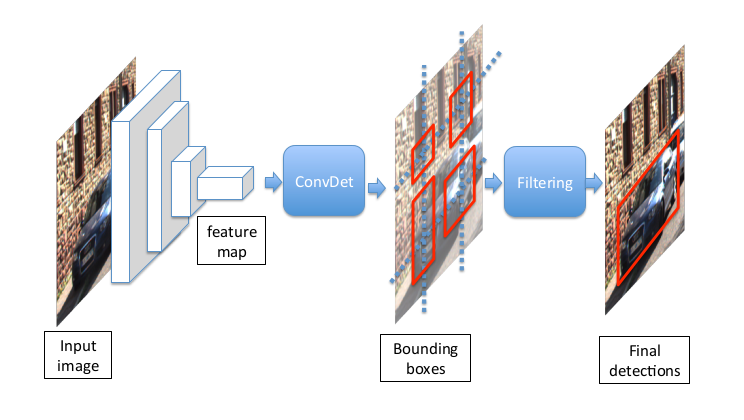
\includegraphics[width = \textwidth]{figures/SqueezeNetDet/SqueezeDet_architecture.png}
\caption[Αρχιτεκτονική SqueezeDet]{Η σειρά επεξεργασίας του SqueezeDet για εντοπισμό αντικειμένων. Ένα CNN π.χ. SqueezeNet εξάγει χαρακτηριστικά από την εικόνα εισόδου και τα δίνει ως είσοδο στο επίπεδο ConvDet. Με τη σειρά του, το επίπεδο ConvDet υπολογίζει τα ορθογώνια περιβλήματα γύρω από τα ομοιόμορφα κατανεμημένα $ W\times H$ κέντρα των πιθανών αντικειμένων. Κάθε ορθογώνιο περίβλημα σχετίζεται με $1$ σκορ εμπιστοσύνης και $C$ υπό συνθήκη πιθανότητες. Κατά το επίπεδο \textit{Filtering} κρατούνται τα $N$ περιβλήματα με τα κυρίαρχα σκορ εμπιστοσύνης και χρησιμοποιούνται αλγόριθμοι \textit{NMS} για τη λήψη των τελικά εντοπισμένων αντικειμένων.}
\label{fig:SqueezeDet_architecture}
\end{figure}


Η αρχιτεκτονική του SqueezeDet, του επιτρέπει να προτείνει την ορθογώνια περιοχή μέσα στην οποία εντοπίζει ένα αντικείμενο σε μία εικόνα αλλά και να το κατηγοριοποιεί ταυτόχρονα. Ουσιαστικά αποτελείται από ένα επίπεδο συνελίξεων το οποίο προτείνει τις περιοχές ύπαρξης αντικειμένων και ένα NMS (Non-Maximum Suppression) φίλτρο για υπολογισμό της πιθανότητας ύπαρξης κάποιου αντικειμένου στις προτεινόμενες περιοχές. Το φίλτρο εφαρμόζεται σε όλη την έξοδο του ConvNet και η πιθανότητα υπολογίζεται από τον τύπο:
$$ max \{ Pr\left(class_C| Object\right)\} * Pr(Object) * IOU^{pred}_{truth} $$

To SqueezeNet με τη σειρά του αποτελεί ιδανική υλοποίηση του επιπέδου συνελίξεων του SqueezeDet γιατί στοχεύει στον μικρό αριθμό παραμέτρων. Επίσης, κατά τη σχεδίασή του δόθηκε περισσότερη έμφαση στον διανυσματικό χώρο των βαρών με δεδομένη ακρίβεια και όχι το ανάποδο. Αυτό ήταν που οδήγησε στις παρακάτω τρεις στρατηγικές για τη μείωση του αριθμού των παραμέτρων:

\begin{enumerate}
    \item Αντικατάσταση των $3\times3$ φίλτρων με $1\times1$.
    \item Μείωση του αριθμού καναλιών στα $3\times3$ φίλτρα, με χρήση επιπλέον επιπέδων (\textit{squeeze layers}).
    \item H υποδειγματοληψία γίνεται στα τελευταία layers του δικτύου.
\end{enumerate}

Με εφαρμογή αυτών των τριών στρατηγικών και με υλοποίηση της λογικής "Network in Network"\cite{75} των ResNet \cite{21} και GoogleNet \cite{24} το νευρωνικό αποτελείται από μικρότερες οντότητες, οι οποίες ονομάζονται \textit{fire modules}. Κάθε τέτοια οντότητα όπως φαίνεται στο Σχήμα \ref{fig:SqueezeNet_microarchitecture} ορίζεται από τις παραμέτρους:
\begin{itemize}
  \setlength\itemsep{0em}
    \item {$ s_{1 \times 1} $ ο αριθμός φίλτρων στο \textit{squeeze layer}}
    \item {$ e_{1 \times 1} $ o αριθμός $ 1\times1 $ φίλτρων στο \textit{expand layer}}
    \item {$ e_{3 \times 3} $  o αριθμός $ 3\times3 $ φίλτρων στο \textit{expand layer}}
\end{itemize}

Προκειμένου να επιτευχθεί η στρατηγική 2 απαιτείται $s_{1\times1} < (e_{1\times1} + e_{3\times3})$. Έπειτα ολόκληρη η αρχιτεκτονική αποτυπώνεται καλύτερα στο Σχήμα \ref{fig:SqueezeNet_microarchitecture}. Επιπλέον %χρησιμοποιείται η τεχνική \textit{dropout} \cite{3} με ποσοστό 50\% και 
στην είσοδο των $3\times3$ φίλτρων γίνεται \textit{zero-padding} κατά $1$ εικονοστοιχείων στο σύνορο.

Η εκπαίδευση του δικτύου γίνεται με \textit{Stochastic Gradient Descent} χρησιμοποιώντας την ίδια συνάρτηση κόστους που χρησιμοποιεί το δίκτυο YOLO\cite{6}. Κατά την εκκίνηση το learning rate είναι 0.04, το οποίο μειώνεται κατά την πάροδο των εποχών. Στο τέλος της εκπαίδευσης μπορεί να εφαρμοστεί και η τεχνική Deep Compression στο SqueezeNet με την οποία χρησιμοποιώντας μόνο 0.66 ΜΒ επιτυγχάνεται ακρίβεια 80.3\% στα 6 bit στο σύνολο δεδομένων του ImageNet. Η συνάρτηση κόστους εκπαιδεύει και τα 2 επίπεδα της αρχιτεκτονικής:

% \begin{figure}[H]
% \centering
% 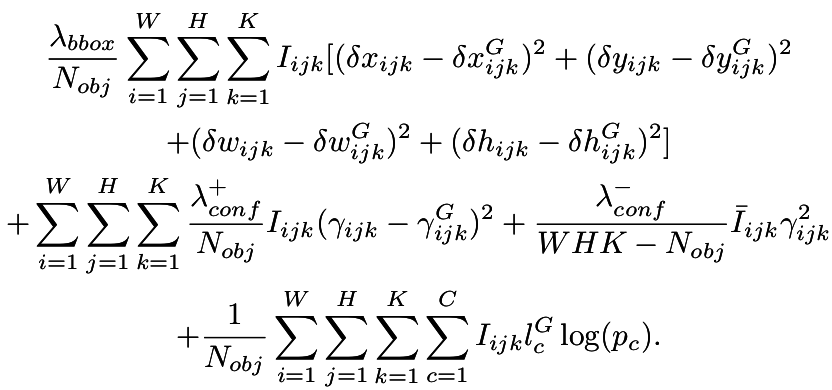
\includegraphics[width = \textwidth]{figures/SqueezeNetDet/SqueezeDet_lossFunction.png}
% \end{figure}

$$
\frac{\lambda_{bbox}}{N_{obj}} \sum_{i=1}^{W} \sum_{j=1}^{H} \sum_{k=1}^{K} I_{ijk} \left[(\delta\chi_{ijk} - \delta\chi_{ijk}^{G})^2 + ({\delta y}_{ijk} - {\delta y}_{ijk}^{G})^2 \right.
$$

$$
\left. + ({\delta w}_{ijk} - {\delta w}_{ijk}^{G})^2 + ({\delta h}_{ijk} - {\delta h}_{ijk}^{G})^2\right]
$$

$$
+ \sum_{i=1}^{W} \sum_{j=1}^{H} \sum_{k=1}^{K} \frac{\lambda_{conf}^{+}}{N_{obj}} I_{ijk} (\gamma_{ijk} - \gamma_{ijk}^G)^2 + \frac{\lambda_{conf}^{-}}{W H K - N_{obj}} \bar{I}_{ijk}\gamma_{ijk}^{2}
$$

$$
 + \frac{1}{N_{obj}} \sum_{i=1}^{W} \sum_{j=1}^{H} \sum_{k=1}^{K} \sum_{c=1}^{C} I_{ijk}l_{c}^{G}\log(p_c)
$$

Το πρώτο κομμάτι είναι για την εύρεση του περιβλήματος των αντικειμένων. Το σημείο $({\delta x}_{ijk}, {\delta y}_{ijk}, {\delta w}_{ijk}, {\delta h}_{ijk})$ αφορά τις σχετικές συντεταγμένες του πιθανού περιβλήματος ως προς το σημείο $(i,j)$. Το δεύτερο κομμάτι (η γραμμή με το δεύτερο τριπλό άθροισμα) αφορά την παλινδρόμηση για το σκορ εμπιστοσύνης. Έπειτα, το τρίτο κομμάτι αφορά την cross-entropy για κατηγοριοποίηση των αντικειμένων σε κλάσεις.
Η ακρίβεια του αλγορίθμου υπολογίστηκε πάνω στο σύνολο δεδομένων του KITTI και δίνεται με το κριτήριο (mAP) για τους πεζούς, τα αυτοκίνητα και τους ποδηλάτες.

\begin{tabular}{|*{10}{c|}} 
\hline
Μέθοδος & \multicolumn{3}{c|}{Car} & \multicolumn{3}{c|}{Cyclist} & \multicolumn{3}{c|}{Pedestrian}\\
\hline
SqueezeDet & 90.2 & 84.7 & 73.9 & 82.9 & 75.4 & 72.1 & 77.1 & 68.3 & 65.8 \\
SqueezeDet+ & 90.4 & 87.1 & 78.9 & 87.6 & 80.3 & 78.1 & 81.4 & 71.3 & 68.5 \\
\hline
\end{tabular}

\begin{tabular}{|*{3}{c|}}
\hline
Μέθοδος & Model size (MB) & mAP \\
\hline
SqueezeDet & 7.9 & 76.7\\
SqueezeDet+ & 26.8 & 80.4\\
\hline
\end{tabular}

Η απαίτηση μνήμης παρά τον παραπάνω πίνακα μπορεί να μειωθεί περαιτέρω. Με τη χρήση τεχνικών συμπίεσης και επηρεάζοντας τις υπερπαραμέτρους επιτυγχάνεται παραπάνω από $95\times$ συμπίεση κρατώντας την ίδια ευαισθησία. Ταυτόχρονα κερδίζει σε ταχύτητα και κατανάλωση ενέργειας. Μπορεί να φτάσει έως και τα 57.2 FPS στο KITTI, ενώ η ενισχυμένη εκδοσή του (SqueezeDet+) τα 32.1 FPS. Ο μειωμένος αριθμός παραμέτρων οδηγεί σε λιγότερη προσπέλαση μνήμης και οπότε λιγότερη χρήση της DRAM. Αυτή με τη σειρά της οδηγεί σε χαμηλότερη κατανάλωση ενέργειας είναι από 1.4 έως 4.0J/frame στο ΚΙΤΤΙ ανάλογα την έκδοση του SqueezeDet.

Ο χρόνος εκτέλεσης μειώνεται και αυτός με τη μείωση του αριθμού των παραμέτρων του δικτύου. Αν και στο ίδιο το έγγραφο που πρωτοπαρουσιάζεται το δίκτυο δε γίνεται λόγος για αυτό, η ενέργεια που καταγράφεται σε ενσωματωμένες συσκευές στο \cite{5}  είναι 26.37 J/frame στην πλατφόρμα του Nexus 5 για την εκτέλεση του SqueezeNet μόνο. Μάλιστα η παράλληλη υλοποίησή του οδηγεί σε ακόμα μικρότερη κατανάλωση ενέργειας. Για την ίδια πλατφόρμα έχει 249.47X λιγότερες ενεργειακές απαιτήσεις. Τέλος, η απαίτηση μνήμης, η κατανάλωση ενέργειας και η χρονική απόκριση του νευρωνικού, το χρήζουν κατάλληλο για ενσωματωμένα συστήματα.

\begin{figure}[H]
\centering
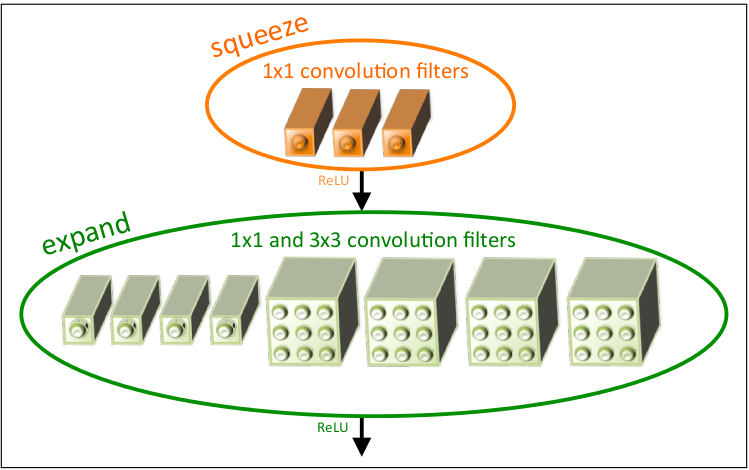
\includegraphics[width = \textwidth]{figures/SqueezeNetDet/SqueezeNet_microarchitecture.png}
\caption[Αρχιτεκτονική Fire module]{Μικροσκελής όψη της αρχιτεκτονικής SqueezeNet \cite{1}. Στην εικόνα φαίνεται το \textit{Fire module}, το οποίο είναι η βασική οντότητα όλου του SqueezeNet. Σε αυτό το παράδειγμα, $ s_{1x1} = 3, e_{1x1} = 4, e_{3x3} = 4$.}
\label{fig:SqueezeNet_microarchitecture}
\end{figure}

\begin{figure}[H]
\centering
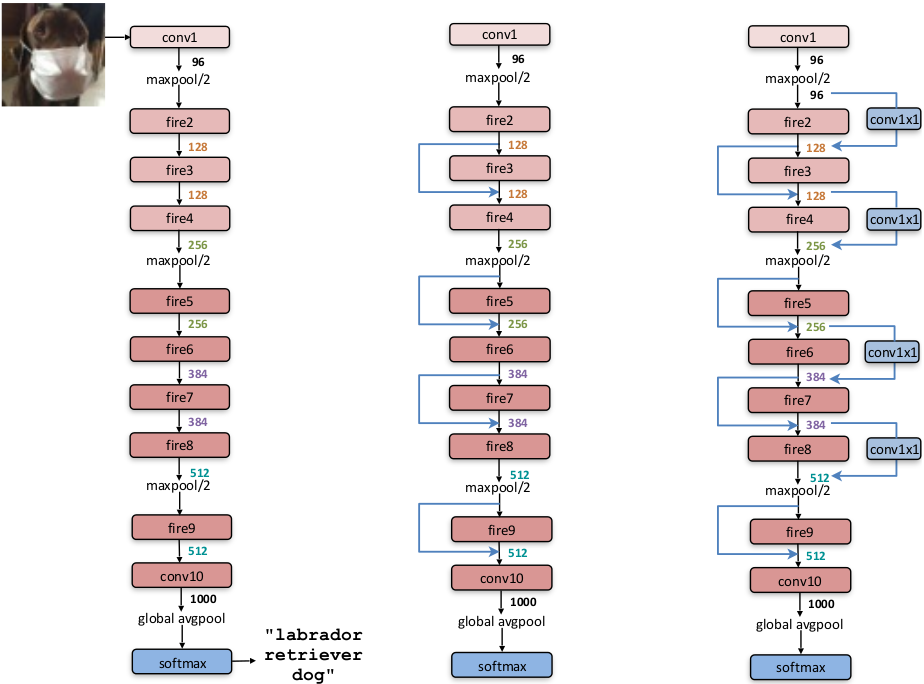
\includegraphics[width = \textwidth]{figures/SqueezeNetDet/SqueezeNet_macroarchitecture.png}
\caption[Αρχιτεκτονική SqueezeNet]{Μακροσκελής όψη της αρχιτεκτονικής SqueezeNet \cite{2}. Τα δίκτυα που παρουσιάζονται είναι τα: απλό SqueezeNet (αριστερά), SqueezeNet με απλό \text{bypass} (μέση), SqueezeNet με σύνθετο \text{bypass} (δεξιά). Η σύνδεση προηγουμένων επιπέδων με το επόμενο και όχι μόνο του αμέσως προηγούμενου ωφελεί την ακρίβεια του δικτύου.}
\label{fig:SqueezeNet_macroarchitecture}
\end{figure}



\section{YOLO\cite{6}}

Το δίκτυο αυτό προτάθηκε ως μια λύση για το πρόβλημα της πραγματικού χρόνου αναγνώρισης αντικειμένων διατηρώντας όσο το δυνατόν μεγαλύτερη μέση ακρίβεια. Χαρακτηρίζεται από το όνομά του \textit{You Only Look Once} που υποδηλώνει πως τόσο κατά τον εντοπισμό/αναγνώρισή όσο και κατά την εκπαίδευση, το δίκτυο λαμβάνει την εικόνα εισόδου μία φορά και δεν την επεξεργάζεται ξανά μετά την είσοδο κατά την εκτέλεση του. Οπότε, λαμβάνεται υπόψιν και η κατά το δυνατόν γρηγορότερη εκπαίδευση του. Οι ικανότητες του πέρα από την ταχύτητα και την ακρίβειά του είναι και ο ταυτόχρονος εντοπισμός πολλών διαφορετικών αντικειμένων σε μία εικόνα και η χωροθέτηση τους.

Αρχικά για την επιλογή της αρχιτεκτονικής οι συγγραφείς θεώρησαν πως η αναγνώριση αντικειμένων μπορεί να θεωρηθεί ως πρόβλημα απλής παλινδρόμησης. Επειδή η επεξεργασία εισόδου γίνεται μία φορά, η αρχιτεκτονική του νευρωνικού αποτελείται από επίπεδα συνέλιξης, υποδειγματοληψίας και από δύο ολικά συνδεδεμένα επίπεδα στο τέλος. Τα επίπεδα αυτά είναι συνδεδεμένα εν σειρά. H αναγνώριση της κλάσης του αντικειμένου αλλά και του περιβλήματος του γίνεται την ίδια χρονική στιγμή. Για αυτό το αποτέλεσμα του νευρωνικού είναι ένα πλέγμα $ S \times S $ κελιών που κάθε κελί χωρίζει ισόποσα την εικόνα. Επίσης προβλέπει $Β$ περιβλήματα αντικειμένων και για το κάθε ένα από αυτά ένα σκορ εμπιστοσύνης. Το σκορ εμπιστοσύνης δείχνει την πιθανότητα το περίβλημα περιέχει ένα αντικείμενο. Όλα τα περιβλήματα του δικτύου YOLO είναι ορθογώνια. Η πληροφορία που περιγράφει ένα περίβλημα είναι $ (x, y, w, h, \text{σκορ εμπιστοσύνης}) $
\begin{itemize}
  \setlength\itemsep{0em}
\item[] $(x,y)$: το κέντρο του περιβλήματος
\item[] $w =$ πλάτος ορθογωνίου / πλάτος εικόνας
\item[] $h =$ ύψος ορθογωνίου / ύψος εικόνας
\end{itemize}

Επιπλέον κάθε κελί έχει και $C$ πιθανότητες $ Pr{Class_i| Object},\ i=1,..,C $. Οπότε συνολικά η έξοδος του νευρωνικού είναι ένας τανυστής $S\times S\times(B\cdot5+C)$. Η αρχιτεκτονική του φαίνεται και αναλυτικά στο Σχήμα \ref{fig:YOLO_architecture}.

\begin{figure}[H]
\centering
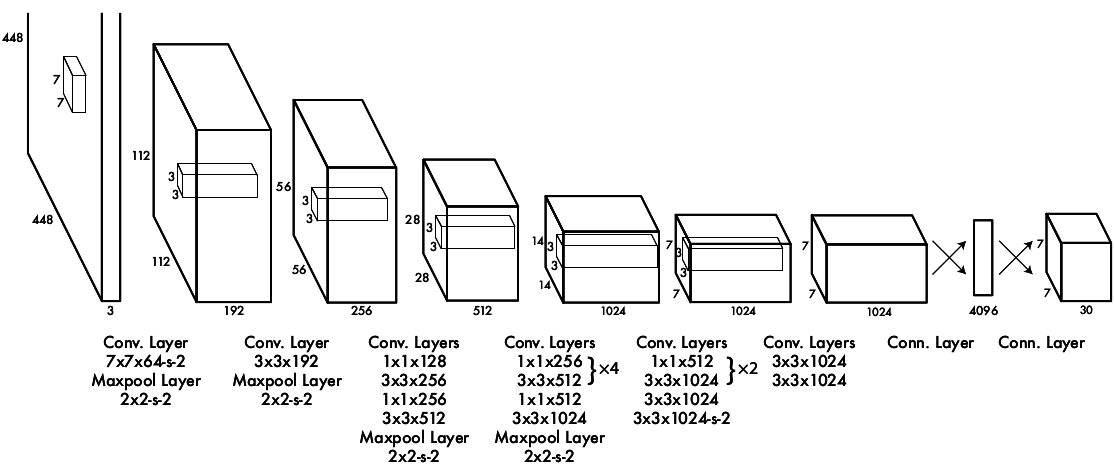
\includegraphics[width = \textwidth]{figures/YOLO/YOLO_architecture.png}
\caption[Αρχιτεκτονική YOLO]{Παράδειγμα της αρχιτεκτονικής YOLO \cite{6} για εικόνα εισόδου $224 \times 224$  όπου $S = 7, B = 2, C = 20 $. Το YOLO έχει 24 συνελεκτικά επίπεδα ακολουθούμενα από 2 ολικά συνδεδεμένα επίπεδα. Η χρήση $1 \times1 $ συνελεκτικών επιπέδων μπορεί να μειώσει τον χώρο των χαρακτηριστικών από τα προηγούμενα επίπεδα. Επίσης τα συνελεκτικά επίπεδα αρχικά εκπαιδεύονται στο ImageNet χρησιμοποιώντας τη μισή ανάλυση εικόνας ($224 \times 224$ εικόνα εισόδου) και μετά χρησιμοποιώντας τη διπλάσια για τον εντοπισμό αντικειμένων.}
\label{fig:YOLO_architecture}
\end{figure}

Ως συναρτήσεις ενεργοποίησης, αντί για τις πλέον διαδεδομένες \textit{ReLU} χρησιμοποιείται μια παραπλήσια μορφή: 

% \begin{equation}
$$
\phi(x) = \left\{ \begin{array}{cc}
    x, & x > 0 \\
    0.1 x, & \text{αλλιώς}
    \end{array}
    \right.
$$
% \end{equation}


Η εκπαίδευση γίνεται με κύριο σκοπό την βελτιστοποίηση του τετραγωνικού σφάλματος της εξόδου. Ως συνάρτηση απωλειών χρησιμοποιείται η συνάρτηση:

% \begin{figure}[H]
% \centering
% 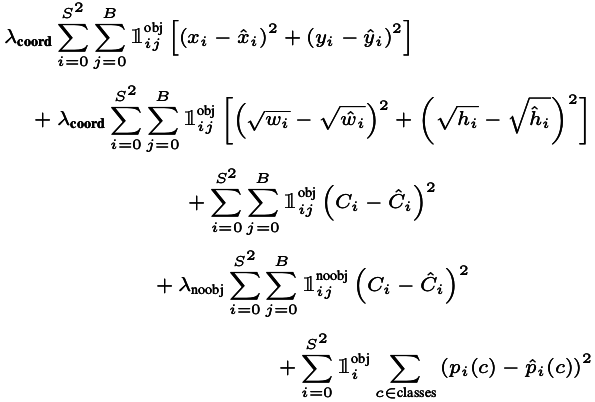
\includegraphics[width = 3in]{figures/YOLO/YOLO_lossFunction.png}
% \end{figure}
$$
\lambda_{coord} \sum_{i=0}^{S^2} \sum_{j=0}^{B} \mathbbm{1}_{ij}^{obj} \left[ (x_i-\hat{x_i})^2 + (y_i-\hat{y_i})^2\right]
$$
$$
   + \lambda_{coord} \sum_{i=0}^{S^2} \sum_{j=0}^{B} \mathbbm{1}_{ij}^{obj} \left[(\sqrt{w_i} - \sqrt{\hat{w_i}})^2 + (\sqrt{h_i} - \sqrt{\hat{h_i}})^2\right]
$$
$$
   + \sum_{i=0}^{S^2} \sum_{j=0}^{B} \mathbbm{1}_{ij}^{obj} (C_i - \hat{C}_i)^2
$$
$$
   + \lambda_{noobj} \sum_{i=0}^{S^2} \sum_{j=0}^{B} \mathbbm{1}_{ij}^{obj} (C_i - \hat{C}_i)^2
$$
$$
 + \sum_{i=0}^{S^2} \sum_{c \in \text{classes}} (p_{i}(c) - \hat{p}_{i}(C))^2
$$

Η εκπαίδευση γίνεται αρχικά με \textit{learning rate} $10^{-2}$ έπειτα $10^{-3}$ και τελικά $10^{-4}$. Επιπλέον χρησιμοποιείται η τεχνική \textit{dropout} \cite{3} με ποσοστό 50\%. Όλα αυτά οδηγούν σε ακρίβεια 63.4 mAP στο σύνολο δεδομένων PASCAL VOC 2007.
Η ταχύτητα αναγνώρισης αντικειμένων είναι 150 fps στη κάρτα γραφικών TITAN X της nvidia. Αντίστοιχα ο χρόνος που απαιτείται για την εκπαίδευση του νευρωνικού είναι μία εβδομάδα με το ίδιο hardware. 

Το YOLO στην πρώτη έκδοσή του πέτυχε παραπάνω από δύο φορές τη μέση ακρίβεια των συστημάτων αναγνώρισης αντικειμένων με καθυστέρηση $25 ms $. Αυτό του επιτρέπει να εισαχθεί και στο τέλος του δικτύου \textit{Fast R-CNN} για μια διορθωμένη αναγνώριση αντικειμένων στο φόντο της εικόνας. Στην παρουσίαση του δικτύου δεν γίνεται λόγος για απαίτηση μνήμης του συστήματος ωστόσο εκτελώντας τον αλγόριθμο από το \cite{8}, φαίνεται στο \cite{9} ότι όσο λιγότερη μνήμη υπάρχει διαθέσιμη τόσο πιο αργά εκτελείται ο αλγόριθμος. Από το Σχήμα \ref{fig:YOLO_architecture} υπολογίζεται πως για τον τανυστή εξόδου $ 7 \times 7 \times 30 $ απαιτείται μνήμη ίση με 808 MB για βάρη των 32-bit.
Αυτός μας δείχνει πως το YOLO είναι ένα βήμα προς την εισαγωγή των νευρωνικών στα ενσωματωμένα, ωστόσο πάλι απαιτεί αρκετή μνήμη και έχει περιορισμούς οι οποίοι δεν το χρήζουν κατάλληλο για κρίσιμες εφαρμογές. Παραδείγματα αδυναμιών του δικτύου είναι ότι τα περιβλήματα δεν υπολογίζονται πολλές φορές σωστά. Μια άλλη περίπτωση είναι ότι ενώ προσπαθεί να γενικευθεί για μικρά και μεγάλα αντικείμενα, όταν αυτά βρίσκονται σε εικόνες με διαφορετικές αναλογίες διαστάσεων ή επαναλαμβάνονται σε ένα γκρουπ με μικρές διαστάσεις αποτυγχάνει τον εντοπισμό τους.




\section{YOLO9000 \cite{7}}

Η βελτίωση αυτή του YOLO μπορεί να εντοπίσει αντικείμενα σε μια εικόνα από έως και 9000 διαφορετικές κατηγορίες. Μάλιστα, οι διαδικασίες μάθησης και εντοπισμού γίνονται πιο γρήγορα προσφέροντας και μεγαλύτερη ακρίβεια. Χαρακτηριστικό είναι ο λόγος 76.8 mAP στα 67 fps. Ωστόσο αντί να επεκτείνουν τις διαστάσεις του δικτύου, οι συγγραφείς προτίμησαν να το απλοποιήσουν δίνοντας τη δυνατότητα με διάφορες τεχνικές να διευκολύνουν την εκμάθησή του. Τα χαρακτηριστικά του δικτύου φαίνονται στον Πίνακα 1.1 και επεξηγούνται παρακάτω.

\begin{table}
\centering
% \captionof{table}{YOLOv2 features} \label{tab:title}
\begin{tabular}{c|c|c c c c c c c | c} 
& YOLO & \multicolumn{7}{c}{} & YOLOv2\\
\hline
batch norm & & \checkmark & \checkmark & \checkmark & \checkmark & \checkmark & \checkmark & \checkmark & \checkmark\\
hi-res classifier & & & \checkmark & \checkmark & \checkmark & \checkmark & \checkmark & \checkmark & \checkmark\\
convolutional & & & & \checkmark & \checkmark & \checkmark & \checkmark & \checkmark & \checkmark\\
anchor boxes & & & & \checkmark & \checkmark & & & & \\
new network & & & & & \checkmark & \checkmark & \checkmark & \checkmark & \checkmark\\
dimension priors & & & & & & \checkmark & \checkmark & \checkmark & \checkmark\\
location prediction & & & & & & \checkmark & \checkmark & \checkmark & \checkmark\\
passthrough & & & & & & & \checkmark & \checkmark & \checkmark\\
multi-scale & & & & & & & & \checkmark & \checkmark\\
hi-res detector & & & & & & & & & \checkmark\\
\hline
VOC2007 mAP & 63.4 & 65.8 & 69.5 & 69.2 & 69.6 & 74.4 & 75.4 & 76.8 & \textbf{78.6} \\
\end{tabular}
\caption[Χαρακτηριστικά του δικτύου YOLO9000]{Χαρακτηριστικά του δικτύου YOLO9000.}
\end{table}

\begin{itemize}
\setlength\itemsep{0em}

\item[] batch norm: Ο μέσος όρος αφαιρείται και διαιρείται με την τυπική απόκλιση όχι μόνο στην αρχή του δικτύου, αλλά και μέσα στο δίκτυο ανά κάποιες εισόδους.

\item[] hi-res classifier: Κατά την εκπαίδευση για κάποιες εποχές χρησιμοποιείται μεγαλύτερη ανάλυση της εικόνας $448\times448$ αντί $224\times224$.

\item[] convolutional (with anchor boxes): Χρησιμοποιούνται διαφορετικά περιβλήματα από ότι στην πρώτη έκδοση του νευρωνικού. Τα περιβλήματα αυτά είναι τα ίδια που περιγράφονται στο Faster R-CNN. Η διαφορά είναι ότι πλέον το δίκτυο εντοπίζει πάνω από 1000 κουτιά ανά εικόνα και αποκτά βελτιωμένο recall. Αυτή η δυνατότητα αντικαθιστά τα ολικά συνδεδεμένα επίπεδα στο τέλος του δικτύου.

\item[] dimension priors: Τα \textit{anchor boxes} έχουν το πρόβλημα πως οι αρχικές συνθήκες των βαρών εντοπισμού δημιουργούν μεγάλο πρόβλημα για την εκπαίδευση του συστήματος. Οπότε χρησιμοποιείται ο k-means για τον καθορισμό τους με k = 5 και μετρική:
$$ d(box,centroid) = 1 - IOU(box, centroid) $$

\item[] location prediction: Η εύρεση της θέσης του περιβλήματος παρουσιάζει αστάθεια. Για την αντιμετώπιση αυτού χρησιμοποιείται η μέθοδος άμεσου εντοπισμού θέσης με τη χρήση ενός ασαφούς ελεγκτή.

\item[] passthrough: Απλά ένα επίπεδο για την σύνδεση των δύο τελευταίων διότι κατά την εκπαίδευση αντικαθίσταται το τελευταίο επίπεδο συνέλιξης με $3 \times 3$ συνελεκτικά επίπεδα με 1024 φίλτρα το καθένα ακολουθούμενο από ένα τελευταίο $1 \times 1$ συνελεκτικό επίπεδο.

\item[] multi-scale: Το μέγεθος της εικόνας αυξάνεται ή ελαττώνεται κατά την εκπαίδευση.

\item[] hi-res detector: Ο εντοπισμός αντικειμένων γίνεται χρησιμοποιώντας καλύτερη ανάλυση της εικόνας από ότι το υπόλοιπο δίκτυο.

\end{itemize}


Η ταχύτητα του δικτύου οφείλεται στη χρήση τεχνικών του GoogleNet\cite{17}:
\begin{itemize}
  \setlength\itemsep{0em}
  \item Network In Network
  \item Global pooling
  \item $3\times3$ και $1\times1$ συνελεκτικά φίλτρα
\end{itemize}

Η δυνατότητα εντοπισμού πολλών κλάσεων οφείλεται στη χρήση ενός δέντρου που εμπεριέχει τις κλάσεις αυτές. Επομένως κάθε αντικείμενο έχει πολλές ετικέτες. Έτσι η τελική κλάση θα είναι κάποιο από τα φύλλα του δέντρου. π.χ. αν μια εικόνα δείχνει ένα "golden retreiver" τότε σίγουρα είναι αντικείμενο τύπου ζώου και τύπου σκύλου.
Με αυτό τον τρόπο δεν χρειάζεται να διαχωριστούν όλες οι κλάσεις μεταξύ όλων, αλλά αρκεί να εντοπιστεί ότι το αντικείμενο είναι τύπου 1 ή 2 και μετά να αναζητηθεί η σχέση μεταξύ των υπο-τύπων του έως ότου ο αλγόριθμος καταλήξει σε κάποιο φύλλο του δέντρου. Μάλιστα κατά την εκπαίδευσή του στο ImageNet για 1000 κατηγορίες αντικειμένων προστίθεται επιπλέον θόρυβος (διαφόρων ειδών) στις εικόνες ώστε να ενισχυθεί η ικανότητα εντοπισμού.
Τέλος, ενώ η πρώτη έκδοση του YOLO ήταν ένα πρώτο βήμα για την χρήση νευρωνικών σε ενσωματωμένα συστήματα, η δεύτερη αποτελεί ένα ικανοποιητικό και αρκετά αξιόπιστο σύστημα για την εφαρμογές όπως η αυτόνομη οδήγηση.

\section{R-CNN \cite{10}}

Το R-CNN ήταν από τα πρώτα δίκτυα που εμπνεύστηκαν από το AlexNet το έτος 2013. Οπότε και χρησιμοποιεί κομμάτια αυτού του δικτύου με μικρές αλλαγές. Ωστόσο προστίθεται παραπάνω λειτουργικότητα για την αναγνώριση πολλών αντικειμένων στην εικόνα και όχι πλέον μόνο για την κατηγοριοποίηση όλης της εικόνας ως ένα αντικείμενο. Για να το πετύχει αυτό το R-CNN χρησιμοποιεί τη τεχνική \textit{Selective Search} \cite{25}. Με αυτή μπορεί και εντοπίζει κάθε αντικείμενο στην εικόνα και το περιβάλει με ένα ορθογώνιο. Η εναλλακτική στρατηγική θα ήταν να χρησιμοποιείται ένα κυλιόμενο παράθυρο στην εικόνα για τον εντοπισμό των αντικειμένων. Η τελευταία αυτή τεχνική θα είχε μεγάλο υπολογιστικό κόστος έναντι της \textit{Selective Search}.

Μετά τον εντοπισμό των πιθανών περιοχών ύπαρξης αντικειμένων, οι περιοχές αυτές διαστασιοποιούνται σε τετράγωνες και χρησιμοποιείται μια επεξεργασμένη έκδοση του AlexNet για την κατηγοριοποίηση του αντικειμένου.

Στο τελευταίο επίπεδο του νευρωνικού υπάρχει ένα SVM το οποίο τελικά κατηγοριοποιεί το αντικείμενο σε κάποια κλάση (βήμα 4 στο Σχήμα \ref{fig:RCNN_overview}). Ωστόσο, όπως έχει αναφερθεί το R-CNN, αφού εκτελέσει το νευρωνικό, υλοποιεί και ένα ακόμη βήμα για βελτιστοποίηση των ορθογώνιων περιβλημάτων. Ουσιαστικά θεωρεί το πρόβλημα εύρεσης περιβλήματος ως πρόβλημα απλής παλινδρόμησης για να δώσει καλύτερα-στενότερα όρια στο περίβλημα. Έτσι στο τελευταίο βήμα λαμβάνει ως εισόδους τις περιοχές (τα ορθογώνια περιβλήματα) που υπάρχουν αντικείμενα και τις επιστρέφει βελτιωμένες.

Προφανώς το R-CNN δεν μπορεί να εκτελεστεί από κάποια ενσωματωμένη συσκευή, διότι χρησιμοποιεί το AlexNet. Ωστόσο, οι διάδοχοί του έχουν βελτιωθεί ώστε να είναι εφικτή η εκτέλεσή τους σε κάποια ενσωματωμένη συσκευή τόσο από άποψη μνήμης, όσο και από χρόνο εκτέλεσης.

\begin{figure}
\centering
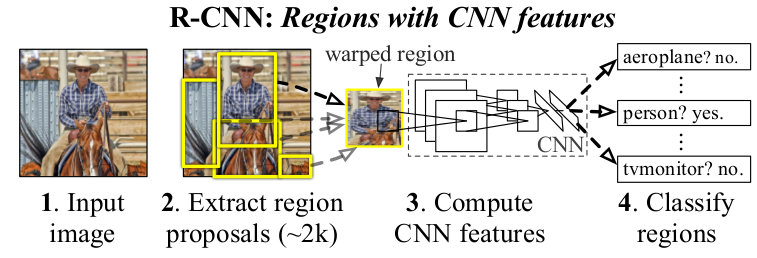
\includegraphics[width = \textwidth]{figures/RCNN/RCNN_overview.png}
\caption[Αρχιτεκτονική RCNN]{Πανόραμα του συστήματος εντοπισμού αντικειμένων του R-CNN \cite{10}. Το σύστημα λαμβάνει μια εικόνα (1), εξάγει 2000 προτεινόμενα περιβλήματα (2), υπολογίζει τα χαρακτηριστικά για κάθε ένα από τα περιβλήματα χρησιμοποιώντας ένα CNN (3), κατηγοριοποιεί κάθε περιοχή εντός κάποιου από τα προτεινόμενα περιβλήματα χρησιμοποιώντας linear SVM (4). Το R-CNN πετυχαίνει mAP ίσο με 53.7\% στο PASCAL VOC 2010 και 31.4 στο \textit{ILSVRC2013}.}
\label{fig:RCNN_overview}
\end{figure}

\section{Fast R-CNN \cite{11}}

Οι λόγοι για τους οποίους είναι αργό το R-CNN είναι δύο.
\begin{enumerate}
    \item Η χρήση του εμπρόσθιου περάσματος του AlexNet για κάθε πιθανού ορθογώνιου περιβλήματος από την Selective search το οποίο απαιτεί να εκτελεστεί το εμπρόσθιο πέρασμα του AlexNet περίπου 2000 φορές.
    \item Εκπαιδεύει τρία μοντέλα ξεχωριστά: το CNN για την εύρεση των χαρακτηριστικών της εικόνας, το SVM και το μοντέλο της απλής παλινδρόμισης για την βελτίωση των ορθογωνίων περιβλημάτων στο τέλος.
\end{enumerate}

Το Fast R-CNN υλοποιήθηκε με σκοπό να λύσει αυτά τα 2 προβλήματα και τελικά να επιταχύνει το R-CNN. Το πρώτο λύθηκε εκτελώντας τα βήματα σε διαφορετική σειρά. Πρώτα εκτελείται το εμπρόσθιο πέρασμα του CNN σε όλη την εικόνα και μετά γίνεται pooling σε κάθε πιθανό περίβλημα αντικειμένου (αυτό καλείται Region of Interest Pooling -RoIPool). Οπότε από περίπου 2000 εκτελέσεις του εμπρόσθιου περάσματος, πλέον απαιτείται μόνο μία. Το δεύτερο λύθηκε βάζοντας και τα τρία μοντέλα να εκτελούνται μαζί σε ένα κοινό δίκτυο. Η παλινδρόμηση γίνεται παράλληλα με την κατηγοριοποίηση η οποία πλέον δε γίνεται με SVM αλλά με \textit{Softmax classifier} λαμβάνοντας ως είσοδο το αποτέλεσμα του επίπεδου RoIPool. 

Η εκπαίδευση του δικτύου γίνεται 2.7 φορές πιο γρήγορα και οι χρόνοι αναγνώρισης αντικειμένων σε εικόνα ξεκινούν από 0.10 sec, ανάλογα με το μέγεθος της εικόνας. Η ακρίβεια (κριτήριο mAP) ελαφρώς αυξάνεται παρά τις αλλαγές στο δίκτυο.
Παρόλα αυτά οι χρόνοι εκτέλεσης συνεχίζουν να είναι απαγορευτικοί για ενσωματωμένα συστήματα. Επίσης δε γίνεται λόγος για κατανάλωση ενέργειας, διότι εκτελείται σε GPU (\textit{Nvidia K40 GPU overclocked to 875 MHz}). Επίσης αποφεύγεται η χρήση μεγάλων εικόνων, ώστε να μπορεί το δίκτυο να εμπεριέχεται ολόκληρο σε μια GPU και να μην απαιτείται πλέον χρήση του σκληρού δίσκου για caching. 

\begin{figure}
\centering
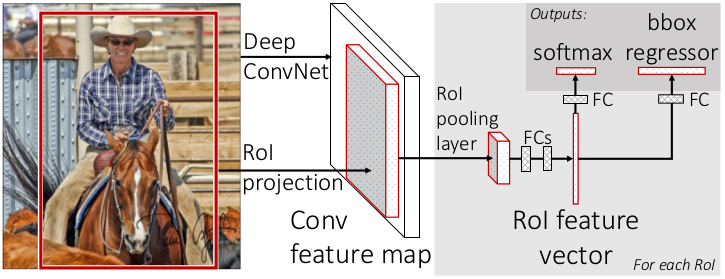
\includegraphics[width = \textwidth]{figures/RCNN/Fast-RCNN_architecture.png}
\caption[Αρχιτεκτονική Fast-RCNN]{Η αρχιτεκτονική Fast-RCNN \cite{11}. Η εικόνα εισόδου και οι πολλαπλές περιοχές ενδιαφέροντος (RoI) οι οποίες είναι είσοδοι σε ένα ενοποιημένο CNN. Κάθε RoI συλλέγεται σε ένα χάρτη χαρακτηριστικών δεδομένου μεγέθους και αντιστοιχίζεται σε ένα διάνυσμα χαρακτηριστικών χρησιμοποιώντας ολικά συνδεδεμένα επίπεδα (FCs στο Σχήμα \ref{fig:Fast_RCNN_architecture}). Το δίκτυο έχει δύο διανύσματα χαρακτηριστικών σε κάθε RoI. Ένα που προέρχεται από την έξοδο του Softmax και ένα από την γραμμική παλινδρόμηση. Τέλος το κομμάτι του ενοποιημένου δικτύου χρησιμοποιεί κοινή συνάρτηση απωλειών και όλα τα κομμάτια του εκπαιδεύονται μαζί.}
\label{fig:Fast_RCNN_architecture}
\end{figure}


\section{Faster R-CNN \cite{12}}
Η επόμενη -χρονικά- πρόταση ήταν το Faster R-CNN το οποίο προτάθηκε από το ερευνητικό τμήμα της \textit{Microsoft}. Το καινούριο αυτό δίκτυο βασίστηκε στο γεγονός ότι ο κύριος φόρτος εργασίας του Fast R-CNN γινόταν πλέον στον αλγόριθμο \textit{Selective Search}. Ταυτόχρονα, το βασικό δίκτυο επανα-υπολόγιζε χαρακτηριστικά (features) στις εικόνες στο πρώτο layer, τα οποία υπολόγιζε και η \textit{Selective Search} για να βρει τα περιβλήματα των αντικειμένων.

Επομένως η πρόταση για το Faster R-CNN ήταν η χρήση ενός νευρωνικού δικτύου RPN (\textit{Region Proposal Network}) το οποίο θα κάνει τη δουλειά της \textit{Selective Search}. Αυτό αποτελείται από δύο κομμάτια: ένα ολικά συνδεδεμένο επίπεδο που προτείνει περιοχές και τον ανιχνευτή του Fast R-CNN που χρησιμοποιεί τις προτεινόμενες περιοχές του πρώτου. Με αυτό τον τρόπο όλο το αρχικό R-CNN είναι πλέον ένα ενοποιημένο δίκτυο. Επιπλέον κατά τον εντοπισμό περιοχών αντικειμένων το RPN χρησιμοποιεί τη τεχνική της 'προσοχής'\cite{14} η οποία χρησιμοποιείται πλέον σε αρκετά νευρωνικά δίκτυα πέραν των συνελεκτικών για αύξηση της ακρίβειας.

\begin{figure}
\centering
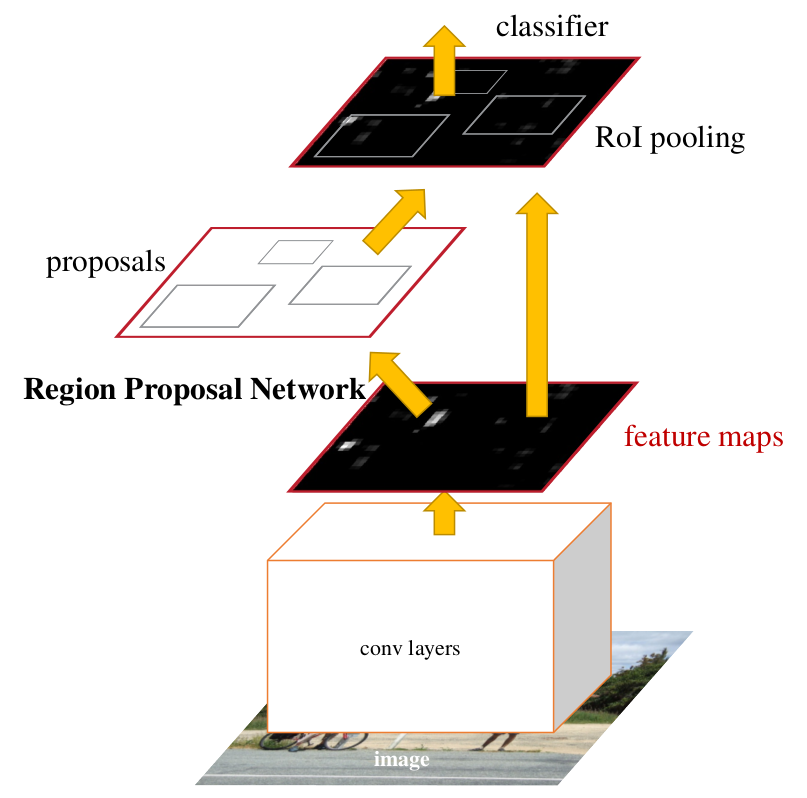
\includegraphics[width = \textwidth]{figures/RCNN/Faster-RCNN_RPN.png}
\caption[Η οντότητα RPN]{Η οντότητα RPN \cite{12}. Το δίκτυο Faster-RCNN είναι πλέον το ολοκληρωτικά ενοποιημένο δίκτυο για εντοπισμό αντικειμένων που εξελίχθηκε από το R-CNN. Η οντότητα RPN (\textit{Region Proposal Network}) βοηθά ως μέθοδος-τεχνική προσοχής αυτού του ενοποιημένου δικτύου, αντικαθιστώντας τη \textit{Selective Search}.}
\label{fig:Faster-RCNN_RPN}
\end{figure}

Αξιοσημείωτο είναι ότι το RPN χρησιμοποιείται από το SqueezeDet, αλλά αντί ολικά συνδεδεμένου δικτύου στο πρώτο χρησιμοποιεί συνελεκτικό επίπεδο. Και στις δύο περιπτώσεις υπάρχει ανεξαρτησία στη μετακίνηση των αντικειμένων.

Ουσιαστικά αυτό που συμβαίνει είναι ότι πάνω από τα αποτελέσματα του πρώτου επιπέδου τύπου CNN περνάει ένα παράθυρο το οποίο διαλέγει για κάθε εικονοστοιχείο της εικόνας $k$ πιθανά παράθυρα διαφορετικού μήκους και πλάτους. Οι χρόνοι εκτέλεσης είναι από 5 fps εώς 17 fps ανάλογα με τον τρόπο υλοποίησης του RPN σε GPU NVIDIA Tesla K40. Επίσης στο σύνολο δεδομένων \textit{PASCAL VOC 2012} πετυχαίνει ακρίβεια με κριτήριο mAP 59.9\%. H μνήμη ωστόσο συνεχίζει να αποτελεί πρόβλημα. Για αυτό δεν κρίνεται κατάλληλο για ενσωματωμένα συστήματα.

\section{Mask R-CNN \cite{13}}
Η τελευταία πρόταση βασισμένη στο R-CNN είναι το Mask R-CNN το οποίο προτάθηκε από την ερευνητική ομάδα της \textit{Facebook}. Το νευρωνικό δίκτυο αυτό είναι το Faster R-CNN με τη διαφορά πως αντί για ορθογώνια περιβλήματα των αντικειμένων πλέον εντοπίζει τα πραγματικά περιβλήματα στην εικόνα. Δηλαδή το σύνορο ενός αντικειμένου με την υπόλοιπη εικόνα δεν είναι πλέον ένα ορθογώνιο, αλλά ένα αφηρημένο σχήμα που το περιβάλλει με ακρίβεια εικονοστοιχείων. Για να επιτευχθεί αυτό χρησιμοποιείται ένας παράλληλος κλάδος του δικτύου, ο οποίος είναι υπεύθυνος για την κατηγοριοποίηση των εικονοστοιχείων σε αντικείμενα. Στο τέλος αυτού του κλάδου επιστρέφονται πίνακες οι οποίοι έχουν 1 στα εικονοστοιχεία στα οποία εντοπίζεται αντικείμενο και 0 σε αυτά που δεν εντοπίζεται. Κάθε πίνακας συνδέεται με ένα αντικείμενο σε ένα RoI. Αυτοί οι πίνακες είναι και οι μάσκες από όπου πήρε και το δίκτυο το ονομά του. Τέλος πρέπει να τονιστεί πως κάθε μάσκα βρίσκεται με παλινδρόμηση δύο κλάσεων αντικειμένων (δυαδική παλινδρόμηση) και όχι χρησιμοποιώντας \textit{Softmax}.

Προκειμένου να κατηγοριοποιηθεί ένα εικονοστοιχείο σε κάποιο αντικείμενο χρειάζεται να χρησιμοποιηθούν τα χαρακτηριστικά της εικόνας τα οποία υπολογίζονται χρησιμοποιώντας τα πρώτα συνελεκτικά επίπεδα του Faster R-CNN. Το πρόβλημα είναι πως οι διαστάσεις του τανυστή της εικόνας δεν είναι ίδιες με της διαστάσεις του τανυστή των χαρακτηριστικών. Έτσι αν μια περιοχή σημείων ήταν πάνω αριστερά και είχε διαστάσεις $15 \times 15$ πλέον θα έχει διαστάσεις $2.93 \times 2.93$ για χάρτη χαρακτηριστικών και εικόνα όπως παρουσιάζεται στο Σχήμα \ref{fig:Mask_RCNN_RoIAlign}. Σε αυτό το σημείο προτιμήθηκε να χρησιμοποιηθεί μια διγραμμική παρεμβολή, ώστε να υπολογίζονται τα χαρακτηριστικά των διαστάσεων με δεκαδικά. Αυτή η τεχνική λέγεται RoIAlign. Πρότερα, το εικονοστοιχείο που αντιστοιχούσε στη θέση $ x = 2.93$ των χαρακτηριστικών απλά θα αντιστοιχιζόταν στη θέση $ x = 2$.

\begin{figure}
\centering
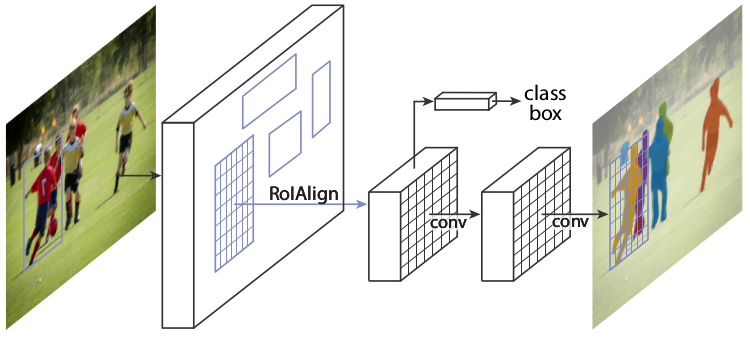
\includegraphics[width = \textwidth]{figures/RCNN/Mask-RCNN_RoIAlign.png}
\caption[RoIAlign]{Αντί του RoIPool, η εικόνα περνάει από το καινούριο επίπεδο RoIAlign \cite{13} ώστε οι περιοχές του χάρτη χαρακτηριστικών που διαλέγονται από το RoIPool να αντιστοιχούν με μεγαλύτερη ακρίβεια σε περιοχές της εικόνας εισόδου. Αυτό απαιτείται γιατί η κατηγοριοποίηση ανά εικονοστοιχείο  απαιτεί πιο λεπτομερή ευθυγράμμιση μεταξύ περιοχών της αρχικής εικόνας και του χάρτη χαρακτηριστικών.}
\label{fig:Mask_RCNN_RoIAlign}
\end{figure}

\begin{figure}
\centering
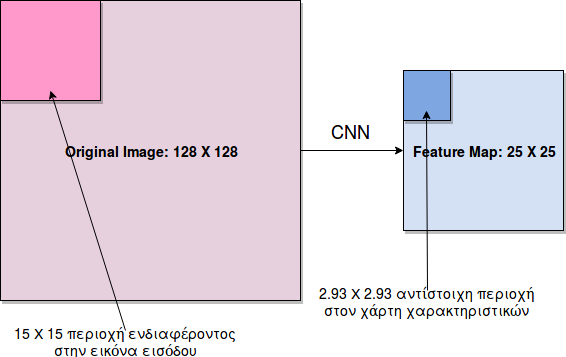
\includegraphics[width = \textwidth]{figures/RCNN/Mask-RCNN_RoIAlignExample.png}
\caption[Παράδειγμα RoIAlign]{Παράδειγμα αντιστοίχησης περιοχής από τον χάρτη χαρακτηριστικών στην αρχική εικόνα εισόδου. Για τον υπολογισμό των χαρακτηριστικών στο σημείο $(2.93, 2.93)$ χρησιμοποιείται διγραμμική παρεμβολή.}
\label{fig:Mask_RCNN_RoIAlignExample}
\end{figure}



Αυτή η κατηγοριοποίηση δίνει τη δυνατότητα για μεγαλύτερη ακρίβεια στον εντοπισμό αντικειμένων και φέρνει την αναγνώριση αντικειμένων πιο κοντά στα ανθρώπινα αποτελέσματα. Επιπλέον ο αλγόριθμος μπορεί να διαγωνιστεί και σε διαφορετικά περιβάλλοντα όπως το COCO όπου απαιτείται η κατηγοριοποίηση των εικονοστοιχείων από εικόνες σε αντικείμενα. Σε αυτό το σύνολο δεδομένων (COCO 2015, COCO 2016), η μέση ακρίβεια που επιτυγχάνει ο αλγόριθμος είναι $ mAP = AP = 37.1$, $ AP_{50} = 60.0 $, $AP_{75} = 39.4$, $ AP_S = 16.9$, $ AP_M = 39.9$, $ AP_L = 53.5 $ (μετρικές COCO \cite{15}). Η ταχύτητα εντοπισμού ανά εικόνα μένει ίδια στα 5 fps για το ίδιο hardware, διότι η καινούρια προσθήκη είναι ένα μικρό κομμάτι νευρωνικού δικτύου. Ταυτόχρονα, η μνήμη που χρειάζεται είναι περίπου η ίδια διότι το δίκτυο για τη μάσκα απαιτεί 355 kB το πολύ για Faster R-CNN τύπου FPN (Σχήμα \ref{fig:Mask_RCNN_architecture}).

\begin{figure}
\centerline{
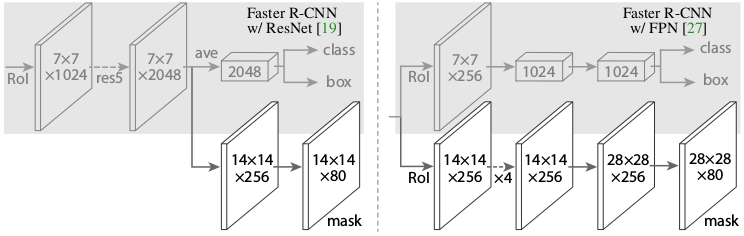
\includegraphics[width = \textwidth]{figures/RCNN/Mask-RCNN_architecture.png}
}
\caption[Αρχιτεκτονική Mask R-CNN]{Η αρχιτεκτονική Mask R-CNN \cite{13}. Η κεφαλή του δικτύου: Για την κεφαλή του δικτύου χρησιμοποιούνται κομμάτια από άλλα δίκτυα όπως το ResNet\cite{21} και το FPN\cite{22}. Τα βελάκια αντιστοιχούν σε συνέλιξη, αποσυνέλιξη ή πέρασμα από ένα ολικά συνδεδεμένο επίπεδο. Όλες οι συνελίξεις γίνονται από $3\times3$ φίλτρα, εκτός από τη συνέλιξη εξόδου, η οποία είναι $1\times1$. Οι αποσυνελίξεις γίνονται από $2\times2$ φίλτρα με βήμα 2. Επίσης η ενεργοποίηση χρησιμοποιεί ReLU στα κρυφά επίπεδα. Αριστερά φαίνεται η μάσκα του Mask-RCNN χρησιμοποιώντας το πέμπτο στάδιο του ResNet (res5) αλλαγμένο για περιοχή $7\times7$ με βήμα 1, αντί για $14\times14$ με βήμα 2. Δεξιά φαίνεται μια υλοποίηση της μάσκας του Mask-RCNN με τέσσερις διαδοχικές συνελίξεις πάνω στο Faster R-CNN με την κεφαλή του FPN.}
\label{fig:Mask_RCNN_architecture}
\end{figure}

Η εκπαίδευση γίνεται με τον ίδιο τρόπο όπως στο Fast R-CNN, χρησιμοποιώντας gradient descent με ορμή. Ωστόσο, τα RPN και το δίκτυο της μάσκας εκπαιδεύονται ξεχωριστά, θεωρώντας το RoI θετικό όταν η μετρική IoU είναι πάνω από 0.5. Επιπλέον τελικά χαρακτηριστικά που διερευνήθηκαν για το δίκτυο αυτό είναι:
\begin{itemize}
  \item Πολυκατηγορικές μάσκες ενάντια σε ανεξάρτητες μάσκες. Το αποτέλεσμα είναι ότι προτιμώνται οι ανεξάρτητες μάσκες οι οποίες μπορούν να υπολογιστούν μετά το RPN.
  \item Μάσκες ανά κατηγορία ή ανεξάρτητες. Το αποτέλεσμα είναι ότι οι ανεξάρτητες μάσκες έχουν πολύ μικρή διαφορά σε κριτήριο mAP από ότι αυτές που βρίσκονται ανά κατηγορία. Αυτό σημαίνει πως η πρόβλεψη μια μάσκας $ m \times m $ είναι πιο συμφέρουσα από ότι να έχω μία μάσκα για κάθε πιθανή κλάση του εντοπισμένου αντικειμένου.
\end{itemize}

Βέβαια λόγω των υπολογιστικών απαιτήσεων το δίκτυο αυτό δε θεωρείται κατάλληλο για ενσωματωμένα συστήματα. Παρ' όλα αυτά η δυνατότητα εντοπισμού αντικειμένων ανά εικονοστοιχείο το χρήζει πιο εύχρηστο για άλλους αλγορίθμους που χρησιμοποιούνται σε αυτά, όπως το SLAM με vision, η αυτόνομη οδήγηση κ.α. 



% \section{Inception-v4 \cite{17}}
% να δώσω έμφαση στο Inception module και στο πως μπορεί να γίνει retrain


% \section{ResNet}

\section{XNOR-Net \cite{18}}

Το δίκτυο XNOR προσεγγίζει διαφορετικά το πρόβλημα των CNN από ότι όλα τα παραπάνω. Η διαφορά έγκειται στη χρήση δυαδικών βαρών και αναπαράσταση της εισόδου ως δυαδικής. Η προσέγγιση αυτή καθιστά δυνατή την εκτέλεση του δικτύου όχι μόνο σε GPU ή εξειδικευμένο hardware όπως \textit{FPGA} ή \textit{ASIC}, αλλά και σε CPU. Περαιτέρω στην πρόταση του νευρωνικού εξετάζονται δύο εκδοχές
\begin{enumerate}
  \item Μόνο δυαδικά βάρη που δέχονται τιμές στο σύνολο $\{-1, +1\}$.
  \item Ταυτόχρονα δυαδικά βάρη και δυαδική είσοδος που δέχονται τιμές στο σύνολο $\{-1, +1\}$.
\end{enumerate}
Η δεύτερη από τις δύο εκδοχές είναι και η πιο αποτελεσματική, τόσο από άποψη χρόνου εκτέλεσης, όσο και από άποψη ακρίβειας. Και στις δύο περιπτώσεις η αρχιτεκτονική του δικτύου είναι ίδια με κάποιο άλλο π.χ. AlexNet\cite{20}, GoogleNet\cite{17}, ResNet\cite{21}. Αυτό που αλλάζει είναι τα βάρη και η σειρά με την οποία γίνονται οι πράξεις. Δηλαδή σε ένα κοινό δίκτυο έχουμε πρώτα τη συνέλιξη($C$), μετά την κανονικοποίηση($B$), αργότερα την ενεργοποίηση($A$) και τέλος τη συγκέντρωση ($P$). Στο δίκτυο XNOR η σειρά είναι διαφορετική: $B\rightarrow A\rightarrow C\rightarrow P$.

\begin{figure}
\centering
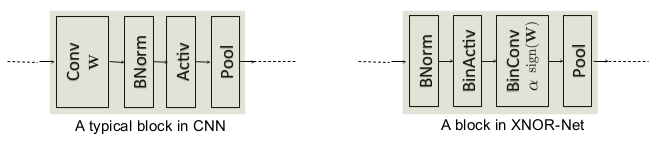
\includegraphics[width = \textwidth]{figures/XNOR_Net/XNOR_NET_block.png}
\caption[XNOR block vs typical CNN block]{Σύγκριση μεταξύ των μπλοκ του XNOR-Network (δεξιά) και ενός τυπικού CNN (αριστερά) \cite{18}.}
\label{fig:XNOR_NET_block}
\end{figure}

Για να είναι επιτυχής η προσαρμογή του δικτύου σε διάφορες αρχιτεκτονικές οι συγγραφείς επινόησαν έναν αλγόριθμο για το μετασχηματισμό της εισόδου και των βαρών στο σύνολο των δυαδικών τανυστών. Σε αυτό το σύνολο τανυστών τα στοιχεία κάθε τανυστή λαμβάνουν τιμές στο σύνολο $\{-1, +1\}$. Πιο αναλυτικά: Έστω η κανονική είσοδος ενός επιπέδου $I$ και έστω $W$ το σύνολο των βαρών αυτού του επιπέδου. Τότε σύμφωνα με τον προτεινόμενο αλγόριθμο:
    $$ \mathbf{I} \ast \mathbf{W} \approx (sign(\mathbf{I}) \circledast sign(\mathbf{W}) ) \odot \mathbf{K} \alpha  $$

Ο τελεστής $ \circledast$ αντιπροσωπεύει συνέλιξη με χρήση XNOR αντί για πολλαπλασιασμού.
Οπότε ο μετασχηματισμένος πίνακας εισόδου είναι ο $ sign(\mathbf{I}) $ και ο μετασχηματισμένος πίνακας βαρών είναι ο $ sign(\mathbf{W}) $.
Ο τελευταίος όρος είναι ένας πίνακας που πολλαπλασιάζεται στοιχείο ανά στοιχείο για να κλιμακωθεί σωστά το αποτέλεσμα της συνέλιξης ($  \circledast $) με XNOR.

\begin{figure}
\centering
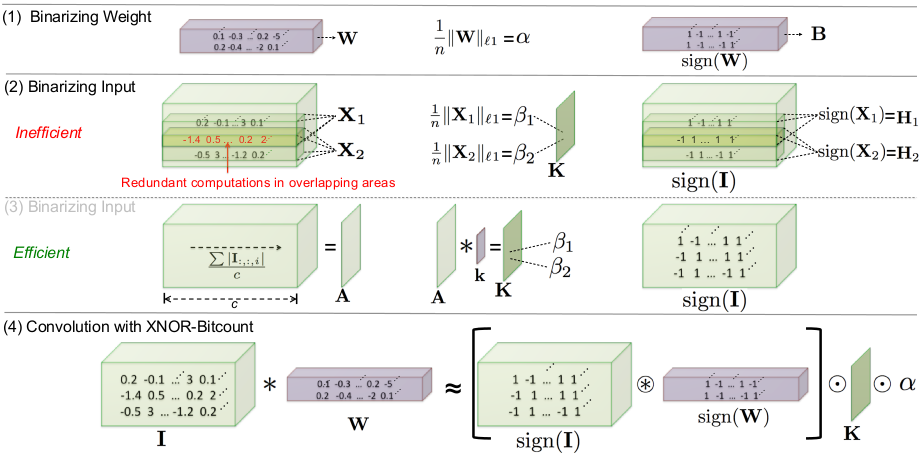
\includegraphics[width = \textwidth]{figures/XNOR_Net/XNOR_NET_procedure.png}
\caption[Αποτύπωση της συνέλιξης στο XNOR Net]{Επεξήγηση της διαδικασίας μετασχηματισμού της συνέλιξης σε συνέλιξη που κάνει χρήση της πράξης XNOR και δυαδικούς τανυστές \cite{18}.}
\label{fig:XNOR_NET_procedure}
\end{figure}

Όσον αφορά την εκπαίδευση το δίκτυο χρησιμοποιεί τη τεχνική ADAM \cite{19} και πετυχαίνει καλύτερη ακρίβεια από ότι αν χρησιμοποιούσε στοχαστική \textit{gradient descent} (\textit{SGD}). Επίσης είναι το πρώτο δυαδικό δίκτυο που έχει ελεγχθεί στο διαγωνισμό του \textit{ImageNet}. Στην ακρίβεια μεταξύ των κορυφαίων 5 κλάσεων χρησιμοποιώντας την αρχιτεκτονική του \textit{AlexNet} πετυχαίνει σκορ 69.2 και της κορυφαίας μίας 44.2. Αντίστοιχα χρησιμοποιώντας την αρχιτεκτονική του \textit{ResNet} πετυχαίνει 73.2 και 51.2. Αν χρησιμοποιούσε κανείς το \textit{ResNet} από μόνο του θα πετύχαινε ακρίβεια 89.2 για τις κορυφαίες 5 και 69.3 για τη κορυφαία μία. Βέβαια αυτή η θυσία της ακρίβειας γίνεται προς αύξηση της ταχύτητας, η οποία είναι ~$32\times$ φορές πιο αυξημένη. Μεγαλύτερη επιτάχυνση δικτύων επιτυγχάνεται όσο τα φίλτρα στα επίπεδα του νευρωνικού είναι μεγαλύτερα. Αυτό βέβαια βρίσκεται σε αντίθεση με τη πιο μοντέρνα τακτική να ελαττώνονται οι διαστάσεις των δικτύων όπως στο \cite{23}. 
Από πλευράς ενεργειακής αποδοτικότητας δε γίνεται λόγος στη σχετική έρευνα. Παρόλα αυτά, από τη στιγμή που το δίκτυο απαιτεί λιγότερες πράξεις από πολλαπλασιασμούς και είναι μικρότερο σε μέγεθος εξοικονομείται τόσο ενέργεια από τον επεξεργαστή όσο και από τη χρήση της DRAM.


\section{SSD \cite{26}}
Το δίκτυο αυτό παρουσιάζει κοινή αρχιτεκτονική με το Faster-RCNN και ουσιαστικά αποτελεί μια βελτίωση του (Deep Multibox \cite{27}). Η διαφορά του από άλλα δίκτυα είναι ότι διακριτοποιεί τις προβλέψεις για τα ορθογώνια περιβλήματα αντικειμένων σε ένα σύνολο από προκαθορισμένα aspect ratios και μεγέθη ανά περιοχή του (feature map). Κατά τον χρόνο εκτέλεσης το νευρωνικό εξάγει σκορ για την παρουσία κάθε κλάσης αντικειμένων σε κάθε ένα από τα προκαθορισμένα περιβλήματα και παράγει διορθώσεις ώστε κάθε περίβλημα να ταιριάξει στο μέγεθος του αντικειμένου. Επιπλέον το δίκτυο συνδυάζει προβλέψεις από πολλαπλά (feature maps) με διαφορετικές αναλύσεις για τη φυσική αντιμετώπιση αντικειμένων διαφόρων μεγεθών.

Το SSD είναι πιο απλό σε σχέση με τις μεθόδους που απαιτούν την ύπαρξη δικτύου για να προτείνει αντικείμενα, γιατί καταργεί εντελώς τα ξεχωριστά επίπεδα που παράγουν προτάσεις αντικειμένων και αυτά που τα ακολουθούν για αναδειγματοληψία ανά εικονοστοιχείο (ή ανά feature) και τοποθετεί όλους τους υπολογισμούς σε ένα δίκτυο. Αυτό καθιστά το δίκτυο εύκολο στην εκπαίδευση και στην ενσωμάτωση του σε άλλα συστήματα.

Οι πειραματισμοί στα σύνολα δεδομένων PASCAL VOC, COCO και ILSVRC επιβεβαιώνουν ότι το SSD έχει ανταγωνιστική ακρίβεια σε σχέση με άλλες μεθόδους που χρησιμοποιούν επιπλέον βήματα για την πρόταση του αντικειμένου. Ταυτόχρονα, είναι πιο γρήγορο και προσφέρει μια ενοποιημένη δομή τόσο για την εκπαίδευση όσο και για την απλή εκτέλεση. Για εικόνες εισόδου $ 300 \times 300 $ (SSD300) το δίκτυο επιτυγχάνει mAP 74.3\% στο σύνολο δεδομένων VOC2007 στα 59 FPS χρησιμοποιώντας την GPU Nvidia Titan X. Ενώ για εικόνες εισόδου $ 512 \times 512 $ επιτυγχάνει mAP 76.9\% υπερβαίνοντας την απόδοση του Faster-RCNN. 

Συγκρινόμενο με άλλες μεθόδους με ένα στάδιο, το SSD έχει κατά πολύ καλύτερη ακρίβεια ακόμα και με μικρότερη εικόνα εισόδου. Αυτό το χρήζει ικανό για να χρησιμοποιηθεί σε ενσωματωμένα συστήματα, αφού οι απαιτήσεις μνήμης του είναι μικρότερες, λόγω του μονού σταδίου και είναι αρκετά γρήγορο για την εκτέλεσή του. 

\section{Σύνοψη}
Στα προηγούμενα μέρη του κεφαλαίου αναλύσαμε κάθε δίκτυο ξεχωριστά παρουσιάζοντας την αρχιτεκτονική, την ακρίβειά και την ταχύτητά του. Επίσης, συμπεράναμε κατά πόσο το κάθε ένα μπορεί να χρησιμοποιηθεί σε ενσωματωμένη συσκευή. Από εκεί προέκυψε πως τα δίκτυα τα οποία μπορούν να χρησιμοποιηθούν για εντοπισμό αντικειμένων είναι τα:
\begin{itemize}
    \item SqueezeDet
    \item YOLO
    \item YOLO9000
    \item SSD
\end{itemize}

\subsection*{Από άποψη χρόνου εκτέλεσης}

Στη βιβλιογραφία διακρίνονται δύο είδη δικτύων: για εντοπισμό αντικειμένου (object localization) και για αναγνώριση αντικειμένου (object recognition). Τα πρώτα μελετούνται ως προς το χρόνο εκτέλεσης και την ακρίβεια (mAP). Τα δεύτερα ως προς τον αριθμό παραμέτρων, τον χρόνο εκτέλεσης, την ακρίβειά τους και το πόσο καλά μπορούν να εκπαιδευτούν. Επίσης, τα δίκτυα εντοπισμού εμπεριέχουν μέσα δίκτυα για εξαγωγή χαρακτηριστικών(feature extraction). Οπότε παρατίθενται οι δύο πίνακες για δίκτυα που κάνουν feature extraction (Πίνακας \ref{table:cnnComp}) και για δίκτυα που κάνουν εντοπισμό αντικειμένων (Πίνακας \ref{table:detCnnComp}).

Τα δίκτυα YOLO και SSD αν και προτείνονται για ενσωματωμένα, στα πειράματα που έχουν γίνει απαιτούν αρκετούς πόρους ακόμα και για ενσωματωμένες συσκευές, διότι εκτελούνται μόνο σε GPU. Επειδή γενικότερα στην βιβλιογραφία επικρατεί μία σύγχυση για τους χρόνους εκτέλεσης των νευρωνικών δικτύων στο παρόν κείμενο χρησιμοποιήθηκε η μετρική frame/ms/Watt , όπου μετριέται ο χρόνος εκτέλεσης ως προς την κατανάλωση ισχύος στο 'forward pass' του νευρωνικού ανά frame. Κατά αυτό τον τρόπο υπάρχει ένα μέτρο το οποίο μπορεί να συγκρίνει τους χρόνους εκτέλεσης ανεξαρτήτως της αρχιτεκτονικής. Ωστόσο, υπάρχει το μειονέκτημα ότι διαφορετικές αρχιτεκτονικές χρησιμοποιούν διαφορετικά ποσά ενέργειας για να πραγματοποιήσουν τις ίδιες πράξεις.


Από άποψη ακρίβειας το επικρατέστερο δίκτυο (από αυτά που αναλύονται) είναι το Faster-RCNN. Παρόλα αυτά, τα δίκτυα δεν μπορούν να συγκριθούν με το Mask-RCNN γιατί αυτό δεν βρίσκει ορθογώνια περιβλήματα μόνο αλλά κάνει και εντοπισμό των αντικειμένων της εικόνας ανά εικονοστοιχείο. Για τα υπόλοιπα η σειρά ακρίβειας είναι η παρακάτω.
\begin{enumerate}
    \item Faster-RCNN
    \item SqueezeDet
    \item YOLO9000
    \item SSD
    % \item XNOR-Net
\end{enumerate}

Αξιοσημείωτο είναι ότι το SSD πετυχαίνει καλύτερη ακρίβεια, όση και το Faster-RCNN με χρόνους εκπαίδευσης διπλάσιους του YOLO. Επίσης ότι το SqueezeDet μπορεί και ξεπερνάει την ακρίβεια του Faster-RCNN σε κάποια σύνολα δεδομένων. Το τελευταίο στη λίστα είναι το δίκτυο XNOR-Net το οποίο έχει μεγάλη διαφορά από τα άλλα δίκτυα σε ακρίβεια. Όπως αναφέρεται και στη σχετική δημοσίευση \cite{18}, το XNOR-Net προσπαθεί να λύσει το πρόβλημα εκτέλεσης νευρωνικού σε CPU χρησιμοποιώντας bits για την αναπαράσταση των παραμέτρων του και όχι Bytes, προκειμένου να το χωρέσει στη διαθέσιμη μνήμη που διαθέτει μία συμβατική ενσωματωμένη συσκευή. Η χρησιμότητα του όμως αίρεται στη γενική περίπτωση, με τη λογική ότι το SqueezeDet μπορεί να πετύχει αρκετά μεγαλύτερη ακρίβεια έχοντας μικρότερο μέγεθος. Χρήσεις του XNOR-Net αφορούν περισσότερο σχεδιαστικά προγράμματα π.χ. για αναγνώριση αντικειμένων από σκίτσα \cite{33}.

\subsection*{Από άποψη μνήμης}
Τα δίκτυα για feature extraction μελετώνται πλέον με τον αριθμό των παραμέτρων. Αυτό γίνεται διότι η αναπαράστασή τους σε 8, 16 ή 32 bit καθορίζεται από τους επιπλέον αλγόριθμους συμπίεσης (π.χ. Ristretto \cite{28}). Ο Πίνακας \ref{table:cnnComp} δείχνει τα χαρακτηριστικά κάθε νευρωνικού τέτοιου τύπου. Οι χρόνοι αφορούν την εκτέλεση των δικτύων αυτών με τη χρήση του tensorflow \cite{34} στη GPU GTX 1080 Ti της NVIDIA, και στο σύνολο δεδομένων του Imagenet ILSVRC2012. Οι υπολογισμοί τους έγιναν για το σκοπό αυτής της διπλωματικής στη συστοιχία του εργαστηρίου Αρχιτεκτονικής και συστημάτων που αναλύεται σε παρακάτω κεφάλαιο. Παρά ταύτα, παρατίθενται και οι χρόνοι για δίκτυα που δεν ενδείκνυται η εκτέλεσή τους σε GPU, σε άλλη πλατφόρμα.


\begin{table}
\centering
% \captionof{table}{YOLOv2 features} \label{tab:title}
\begin{tabular}{c|c|c|c} 
 Δίκτυο feature extraction & Top-1 ακρίβεια & Αριθμός Παραμέτρων & frames/ s /W \\
\hline
% SqueezeNet & 57.5 & 421,098 (6 bit) & $68.4\, ms / 2W$ \\ % NAO ATOM
SqueezeNet & 57.5 & 421,098 (6 bit) & $ 9.429 $ \\ % GTX 1080 Ti
XNOR-Net & 44.2 & 61M (61MB) & $439.56 \text{fps}\, / 2W$ (ATOM Z530 CPU) \\ % 
VGG-16 & 70.5 & 14,714,688 & $2.225$ \\ %GTX 1080 Ti
MobileNet-224 & 83.3 & 3,191,072 & $45.278$ \\ %
ResNet-101 V2& 76.4 & 42,605,504 & $2.316$ \\ %GTX 1080 Ti
% Inception V2 & 73.9 & 10,173,112 & \\
Inception V3 & 78.0 & 21,802,784 & $ 2.4276$ \\  %GTX 1080 Ti
Inception V4 & 80.4 & 54,336,736 & $ 1.3816$ \\ %GTX 1080 Ti, Inception V4
\hline
\end{tabular}
\caption[Σύγκριση δικτύων για feature extraction]{Σύγκριση δικτύων για feature extraction στο εμπρόσθιο πέρασμα για ένα frame. Όλα τα δίκτυα έχουν παραμέτρους σε αναπαράσταση float32 εκτός από το XNOR-Net και μόνο αυτό εκτελείται σε CPU. Η ακρίβεια των δικτύων μετριέται στο σύνολο δεδομένων του ImageNet. Τα χαρακτηριστικά των δικτύων που δεν αναλύονται στο κεφάλαιο είναι από \cite{28}, ενώ άλλα προέρχονται από \cite{29}, 
\cite{30, 31, 32}. Οι εικόνες για την μέτρηση είναι στο μέγεθος των εικόνων του ImageNet. Αν η πλατφόρμα εκτέλεσης του δικτύου είναι διαφορετική, τότε αυτή αναγράφεται μέσα σε παρενθέσεις. Οι παραπάνω υπολογισμοί έγιναν στη συστοιχία του εργαστηρίου, εκτός από αυτούς που δίνονται για το XNOR-Net οι οποίοι υπολογισμοί έγιναν σε επεξεργαστή \textit{ATOM Z530}.}
\label{table:cnnComp}
\end{table}

\begin{table}
\vspace{-5em}
% \centering
\begin{tabular}{c|c|c} 
 Δίκτυο Εντοπισμού & mAP & Χρόνος Εκτέλεσης / frame / W \\
\hline
SqueezeDet + SqueezeNet & 80.4 (KITTI)&$31.2\, ms / 128.3 W$ (NVIDIA Titan X)\\ % 
YOLO9000 $480\times480$ + Darknet & 77.8 (PASCAL VOC 7+12) & $ 17\, ms / 250 W$ (NVIDIA Titan X) \\ % 
% XNOR-Net & 44.2 () & $2.275 ms\, / 2W$ (NAO ATOM) \\ % 
SSD300 + VGG16 & 74.3 (PASCAL VOC 7+12) & $ 52\,ms / 250 W$ (NVIDIA Titan X) \\
Mask R-CNN + ResNeXt-101 & 37.1 (MS COCO 2015) & \~$240\,ms / 143.1 W$ (NVIDIA Titan X)\\
Faster R-CNN + ResNet & 76.4 (PASCAL VOC 7+12)& $200\,ms / 143.1 W$ (NVIDIA Titan X)\\
\hline
\end{tabular}
\caption[Σύγκριση δικτύων για εντοπισμό αντικειμένων]{Σύγκριση δικτύων για εντοπισμό αντικειμένων. Η ακρίβεια των δικτύων μετριέται σε διάφορα σύνολα δεδομένων. Η παράθεση αυτή γίνεται, διότι δεν υπάρχει κάποιο κοινό σύνολο δεδομένων στο οποίο να έχουν εκτελεσθεί όλα τα δίκτυα εντοπισμού, σε αντίθεση με τα απλά CNN. Βέβαια αυτό γίνεται για λόγους που αφορούν την ακρίβεια και θα εξετασθούν αναλυτικότερα στο επόμενο κεφάλαιο.}
\label{table:detCnnComp}
\end{table}

Το RCNN και οι απόγονοί του τοποθετήθηκαν κυρίως για να φανεί η σειρά στην οποία όλοι βασίστηκαν κατά την ανάπτυξη των νευρωνικών δικτύων εντοπισμού αντικειμένων. Όλες οι παραπάνω προτάσεις συγκρίνονται με τα Fast-RCNN και Faster-RCNN και όπως φαίνεται τα επόμενα θα συγκριθούν με το Mask-RCNN. Μάλιστα όπως το SqueezeDet εμπνεύστηκε από το Faster R-CNN έτσι και ένα επόμενο δίκτυο ενσωματωμένων μπορεί να εμπνευστεί από το Mask R-CNN. Ήδη παρόμοια λειτουργία σε ενσωματωμένα συστήματα πραγματοποιεί το ENet \cite{16}.
 % do corrections
\chapter{Μετάδοση Γνώσης}%
\label{chapter:tl}
\section{Εισαγωγή}
Ο όρος της μετάδοσης γνώσης(Transfer Learning) χρησιμοποιείται σε όλο το φάσμα της τεχνητής νοημοσύνης ως η μεταφορά παραμέτρων ενός ήδη εκπαιδευμένου συστήματος σε ένα άλλο. Στο παρόν κεφάλαιο θα αναλυθεί η μετάδοση γνώσης σε αλγορίθμους εντοπισμού αντικειμένων· βέβαια για την καλύτερη ανάλυση αρχικά θα πρέπει να δοθούν κάποιοι ορισμοί και να ερμηνευτεί με ακρίβεια ο όρος. Έπειτα, θα αναλυθούν οι τρόποι μετάδοσης γνώσης όπως φαίνονται στο Σχήμα \ref{fig:TL_categories}. Στο τέλος παρουσιάζεται το πείραμα αυτής της εργασίας για τα δίκτυα εντοπισμού αντικειμένων.

\begin{figure}
    \centering
    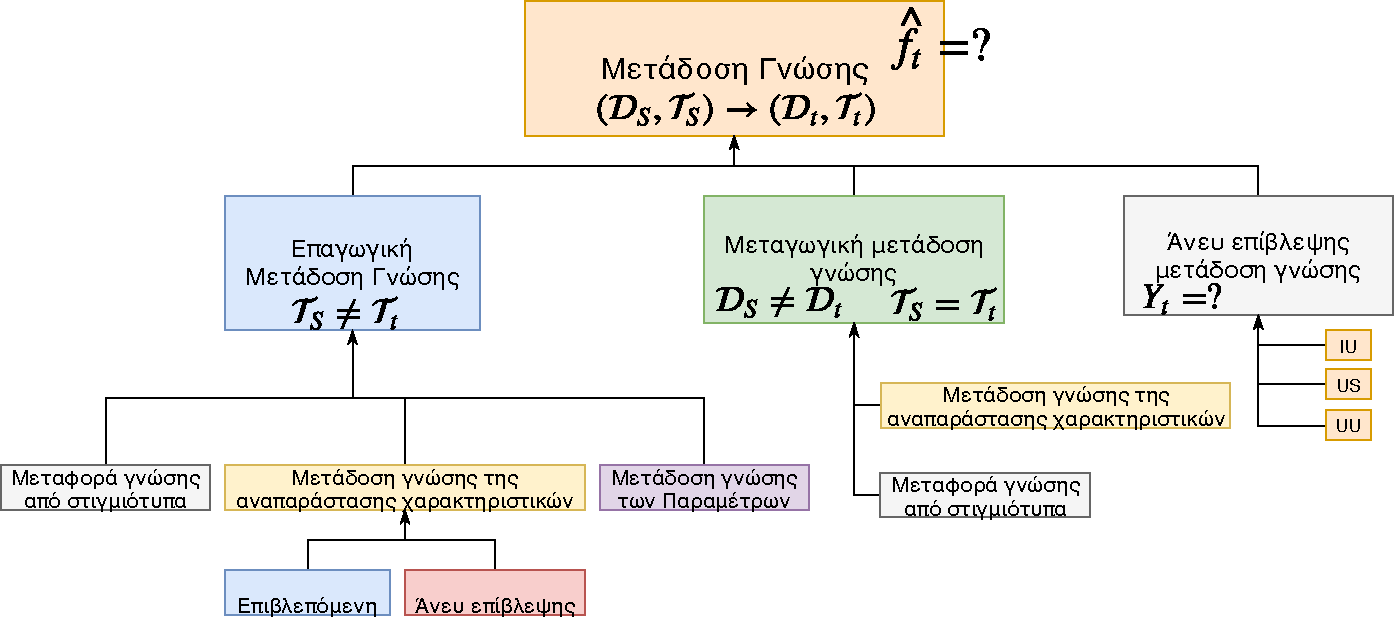
\includegraphics[width = 0.8\textwidth]{figures/transferLearning/TL_categorisation.pdf}
    \caption[Οι κατηγορίες της μετάδοσης γνώσης]{Η κατηγοριοποίηση των διάφορων ειδών μετάδοσης γνώσης. Στο πρώτο (πάνω) επίπεδο φαίνεται η φορά πληροφορίας και ο τελικός σκοπός όλης της μετάδοσης γνώσης. Στο δεύτερο επίπεδο φαίνεται οι σχέσεις μεταξύ του αρχικού και τελικού προβλήματος στα τρία σενάρια μετάδοση γνώσης. Στο τελευταίο επίπεδο παρουσιάζονται οι διάφορες προσεγγίσεις σε κάθε μία από τις κατηγορίες. Όλα αυτά αναλύονται με λεπτομέρεια στο παρόν κεφάλαιο.}
    \label{fig:TL_categories}
\end{figure}

\section{Πρόβλημα}
Το πρόβλημα που αντιμετωπίζεται στα νευρωνικά δίκτυα έγκειται στο θεώρημα \textit{no free lunch} \cite{37}. H
θεωρία της μηχανικής μάθησης υποστηρίζει ότι οι αλγόριθμοι μηχανικής μάθησης μπορούν να γενικευτούν σε ένα πεπερασμένο σύνολο από παραδείγματα. Ωστόσο, αυτό δείχνει να αντιτίθεται σε κάποιες βασικές αρχές της λογικής. Η επαγωγή γενικών κανόνων από κάποιο πεπερασμένο σύνολο παραδειγμάτων δεν αποτελεί λογικό εγχείρημα. Για παράδειγμα, προκειμένου να δημιουργηθεί ένας κανόνας ο οποίος να περιγράφει κάθε μέλος ενός συνόλου, θα πρέπει εκ των προτέρων να υπάρχει πληροφορία για κάθε μέλος αυτού του συνόλου.

Εν μέρει η μηχανική μάθηση προσπερνά αυτό το πρόβλημα προσφέροντας μόνο πιθανοτικούς κανόνες, αντί για ακριβείς κανόνες που αποτελούν μέλη της μαθηματικής λογικής. Η μηχανική μάθηση υπόσχεται να βρει κανόνες οι οποίοι είναι πιθανοτικά έγκυροι για τα περισσότερα μέλη κάποιου συνόλου. Δυστυχώς, ακόμη και αυτό δεν μπορεί να επιλύσει το όλο πρόβλημα. Σύμφωνα με το θεώρημα \textit{no free lunch}, ο μέσος όρος σφάλματος σε όλες τις πιθανές κατανομές σημείων εισόδου, για κάθε αλγόριθμο κατηγοριοποίησης είναι ο ίδιος με την κατηγοριοποίηση σημείων τα οποία δεν έχουν παρατηρηθεί εκ των προτέρων.

Αν $ \mathbb{K} $ είναι το σύνολο όλων των πιθανών κατανομών και $ \kappa_i, \kappa_j \in \mathbb{K}$ δύο κατανομές στις οποίες έχουν εκπαιδευτεί
οι αλγόριθμοι $a_i, a_j$ αντίστοιχα. Τότε για συνάρτηση σφάλματος $e(a,\kappa)$ αλγορίθμου $a$ σε κάποια κατανομή $\kappa \in \mathbb{K}$, ισχύει:
$$ \EX_{\kappa \in \mathbb{K}-\kappa_i}\left[ e(a_i, \kappa) \right] = \EX_{\kappa \in \mathbb{K}-\kappa_j}\left[ e(a_j, \kappa) \right], \forall i,j
$$ 

Δηλαδή, κανένας αλγόριθμος δεν είναι καλύτερος στην επίλυση καινούριων προβλημάτων από ότι ένας άλλος. Ευτυχώς,
αυτό συμβαίνει μόνο όταν λαμβάνονται υπόψη όλες οι πιθανές κατανομές. Στον πραγματικό κόσμο μπορούν να γίνουν κάποιες
υποθέσεις για τους τύπους κατανομών που αντιμετωπίζονται και μπορεί να γίνει ο ισχυρισμός ότι αυτές ανήκουν σε συγκεκριμένες πολλαπλότητες.
Παρόλα αυτά, απαιτείται το δίκτυο εντοπισμού να είναι πραγματικού χρόνου και περιορισμένης μνήμης. Έτσι, δεν μπορεί 
να συμπεριλάβει χαρακτηριστικά για να αφομοιώσει όλη την εμπειρία που απαιτείται για να εντοπίζει εκ των προτέρων κάθε αντικείμενο.

\section{Μία ιδέα για τη μετάδοση γνώσης \cite{38}}
Η μετάδοση γνώσης είναι μία ανθρώπινη διαδικασία η οποία έχει μελετηθεί πολύ στην
φιλοσοφία, στην εκπαίδευση και στην εκπαιδευτική ψυχολογία \cite{39}. Στην εκπαίδευση, η μετάδοση
γνώσης αναφέρεται ως:
"Προηγουμένως μαθημένες γνώσεις ή ικανότητες οι οποίες επηρεάζουν τον τρόπο με τον οποίο
μία καινούρια γνώση ή ικανότητα μαθαίνεται και χειρίζεται. Η μετάδοση θεωρείται ως θετική
αν η απόκτηση και η επίδοση στην χρήση της καινούριας γνώσης διευκολύνθηκε και ως αρνητική
αν εμποδίστηκε."(μετάφραση από: \cite{76})

Όταν η τεχνική μετάδοσης γνώσης εφαρμόζεται στη μηχανική μάθηση έχει παρόμοιο σκοπό. Το κίνητρο της μηχανικής μάθησης είναι να βελτιώσει τη μάθηση σε ένα συγκεκριμένο πεδίο αποκτώντας πληροφορία από ένα παρόμοιο, αλλά διαφορετικό πεδίο. Οι παραδοσιακές τεχνικές μηχανικής μάθησης, όπως λέχθηκε λειτουργούν υπό υποθέσεις για τις κατανομές τους. Για αυτό και παλαιότερα προτεινόταν η μάθηση να αρχίζει \textit{tabula rasa}, χωρίς να ξέρει τίποτε πιο πριν ο αλγόριθμος και όλοι οι παράμετροι των δικτύων ή των αλγορίθμων να αρχίζουν από κάποια τυχαία κατανομή όπως η γκαουσιανή. Επιπλέον, υπάρχει η ανάγκη από την πλειοψηφία των τεχνικών μηχανικής μάθησης τα δεδομένα στα σύνολα της εκπαίδευσης και του ελέγχου να είναι από τον ίδιο χώρο χαρακτηριστικών (feature space).
Η τεχνική μετάδοσης γνώσης δείχνει πως αυτό δεν είναι σε κάθε περίπτωση απαραίτητο για τα νευρωνικά δίκτυα, γιατί δίνεται η δυνατότητα να συνδυαστεί προηγούμενη γνώση από μία προηγούμενη εκπαίδευση σε μία καινούρια αλλά σχετική με την προηγούμενη.

Χρησιμοποιώντας αυτή την παρατήρηση μπορεί να παρακάμψει κανείς το \textit{no free lunch theorem}, 
διότι δεν χρειάζεται ανά πάσα στιγμή να είναι δυνατός ο εντοπισμός όλων των αντικειμένων. Ο αλγόριθμος μπορεί  να ξέρει κάθε στιγμή να εντοπίζει ένα μικρό σύνολο αντικειμένων και απλά κάθε φορά να μαθαίνει τον εντοπισμό ενός καινούριου συνόλου.

\section{Ορισμός της Μετάδοσης Γνώσης \cite{40, 41}}
Πριν τη μετάβαση στον μαθηματικό ορισμό της τεχνικής μετάδοσης γνώσης θα πρέπει να ορισθούν κάποια άλλα μεγέθη
πρώτα. Οι ορισμοί αυτοί μπορούν να χρησιμοποιηθούν γενικότερα στο αντικείμενο της μηχανικής μάθησης, ωστόσο συνίσταται η χρήση τους μόνο στο αντικείμενο της μετάδοσης γνώσης.
\vspace{1ex}\\
{ \rule{1ex}{1ex} }%
\textit{Το πεδίο ορισμού(\textit{Domain}) ορίζεται ως μία δυάδα $D = (\mathcal{X},P)$. Το πρώτο μέλος της δυάδας $\mathcal{X}$ είναι ο χώρος (πολλαπλότητα) στον οποίο ανήκουν τα δείγματα-παρατηρήσεις $x$ κάποιου προβλήματος (π.χ. ο χώρος των διδιάστατων εικόνων για εικόνες μεγέθους $1024 \times 768$). Το δεύτερο μέλος της δυάδας είναι η αθροιστική συνάρτηση κατανομής $P(X)$ όπου $X = {x_1 , \cdots , x_n } \in \mathcal{X}$. }

Η εκπαίδευση, η οποία ορίζεται και παρακάτω, γίνεται πάντα σε ένα πεπερασμένο κομμάτι του πεδίου ορισμού, διότι εκτελείται από κάποιον αλγόριθμο και διαρκεί πεπερασμένο χρόνο.
\vspace{1ex}\\
{ \rule{1ex}{1ex} }%
\textit{Δοθέντος ενός πεδίου ορισμού, το υποψήφιο έργο(task) αποτελείται από την δυάδα $(\mathcal{Y}, f(.))$. Το πρώτο μέλος της δυάδας είναι ο χώρος ετικετών $\mathcal{Y}$(π.χ. τα ονόματα των κλάσεων των αντικειμένων σε μία εικόνα και ορθογώνια πάνω στην εικόνα όπου αυτά παρατηρούνται). Το δεύτερο είναι μία συνάρτηση ετικετοποίησης $ f:\mathcal{X} \rightarrow Y$. Το έργο συμβολίζεται με το γράμμα $\mathcal{T}$.}
% πορεί να χρησιμοποιηθεί για να δημιουργήσει το σετ δεδομένων το οποίο ορίζεται ως: $\left(x_i, y_i\right) = \left(x_i, f(x_i)\right)$ όπου  $ x_i \in \mathcal{X}$ και $y_i \in Y$ και συνήθως είναι πεπερασμένο.

Η συνάρτηση ετικετοποίησης "προβλέπει" πάντα ορθά την ετικέτα δοθείσας μίας εισόδου. Από πιθανοτική σκοπιά η $f(x)$ μπορεί να γραφεί ως $P(y|x)$. 
\vspace{1ex}\\
{ \rule{1ex}{1ex} }%
\textit{Το μοντέλο $M$ ορίζεται ως μία συνάρτηση $M(x;W)$, $M:\mathcal{X}\times \mathbb{W} \rightarrow Y$. Το $x$ είναι η είσοδος του μοντέλου, ενώ το $W$ είναι οι παράμετροί του. Το μοντέλο είναι δυνατόν μέσα από την εκπαίδευση (και τη ρύθμιση των παραμέτρων του) να προσεγγίσει μία συνάρτηση $f$ στο κοινό τους σύνολο ορισμού.}
\vspace{1ex}\\
{ \rule{1ex}{1ex} }%
\textit{Το πεδίο ορισμού δεδομένων ή γνωστό ως σύνολο δεδομένων ορίζεται ως $\mathcal{D}_d =\{(x_1, y_1), \dotsc, (x_n,y_n)\}$ όπου $y_i = f(x_i) \in \mathcal{Y}$ και $ x_i \in \mathcal{X}$.}

Το αρχικό πεδίο ορισμού συμβολίζεται ως $D_S$ και αφορά το πεδίο ορισμού πάνω στο οποίο ήδη έχει εκπαιδευτεί το μοντέλο. Το τελικό πεδίο ορισμού (στόχου) συμβολίζεται ως $D_t$ και αφορά το πεδίο ορισμού στο οποίο πρόκειται να εκπαιδευτεί το μοντέλο.
Αντίστοιχα ορίζονται το αρχικό και το τελικό πεδίο ορισμού δεδομένων.
\vspace{1ex}\\
{ \rule{1ex}{1ex} }%
\textit{Ως πρόβλημα σε ένα πεδίο ορισμού $\mathcal{D}$ με ένα έργο $\mathcal{T}$ ορίζεται η προσέγγιση της συνάρτησης $f$ του $\mathcal{T}$ στο $\mathcal{D}$.}

Το σύνολο όλων των υποψήφιων έργων θα συμβολίζεται στη συνέχεια ως $\mathbb{T}$.
\vspace{1ex}\\
{ \rule{1ex}{1ex} }%
\textit{Το μέτρο επίδοσης $ \mathtt{Prf}\left(\mathcal{T}, \hat{f}, \mathcal{X}_{test}\right)$, όπου $\mathcal{X}_{test} \subseteq \mathcal{X}$ αναφέρεται στο πόσο πετυχημένα η $\hat{f}$ μπορεί να προσεγγίσει τη συνάρτηση ετικετοποίησης $f$ του έργου $\mathcal{T}$ στο σύνολο $\mathcal{X}_{test}$. Όσο πιο υψηλό, τόσο καλύτερη θεωρείται η προσέγγιση.}

Ένα τέτοιο μέτρο θα μπορούσε να είναι η ακρίβεια στο σύνολο ελέγχου του τελικού πεδίου ορισμού.
\vspace{1ex}\\
{ \rule{1ex}{1ex} }%
\textit{Η εκπαίδευση ορίζεται ως η διαδικασία $\mathtt{Tr}(\mathcal{D},\mathcal{T},M,\mathtt{Prf}; \vec{hp}, w_0)$ η οποία έχει ως είσοδο ένα πεδίο ορισμού $\mathcal{D}$, ένα υποψήφιο έργο $T$ και ένα μοντέλο $M$ του 
τύπου της συνάρτησης $f$ του $\mathcal{T}$ με αρχική τιμή παραμέτρων την $w_0$, ως έξοδο τις βελτιστοποιημένες παραμέτρους $W_{opt}$ του μοντέλου $ M $ έτσι ώστε $ \mathtt{Prf}\left(\mathcal{T}, M(\mathcal{X}_{test}, W_{opt})\right) > \lambda$ για επιθυμητά μεγάλο $\lambda \geq 0$
και $ \mathcal{X}_{test} \subseteq \mathcal{X} $.} Το διάνυσμα $\vec{hp}$ περιέχει τις υπερπαραμέτρους που χρησιμοποιήθηκαν για το στιγμιότυπο της εκπαίδευσης.

Οι υπερπαράμετροι θα μπορούσαν να μην είναι όλες τοποθετημένες σε ένα διάνυσμα, αλλά αυτό δεν είναι διαφορετικό από ότι αν τις περιγράφαμε υπό μία άλλη μαθηματική δομή. Το $\lambda$ το οποίο αναφέρεται παραπάνω μπορεί να είναι μέλος των υπερπαραμέτρων.
\vspace{1ex}\\
{ \rule{1ex}{1ex} }%
\textit{Δοθέντος ενός αρχικού πεδίου ορισμού $\mathcal{D}_S$ με ένα αρχικό έργο $\mathcal{T}_S$ και ενός τελικού πεδίου ορισμού $\mathcal{D}_t$ με ένα τελικό έργο $\mathcal{T}_t$ η μετάδοση γνώσης ορίζεται ως η διαδικασία $\mathtt{TL}$ η οποία έχει ως στόχο τη βελτίωση της εκπαίδευσης στο τελικό πεδίο ορισμού και έργο, δηλαδή έχει ως στόχο τη βελτίωση της προσέγγισης της $f_t$ στο $\mathcal{D}_t$ χρησιμοποιώντας πληροφορίες από τα $\mathcal{D}_S$, $\mathcal{Τ}_S$, όπου εν γένει $\mathcal{D}_S \neq \mathcal{D}_t$, $\mathcal{T}_S \neq \mathcal{T}_t$.}

Στον παραπάνω ορισμό η συνθήκη $\mathcal{D}_S \neq \mathcal{D}_t$, σημαίνει ότι είτε $\mathcal{X}_S \neq \mathcal{X}_t$ ή ότι $P_{S}(X) \neq P_{t}(X)$. Όπως και η συνθήκη $\mathcal{T}_S \neq \mathcal{T}_t$ σημαίνει ότι είτε $\mathcal{Y}_S \neq \mathcal{Y}_t$, είτε ότι $P(Y_S|X_S) \neq P(Y_t|X_t)$. Αν και οι δύο συνθήκες δεν ισχύουν, τότε δεν υπάρχει μετάδοση γνώσης. Επιπλέον, όταν ο χώρος των χαρακτηριστικών στο αρχικό πεδίο ορισμού και στο τελικό σχετίζονται με κάποιο τρόπο, χαρακτηρίζονται ως σχετικά. Η διαφορά μεταξύ μετάδοσης γνώσης και εκπαίδευσης παρουσιάζεται στο Σχήμα \ref{fig:TL}.

% \vspace{1ex}\\
% { \rule{1ex}{1ex} }%
% Έστω $W^{\prime}_{t opt} = \mathtt{Tr}(\mathcal{D}_t, T_t, M_t,\mathtt{Prf}; \vec{hp}^{\prime}_t) $. Τότε υπάρχει διαδικασία μετάδοσης γνώσης $\mathtt{TL}$ με είσοδο
% $\left(\left(\mathcal{D}_s, T_s, M_s, W_{s, opt}, \vec{hp}_s\right), \left(T_t, \mathcal{D}_t, M_t \right)\right)$ και έξοδο $ \vec{hp}_t, W_{t opt}$ για την οποία ισχύει 
% $$ \mathtt{Prf}\left(T_t, M(\mathcal{X}_{t, test}, W_{t opt})\right) \geq \mathtt{Prf}\left(T_t, M(\mathcal{X}_{t, test}, W^{\prime}_{t opt})\right) $$

% Απόδειξη:
% Η ισότητα μπορεί εύκολα να εξασφαλισθεί διότι αν η διαδικασία μετεκπαίδευσης δε λαμβάνει υπόψιν τις εισόδους $\left(\mathcal{D}_s, T_s, M_s, W_{s, opt}, \vec{hp}_s\right)$ καταλήγουμε 
% στην απλή εκπαίδευση $ \mathtt{Tr}(\mathcal{D}_t, T_t, M_t,\mathtt{Prf}; \vec{hp}^{\prime}_t)$.
% Αυτό που μένει είναι να δειχθεί ότι μπορεί να υπάρξει η ανισότητα.





\begin{figure}
    \centering
    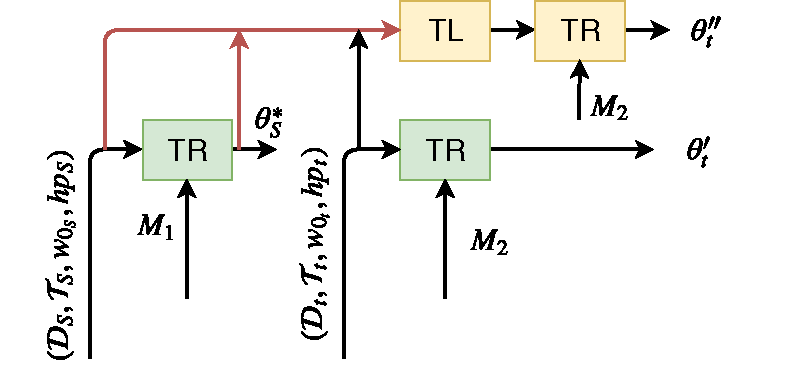
\includegraphics[width = 0.8\textwidth]{figures/transferLearning/TL.pdf}
    \caption[Η διαδικασία μετάδοσης γνώσης]{Η διαδικασία μετάδοσης γνώσης (TL) σε σχέση με την απλή εκπαίδευση (TR) και η σύγκριση της πορείας πληροφορίας. Η μεταβλητή $\theta^*_S$ είναι οι παράμετροι που επιστρέφει η εκπαίδευση στο αρχικό πεδίο ορισμού. Η μεταβλητή $\theta'_t$ είναι οι παράμετροι που επιστρέφει η εκπαίδευση στο τελικό πεδίο ορισμού χωρίς μετάδοση γνώσης. Η μεταβλητή $\theta''_t$ είναι οι παράμετροι που επιστρέφει η εκπαίδευση στο τελικό πεδίο ορισμού με χρήση μετάδοσης γνώσης.}
    \label{fig:TL}
\end{figure}
    


% η συνάρτηση πρόβλεψης έχει πιθανοτικά προσεγγιστεί ως $\hat{f}_s$, $\hat{f}_s(x) = M\left(x; W\right)$.
% Δηλαδή $ \mathtt{Prf}\left(T, \hat{f}\left(\mathcal{X}_{s_{test}}\right)\right) $.


% Δηλαδή $Pr\left(\abs{\hat{f}_s - f_s} >\delta\right) < \epsilon$ για κάποιο $\epsilon$ ικανά μικρό και $\epsilon(\delta) \downarrow$.
% Επίσης έστω ένα πεδίο ορισμού στόχου $\mathcal{D}_t$ και ένα έργο στόχος $ Τ_t $. Αν η συνάρτηση $f_t$ έχει πιθανοτικά προσεγγιστεί ως $\hat{f}_t$ λαμβάνοντας
% υπόψιν μόνο το πεδίο ορισμού στόχο και το έργο στόχο.
% Η μετάδοση γνώσης(Transfer Learning) είναι ένας αλγόριθμος ο οποίος έχει εν γένει είσοδο $(\mathcal{D}_s, T_s, \hat{f}_s, \mathcal{D}_t, T_t)$ και έξοδο μία


Στην παρούσα εργασία $ M_s = M_t = M$, δηλαδή χρησιμοποιείται το ίδιο μοντέλο στην αρχική και στην τελική εκπαίδευση, απλά οι παράμετροί τους δεν είναι ίδιες.

% transfer learning and multi-task learning
\section{Σχέση μετάδοσης γνώσης και μάθησης πολλαπλών έργων}
Η έννοια της μετάδοσης γνώσης είναι πολύ κοντινή με τη μάθηση πολλαπλών έργων (MTL) ταυτοχρόνως. Η MTL χρησιμοποιεί παραλληλισμό των έργων στο ίδιο πεδίο ορισμού. Με αυτό τον τρόπο μοιράζονται χαρακτηριστικά που εξάγονται στο ένα έργο και απαιτούνται στα υπόλοιπα. Στο τέλος αυτής της εκπαίδευσης μπορεί το μοντέλο να έχει καλύτερη επίδοση ακόμα και μόνο σε ένα έργο από ότι αν γινόταν εκπαίδευση μόνο σε αυτό ξεχωριστά. Οι λόγοι για τους οποίους συμβαίνει αυτό δε θα αναλυθούν, ωστόσο για παραπάνω διερεύνηση ο αναγνώστης παραπέμπεται στο \cite{43}. 

Η διαφορά με τη μετάδοση γνώσης είναι ότι η μετάδοση γνώσης λύνει το πρόβλημα σειριακά, μαθαίνοντας πρώτα τα χαρακτηριστικά τα οποία επιλύουν το πρώτο έργο και μετά μεταβαίνει στο επόμενο. Αν όλα τα έργα αφορούν το ίδιο πεδίο ορισμού, τότε η MTL είναι η προτεινόμενη λύση. Ωστόσο, δεν μπορεί να εφαρμοστεί όταν τα έργα αφορούν και διαφορετικά πεδία ορισμού. Αντίθετα, η μετάδοση γνώσης μπορεί να χρησιμοποιήσει χαρακτηριστικά από ένα έργο σε ένα πεδίο ορισμού και έργο $ \mathcal{D}_s, \mathcal{T}_s $ αντίστοιχα, προκειμένου να έχει καλύτερη επίδοση σε ένα πεδίο ορισμού και έργο $ \mathcal{D}_t, \mathcal{T}_t $.

% Present various scenarios
\section{Διάφορα σενάρια μετάδοσης γνώσης }
Παρακάτω δίνεται μία περίληψη των διαφόρων σεναρίων μετάδοσης γνώσης όπως αναφέρονται στα \cite{38} \cite{40}, αλλά με πιο σύγχρονα παραδείγματα.

\subsection{Επαγωγική μετάδοση γνώσης}
% \vspace{1ex}\\
{ \rule{1ex}{1ex} }%
\textit{Δοθέντος ενός αρχικού πεδίου ορισμού $\mathcal{D}_S$ με ένα αρχικό έργο $\mathcal{T}_S$ και ένα τελικό πεδίο ορισμού $\mathcal{D}_t$ με ένα τελικό έργο $\mathcal{T}_t$, η επαγωγική μετάδοση γνώσης αποσκοπεί στη βελτίωση της μάθησης της τελικής συνάρτησης ετικετοποίησης $f_t$ στο τελικό πεδίο ορισμού $\mathcal{D}_t$ χρησιμοποιώντας γνώση από τα $\mathcal{D}_S, \mathcal{T}_S$, όπου $\mathcal{T}_S \neq \mathcal{T}_t$.}

Στον παραπάνω ορισμό τα $\mathcal{D}_S$ και $\mathcal{D}_t$ μπορούν να είναι σχετικά. Βασιζόμενοι στο παραπάνω ορισμό, απαιτούνται μόνο λίγα ετικετοποιημένα δεδομένα για την πρόβλεψη της τελικής συνάρτησης ετικετοποίησης. Γενικά, πρόκειται για πληροφοριοδοτημένη άνευ επίβλεψης μετάδοση γνώσης, όπου εκεί βρίσκεται αρκετό ερευνητικό και πρακτικό ενδιαφέρον. Ωστόσο, υπάρχει και η περίπτωση να είναι Μη-Πληροφοριοδοτημένη άνευ επίβλεψης μετάδοση γνώσης.

% Ένα παράδειγμα της επαγωγικής μετάδοσης γνώσης περιγράφεται στο \cite{46}. Σε αυτό οι συγγραφείς λαμβάνουν ψυχομετρικά δεδομένα από ένα πείραμα εικονικής οδήγησης. Μετά από αυτό το πείραμα δημιουργήθηκε ένα μοντέλο για τη πρόβλεψη του βαθμού διέγερσης του ατόμου. Λαμβάνοντας όλα αυτά, δημιούργησαν ένα καινούριο μοντέλο για την πρόβλεψη της εγκεφαλικής δραστηριότητας και 

\subsubsection{Μεταφορά γνώσης από στιγμιότυπα}
Η μεταφορά στιγμιοτύπων για την επαγωγική μετάδοση γνώσης είναι αρκετά διαισθητική. Αν και η πλειονότητα των δεδομένων του αρχικού πεδίου ορισμού δεν μπορεί να χρησιμοποιηθεί απευθείας, υπάρχουν μέσα σε αυτά μέλη τους τα οποία μπορούν να χρησιμοποιηθούν μαζί με μερικά ετικετοποιημένα δεδομένα του τελικού πεδίου ορισμού.

Για παράδειγμα έχει προταθεί ο αλγόριθμος TrAdaBoost, ο οποίος είναι μία επέκταση του αλγορίθμου AdaBoost, προκειμένου να λύσει τα προβλήματα επαγωγικής μεταφοράς γνώσης. Ο TrAdaBoost υποθέτει ότι το αρχικό και το τελικό πεδίο ορισμού χρησιμοποιούν τις ίδιες ετικέτες και χαρακτηριστικά, αλλά οι κατανομές των δεδομένων στα δύο πεδία ορισμού είναι διαφορετικές. Επιπλέον, ο TrAdaBoost υποθέτει ότι λόγω της διαφοράς των κατανομών, μερικά από τα δεδομένα του αρχικού πεδίου ορισμού μπορεί να βοηθήσουν στην εκπαίδευση στο τελικό πεδίο ορισμού, αλλά μπορεί και να δυσχεραίνουν την εκπαίδευση.

Ο αλγόριθμος προσπαθεί να ζυγιάσει τα δεδομένα προκειμένου να μειώσει τα δεδομένα με αρνητική επίδραση στην εκπαίδευση και να ενισχύσει τα δεδομένα με θετική επίδραση στην εκπαίδευση στο τελικό πεδίο ορισμού. Σε κάθε επανάληψη του, ο TrAdaBoost εκπαιδεύει το βασικό ταξινομητή (συνάρτηση πρόβλεψης - μοντέλο) σε αυτό το ζυγιασμένο σύνολο δεδομένων. Ωστόσο, το σφάλμα υπολογίζεται μόνο στα δεδομένα του τελικού πεδίου ορισμού. Περεταίρω, ο TrAdaBoost ακολουθεί την ίδια στρατηγική με τον AdaBoost για την ανανέωση των λανθασμένα ταξινομημένων δεδομένων στο τελικό πεδίο ορισμού. Ωστόσο, χρησιμοποιείται διαφορετική στρατηγική για την ανανέωση των λανθασμένα ταξινομημένων δεδομένων στο αρχικό πεδίο ορισμού από το αρχικό μοντέλο. Στο \cite{63} δίνεται μία θεωρητική ανάλυση του αλγορίθμου TrAdaBoost.

\subsubsection{Μετάδοση γνώσης της αναπαράστασης χαρακτηριστικών}
Η προσέγγιση με τη μετάδοση της αναπαράστασης χαρακτηριστικών στο πρόβλημα της επαγωγικής μετάδοσης γνώσης σκοπεύει στην εύρεση αναπαραστάσεων χαρακτηριστικών για τη μείωση της απόκλισης των πεδίων ορισμού και του σφάλματος ταξινόμησης ή παλινδρόμησης του μοντέλου. Οι στρατηγικές για την εύρεση τέτοιων αναπαραστάσεων χαρακτηριστικών διαφέρουν μεταξύ τους ανάλογα με το αρχικό πεδίο ορισμού. Αν πολλά ετικετοποιημένα δεδομένα είναι διαθέσιμα στο πεδίο ορισμού, μπορούν να χρησιμοποιηθούν τεχνικές επιβλεπόμενης μάθησης για την εύρεση των χαρακτηριστικών. Αυτό είναι όμοιο με τη συνήθη μάθηση πολλαπλών έργων. Αν δεν υπάρχουν ετικετοποιημένα δεδομένα στο αρχικό πεδίο ορισμού, τότε θα πρέπει να χρησιμοποιηθούν μέθοδοι μη επιβλεπόμενης μάθησης, ώστε να κατασκευασθούν τα χαρακτηριστικά που χρειάζονται για αυτή την προσέγγιση.
\vspace{1em}

\textbf{Παράδειγμα 1ο}\\
Επιβλεπόμενη κατασκευή χαρακτηριστικών:

Όπως επισημάνθηκε παραπάνω οι μέθοδοι επιβλεπόμενης κατασκευής χαρακτηριστικών για την επαγωγική μετάδοση γνώσης είναι όμοιες με αυτές της μάθησης πολλαπλών έργων. Η βασική ιδέα είναι η εκμάθηση μίας χαμηλής διάστασης αναπαράστασης η οποία είναι κοινή μεταξύ σχετικών έργων. Επιπλέον, η καινούρια αυτή αναπαράσταση μπορεί να μειώσει το σφάλμα ταξινόμησης ή παλινδρόμησης του μοντέλου σε κάθε ένα από τα υποψήφια έργα.

Αυτή η προσέγγιση μπορεί να μελετηθεί και ως ένα πρόβλημα βελτιστοποίησης. Σε αυτό τα κοινά χαρακτηριστικά μπορούν να γίνουν γνωστά επιλύοντας το παρακάτω πρόβλημα:
$$
argmin \sum_{t \in \{\mathcal{T}_t, \mathcal{T}_S\} } {\sum_{i=1}^{n_t}} {L\left(y_{t_i}, \langle a_t, U^T x_{t_i} \rangle  \right) + \gamma \|A\|^{2}_{2,1} } 
$$
$$
U \in \mathbf{O}^d
$$
Στην παραπάνω εξίσωση  τα $\mathcal{T}_S$, $\mathcal{T}_t$ δηλώνουν το αρχικό και το τελικό έργο στα αντίστοιχα πεδία ορισμού. Επίσης ο $A = [a_s,a_t] \in R^{d\times2}$ είναι ένας πίνακας των παραμέτρων. Ο $U$ είναι ένας ορθογώνιος πίνακας $d \times d$ που απεικονίζει τα αρχικά δεδομένα υψηλής διάστασης σε αναπαραστάσεις χαμηλής διάστασης. Η νόρμα $(r, p)$ του $A$ ορίζεται ως $ \|A\|_{r,p} = \left( \sum_{i=1}^{d}{\| a^i\|_{p}^{r}} \right)^{\frac{1}{p}}$. Το πρόβλημα αυτό υπολογίζει τις αναπαραστάσεις $U^T X_T$, $U^S X_S$ και τις παραμέτρους, $A$ του μοντέλου ταυτοχρόνως. Το πρόβλημα βελτιστοποίησης μπορεί να μετατραπεί και σε ένα κυρτό πρόβλημα \cite{47}. Η λύση αυτή αναλύεται περισσότερο στο \cite{46}, ωστόσο όπως είναι εύληπτο από τον αναγνώστη θα μπορούσε να χρησιμοποιηθεί και ένα νευρωνικό δίκτυο (όχι απαραίτητα βαθύ) για την επίλυση του προβλήματος.
\vspace{1em}

\textbf{Παράδειγμα 2ο}\\
Άνευ επίβλεψης κατασκευή χαρακτηριστικών:

Ένα πολύ καλό παράδειγμα αυτής της προσέγγιση είναι ο νευρωνικός στατιστικολόγος όπως αναλύεται στο \cite{48}. 
Σύμφωνα με αυτούς, για να μεταφέρει μία μηχανή χαρακτηριστικά από το ένα σύνολο δεδομένων στο άλλο, θα πρέπει να καταλαβαίνει τις ομοιότητες. Για να το πράξει αυτό θα πρέπει να περιγράφει όλο το σύνολο δεδομένων και όχι να περιγράφει τα δεδομένα του απλά ως ανεπεξέργαστα σημεία. Προς αυτό το σκοπό χρησιμοποίησαν και επέκτειναν έναν μεταβλητό αυτόματο κωδικοποιητή \cite{49} για να υπολογίσει στατιστικά ενός συνόλου δεδομένων άνευ επίβλεψης. Οι στατιστικές αυτές μπορούν να χρησιμοποιηθούν για την ομαδοποίηση συνόλων δεδομένων και την ταξινόμηση άγνωστων μέχρι τώρα συνόλων δεδομένων. Ως εκ τούτου και το όνομα του αλγορίθμου, αφού μπορεί να εξάγει στατιστικές των συνόλων δεδομένων άνευ επίβλεψης χρησιμοποιώντας ένα νευρωνικό δίκτυο.

Μία άλλη γνωστή μέθοδος που αναλύει αυτή την περίπτωση είναι η χρήση μάθησης πολλαπλοτήτων.  Σε αυτή την εργασία \cite{50} προτείνεται μία προσέγγιση προκρουστικής ανάλυσης για την διάταξη των πολλαπλοτήτων, η οποία μπορεί να χρησιμοποιηθεί στην μετάδοση γνώσης μεταξύ προβλημάτων.

\subsubsection{Μετάδοση γνώσης των Παραμέτρων}
Οι περισσότερες μέθοδοι μεταφοράς παραμέτρων για την επαγωγική μετάδοση γνώσης υποθέτουν ότι δύο ξεχωριστά ή ίδια μοντέλα για σχετικά έργα θα πρέπει να μοιραστούν κάποιες παραμέτρους ή κατανομές υπερπαραμέτρων. Τα μοντέλα που βρίσκονται υπό αυτή τη μέθοδο συνήθως αφορούν πολλαπλά έργα. Αυτό βέβαια δεν προβάλει κάποιο πρόβλημα, απλά από το να παραλληλισθούν τα δύο πεδία ορισμού, τοποθετώντας ένα μοντέλο, λαμβάνεται το μοντέλο εκπαιδευμένο στο πρώτο πρόβλημα και χρησιμοποιούνται τα δεδομένα εστιάζοντας στην καλύτερη επίδοση του μοντέλου στο δεύτερο (τελικό) πρόβλημα. 

Σε αυτή την κατηγορία υπόκειται και το δίκτυο SqueezeDet. Αρχικά οι ερευνητές που το δημιούργησαν στο πρώτο κομμάτι του που είναι το SqueezeNet έλαβαν όλες τις παραμέτρους από προηγούμενη εκπαίδευση του SqueezeNet στο ImageNet. Αυτή είναι περίπου και η μέθοδος που ακολουθείται στην εργασία. Ωστόσο, αυτή έχει και ερωτήματα όπως: πώς να αποφασίσει κανείς πόσες παραμέτρους να λάβει από μία προηγούμενη εκπαίδευση, ποιες και πόσες παραμέτρους χρειάζεται να επαναεκπαιδεύσει, μήπως υπάρχει κάποια σχέση πως να αλλάξει τις υπερπαραμέτρους με βάσει την απόφαση λήψης των παραμέτρων; Αυτά και άλλα απαντώνται παρακάτω.


\subsection{Μεταγωγική μετάδοση γνώσης}
% \vspace{1ex}\\
{ \rule{1ex}{1ex} }%
\textit{Δοθέντος ενός αρχικού πεδίου ορισμού $\mathcal{D}_S$ με ένα αρχικό έργο $\mathcal{T}_S$ και ένα τελικό πεδίο ορισμού $\mathcal{D}_t$ με ένα τελικό έργο $\mathcal{T}_t$, η μεταγωγική μετάδοση γνώσης αποσκοπεί στη βελτίωση της μάθησης της τελικής συνάρτησης ετικετοποίησης $f_t$ στο τελικό πεδίο ορισμού $\mathcal{D}_t$ χρησιμοποιώντας γνώση από τα $\mathcal{D}_S, \mathcal{T}_S$, όπου $\mathcal{D}_S \neq \mathcal{D}_t$ και $ \mathcal{T}_s = \mathcal{T}_t $. Επιπλέον, θα πρέπει να υφίστανται κάποια μη ετικετοποιημένα δεδομένα στο τελικό πεδίο ορισμού στη διάρκεια της εκπαίδευσης.}

Η έννοια της μεταγωγικής μετάδοσης γνώσης δε θα πρέπει να συγχέεται με την έννοια της μεταγωγικής μάθησης όπου όλα τα δεδομένα ελέγχου πρέπει να είναι γνωστά κατά την εκπαίδευση, η οποία δεν επιτρέπει το μοντέλο να επαναχρησιμοποιηθεί για μελλοντικά δεδομένα. Για να εξάγει αποτελέσματα από τα καινούρια δεδομένα θα πρέπει να τα κατηγοριοποιήσει στις ίδιες κατηγορίες με όλα τα υπάρχοντα. Παρομοίως όμως με τη μεταγωγική μάθηση, στη μεταγωγική μετάδοση γνώσης υποτίθεται ότι υπάρχουν μη ετικετοποιημένα δεδομένα στο τελικό πεδίο ορισμού. 

Στον παραπάνω ορισμό της μεταγωγικής μετάδοσης γνώσης το αρχικό και το τελικό πεδίο ορισμού είναι τα ίδια, το οποίο συνεπάγεται ότι μπορεί η συνάρτηση πρόβλεψης του αρχικού προβλήματος να προσαρμοστεί για το δεύτερο και να χρησιμοποιηθεί για τα μη ετικετοποιημένα δεδομένα στο τελικό πεδίο ορισμού. Η προσαρμογή αυτή υπόκειται σε δύο περιπτώσεις: 1) Οι χώροι των των χαρακτηριστικών των δύο πεδίων ορισμού είναι διαφορετικοί $ \mathcal{X}_S \neq \mathcal{X}_t $ και 2) οι χώροι των χαρακτηριστικών των πεδίων ορισμού είναι ίδιοι, αλλά οι πιθανοτικές κατανομές είναι διαφορετικές: $ P\left(X_S\right) \neq P\left( X_t\right)$.  Αυτό είναι σχεδόν ίδιο με τις απαιτήσεις της προσαρμογής του πεδίου ορισμού και του προβλήματος της πόλωσης των δειγμάτων λόγω δειγματοληψίας.

\subsubsection{Μεταφορά γνώσης από στιγμιότυπα}
Οι προσεγγίσεις αυτού του τύπου βασίζονται κυρίως στη σημασία της δειγματοληψίας. Προκειμένου να δειχθεί η σημασία της επιλογής μεθόδου δειγματοληψίας, παρουσιάζεται το μεγαλύτερο πρόβλημα της μεταφοράς γνώσης από στιγμιότυπα που είναι η ελαχιστοποίηση του εμπειρικού ρίσκου. Γενικότερα, θα ήταν επιθυμητό οι βελτιστοποιημένες παραμέτροι $\theta^*$ του μοντέλου να είναι βελτιστοποιημένες ως προς το αναμενόμενο ρίσκο: 
$$
\theta^* = argmin_{\theta \in \Theta} E_{(x,y) \in P} \left[ l(x, y, \theta)\right]
$$
όπου $l(x, y, \theta)$ είναι η συνάρτηση σφάλματος η οποία εξαρτάται από την παράμετρο $\theta$. Ωστόσο είναι δύσκολο να εκτιμηθεί η κατανομή P. Για αυτό προτιμάται η ελαχιστοποίηση του εμπειρικού ρίσκου:
$$
\theta^* = argmin_{\theta \in \Theta} \frac{1}{n}\sum_{i=1}^{n} \left[ l(x_i, y_i, \theta)\right]
$$
όπου $n$ είναι το μέγεθος των δεδομένων προς εκπαίδευση.

Στη μεταγωγική μετάδοση γνώσης, σκοπός είναι η εύρεση ενός βέλτιστου μοντέλου για το τελικό πεδίο ορισμού δεδομένων ελαχιστοποιώντας το αναμενόμενο ρίσκο:
$$
\theta^* = argmin_{\theta \in \Theta} \sum_{(x,y) \in D_{d_t}} P\left(D_{d_t}\right) l(x, y, \theta)
$$

Αν δεν υπάρχουν ετικετοποιημένα δεδομένα στο τελικό πεδίο ορισμού δεδομένων, τότε θα πρέπει το μοντέλο να εξαχθεί από τα δεδομένα του αρχικού πεδίου ορισμού. Αν $ P(D_{d_S}) = P(D_{d_t}) $, τότε αρκεί να βελτιστοποιηθούν οι παράμετροι του μοντέλου όπως παρακάτω:
$$
\theta* = argmin_{\theta \in \Theta} \sum_{(x,y) \in D_{d_S}} P\left(D_{d_S}\right) l(x, y, \theta).
$$
Διαφορετικά αν $ P(D_{d_S}) \neq P(D_{d_t})$, θα πρέπει να αλλάξει το παραπάνω πρόβλημα βελτιστοποίησης, ώστε το μοντέλο που θα εξαχθεί από την εκπαίδευση να έχει δυνατότητα μεγάλης γενίκευσης στο τελικό πεδίο ορισμού. Η αλλαγή είναι η εξής:
$$
\theta^* = argmin_{\theta \in \Theta} \sum_{(x,y) \in D_{d_S}} \frac{P\left(D_{d_t}\right)}{P\left(D_{d_S}\right)} P\left(D_{d_S}\right) l(x, y, \theta)
$$
$$
	\approx argmin_{\theta \in \Theta} \sum_{i=1}^{n_S} \frac{P_t\left(x_{t_i}, y_{t_i}\right)}{P\left(x_{S_i}, y_{S_i}\right)}  l(x_{S_i}, y_{S_i}, \theta).
$$
Σε αυτή την αλλαγή τοποθετούνται διαφορετικές τιμές ποινής στα στιγμιότυπα $(x_{S_i}, y_{t_i})$ πολλαπλασιάζοντας τα με τα βάρη $\frac{P_t\left(x_{t_i}, y_{t_i}\right)}{P\left(x_{S_i}, y_{S_i}\right)}$. Κατά αυτό τον τρόπο εξάγεται ένα ακριβές μοντέλο για το τελικό πρόβλημα. Επιπρόσθετα, αφού τα έργα είναι κοινά, ισχύει $P\left( Y_t | X_t\right) = P\left(Y_S, X_S\right)$. Επομένως, ο λόγος των κατανομών μπορεί να προσεγγισθεί πιο εύκολα:
$$
 \frac{P\left(x_{t_i}, y_{t_i}\right)}{P\left(x_{S_i}, y_{S_i}\right)} =  \frac{P\left(x_{t_i}\right)}{P\left(x_{S_i}\right)}.
$$
Αν είναι δυνατόν να υπολογιστούν τα $\frac{P_t\left(x_{t_i}\right)}{P\left(x_{S_i}\right)}$ για κάθε στιγμιότυπο, τότε δύναται να επιλυθούν όλα τα προβλήματα που υπόκεινται στην κατηγορία της μεταγωγικής μετάδοσης γνώσης. Στη βιβλιογραφία υπάρχουν διάφοροι τρόποι για τον υπολογισμό του παραπάνω λόγου, ωστόσο ξεφεύγουν από το αντικείμενο αυτής της διπλωματικής.

Ένα άμεσα σχετιζόμενο παράδειγμα είναι η εργασία της \textit{brighter.ai} \cite{54} για τον εντοπισμό αντικειμένων σε εικόνες υπό διαφορετικές συνθήκες. Δηλαδή στα περισσότερα σύνολα δεδομένων για αλγορίθμους εντοπισμού, όπως και στις περισσότερες εκπαιδεύσεις δε λαμβάνονται υπόψη περιπτώσεις που οι καιρικές συνθήκες ή η ώρα της ημέρας δυσχεραίνουν την όραση. Έτσι οι περισσότεροι αλγόριθμοι δεν μπορούν να χρησιμοποιηθούν σε αυτές τις περιπτώσεις.

Για την αντιμετώπιση αυτού του του προβλήματος οι ερευνητές της \textit{brighter.ai} χρησιμοποίησαν 2 νευρωνικά δίκτυα τύπου GAN συνδεδεμένα σειριακά, ώστε να απεικονίσουν τα δεδομένα της μίας συνθήκης στην άλλη κρατώντας τη μορφή των αντικειμένων ώστε να μπορούν να εντοπιστούν. Αν η κατάσταση στην οποία ο αλγόριθμος είναι θεμιτό να λειτουργήσει είναι η νύκτα, τότε: Το πρώτο δίκτυο GAN μετατρέπει την εικόνα από νύκτα σε μέρα και το δεύτερο GAN από μέρα σε νύκτα. Οι ερευνητές τονίζουν τη σημασία του δευτέρου, ώστε να μπορεί να υπάρχει μία ισομορφική απεικόνιση. Επίσης, ως μετρική απόστασης της κατασκευασμένης εικόνας και της πραγματικής από τα δίκτυα GAN χρησιμοποιούν την ευκλείδεια απόσταση μεταξύ των χαρακτηριστικών που εξάγονται κάποιο νευρωνικό δίκτυο κατηγοριοποίησης (πιθανόν εκπαιδευμένο στο αρχικό πεδίο ορισμού) στο αρχικό πεδίο ορισμού και στο τελικό πεδίο ορισμού. Ως σφάλμα προσέγγισης χρησιμοποιούν την απόσταση των εικόνων σε κάθε GAN και ένα άλλο σχεδόν αμετάβλητο χαρακτηριστικό, ανάλογα με τις συνθήκη των εικόνων.Το ίδιο δίκτυο με το οποίο εξήχθησαν τα χαρακτηριστικά, μετά μπορεί να χρησιμοποιηθεί για τον εντοπισμό αντικειμένων.

\subsubsection{Μετάδοση γνώσης της αναπαράστασης χαρακτηριστικών}
Οι περισσότερες μελέτες μεταγωγικής μετάδοσης γνώσης  με τη μεταφορά χαρακτηριστικών, αφορούν αλγορίθμους μηχανικής μάθησης άνευ επίβλεψης. Για την καλύτερη κατανόηση αυτής της μεθόδου παρουσιάζονται δύο αλγόριθμοι.

1ος Αλγόριθμος \cite{52}\\
Νευρωνική μάθηση δομικής αντιστοιχίας:

Σε αυτή την εργασία οι συγγραφείς υιοθέτησαν τη μετάδοση γνώσης με δομική αντιστοιχία \cite{53}, αλλά προτίμησαν την αναζήτηση αυτής να την πραγματοποιήσουν με ένα πιο σύγχρονο τρόπο: τους νευρωνικούς αυτόματους κωδικοποιητές όπως εκθέτουν και οι ίδιοι. Το πρόβλημα βέβαια που επιλύουν αφορά την επεξεργασία της φυσικής γλώσσας (NLP). Αυτό βέβαια, δεν εμποδίζει την περίληψη αυτής της εργασίας στην παρούσα, αφού η αντιστοιχία μοντέλων που επιλύουν προβλήματα αυτού του τομέα με αυτά της τεχνητής όρασης είναι αρκετά συχνή. 

Αρχικά η προσέγγιση αυτή ξεχωρίζει τα χαρακτηριστικά σε αξονικά χαρακτηριστικά (ή χαρακτηριστικά άξονα) και στα υπόλοιπα. Ο διαχωρισμός αυτός γίνεται εκ των προτέρων, δηλαδή πριν την εφαρμογή του αλγορίθμου και αφορά το αρχικό πεδίο ορισμού. Τα αξονικά χαρακτηριστικά δίνονται ως υπέρ-παράμετροι στον αλγόριθμο και έπειτα αυτός αποφασίζει κατά πόσο εφικτή είναι η περιγραφή των υπολοίπων χαρακτηριστικών από αυτά τα αξονικά χαρακτηριστικά. 

Η αρχιτεκτονική της λύσης αναλύεται καλύτερα μέσω του Σχήματος \ref{fig:SCL_autoencoder}. Εκεί διακρίνονται οι διαφορές μεταξύ ενός απλού αποκωδικοποιητή και αυτής της μεθόδου. Όπως παρατηρείται και στην εργασία της νευρωνικής μάθησης δομικής αντιστοιχίας, είναι η πρώτη φορά που χρησιμοποιείται η αρχιτεκτονική του αυτόματου αποκωδικοποιητή για αυτό το σκοπό και για αυτό δεν χρησιμοποιήθηκε και κάποιος βαθύς κωδικοποιητής ή αποκωδικοποιητής.

\begin{figure}[H]
\centering
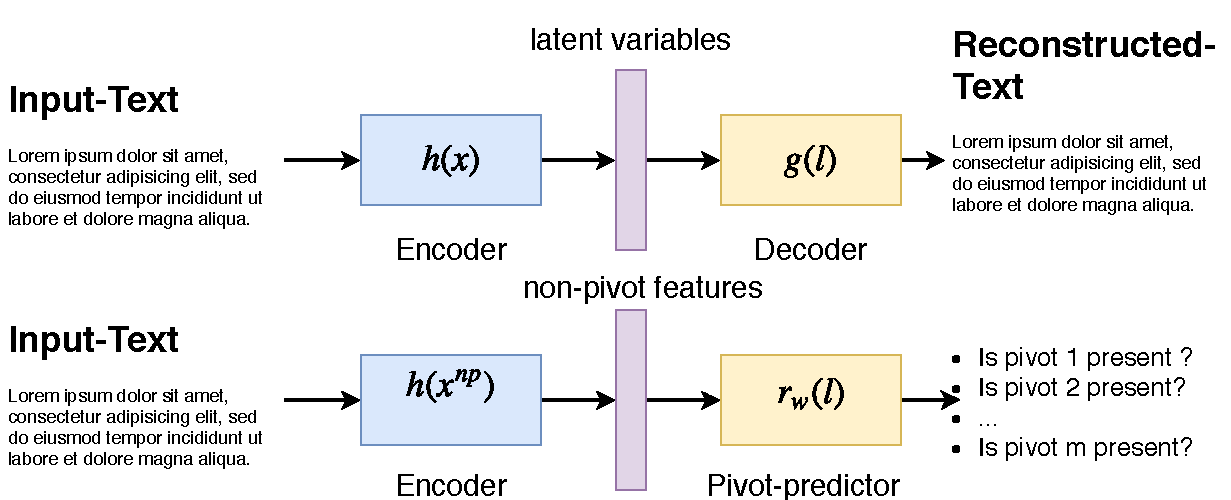
\includegraphics[width = \textwidth]{figures/transferLearning/SCL_autoencoder.pdf}
\caption[Αρχιτεκτονική νευρωνικής μάθησης δομικής αντιστοιχίας]{Στο πάνω μέρος της εικόνας βρίσκεται ένας απλός αυτόματος κωδικοποιητής. Στο κάτω μέρος της εικόνας βρίσκεται ο αυτόματος κωδικοποιητής αλλαγμένος στο κομμάτι του αποκωδικοποιητή όπως προβλέπει ο αλγόριθμος. Στο τέλος δε γίνεται ανακατασκευή της εισόδου, αλλά δίνεται η απάντηση αν κάποιο από τα αξονικά χαρακτηριστικά υπάρχει στην έξοδο του κωδικοποιητή. Το $x$ και το αποτέλεσμα της συνάρτησης $h(x^{np})$ είναι δυαδικά διανύσματα. Η βελτιστοποίηση γίνεται χρησιμοποιώντας τη συνάρτηση απόκλισης \textit{Kullback-Leibler}.}
\label{fig:SCL_autoencoder}
\end{figure}

2ος αλγόριθμος\\
Transfer Component Analysis (TCA):
Ο αλγόριθμος αυτός ουσιαστικά εξάγει χαρακτηριστικά από τα δύο πεδία ορισμού, θεωρώντας ότι όλα τα κοινά χαρακτηριστικά ανήκουν σε έναν αναπαραγόμενο χώρο πυρήνων Hilbert (RKHS). Τα δύο δεδομένα που λαμβάνει υπόψη του ο αλγόριθμος είναι ότι : $ P(X_S) \neq P(X_t)$ και $P(Y_S|X_S) = P(Y_t|X_t)$. Έπειτα θεωρώντας ότι υπάρχει μία λανθάνουσα απεικόνιση $\phi : \mathcal(X)\rightarrow mathcal(H)$ για τα $X_S$, $X_t$ η οποία είναι ισομορφισμός και ουσιαστικά δημιουργεί τα χαρακτηριστικά των δύο πεδίων ορισμού, ψάχνει αυτήν τη συνάρτηση $\phi$ η οποία ελαχιστοποιεί τη μετρική μέγιστης μέσης ασυμφωνίας(MMD):
$$
Dist(X_S’,X_t’) = \| \frac{1}{n_1} \sum_{i=1}^{n_1}\phi(x_{S_i}) -  \frac{1}{n_2} \sum_{i=1}^{n_2}\phi(x_{t_i}) \|_{\mathcal{H}}
$$
$$
\phi^* = argmin_{\phi} Dist(X_S’,X_t’)
$$
Σε αυτό το σημείο κάνει τη θεώρηση κλειδί αυτής της εργασίας, ότι $ P(Y_S|\phi(X_S)) = P(Y_t|\phi(X_t))$. Με αυτό και χρησιμοποιώντας το “κόλπο πυρήνα” $k(x_i,x_j) = \phi(x_i)^{T}\phi(x_j)$ οδηγείται στον υπολογισμό της μετρικής μέσω του πίνακα $K$:
$$
Dist(X_S’,X_t’) = tr(KL), \, K =\left[ \begin{matrix} K_{S,S} & K_{S,t}\\ K{t,S} & K_{t,t}\end{matrix}\right] , \, L_{ij} = \frac{1}{n_i n_j}, \, n_i = \left\{ \begin{matrix} n_1 \;\text{if}\. x_i \in X_S\\ n_2 \;\text{if}\; x_i \in X_t \end{matrix} \right.
$$

Βέβαια για τον υπολογισμό του K απαιτείται η λύση μέσω αλγορίθμων SDP και η μετέπειτα επεξεργασία της λύσης μέσω PCA για τη μείωση της διάστασης των χαρακτηριστικών. Αυτό οδηγεί σε μεγάλη πολυπλοκότητα και απώλεια πληροφορίας. Οπότε προτείνεται ο ορισμός ενός δευτέρου πίνακα μέσω της εξίσωσης $ K = \left(K K^{-1/2}\right) \left(K^{-1/2} K\right) $:
$$
\tilde{K} = \left(K K^{-1/2} \tilde{W}\right) \left(\tilde{W}^{T} K^{-1/2} K\right) = KWW^{T}K,\, W = K^{-1/2}\tilde{W} 
$$
οδηγώντας στη μετρική:
$$
Dist(X_S’, X_T’) = tr\left( (KWW^{T}K)L \right) = tr\left( W^{T}KLKW\right)
$$
Η οποία επιλύεται καλύτερα μέσω της αναζήτησης:
$$
W* = argmin_{W} \left[ tr(W^{T}W) + \mu tr\left( W^{T}KLKW\right) \right], \, W^{T}KLKW = I
$$
$$
H = I_{n_1+n_2} - \frac{1}{n_1+n_2} \mathbf{1}_{n_1+n_2,n_1+n_2}
$$
με $\mu$ ορισμένη ως παράμετρος συμβιβασμού. Το σύμβολο $\mathbf{1}_{n,m}$ είναι ένας πίνακας $n\times m$ με όλα τα στοιχεία του ίσα με 1. Η λύση αυτή δίνει πολυπλοκότητα $\mathrm{O}\left(m(n_1+n_2)^{2}\right)$.


\subsubsection{Μετάδοση γνώσης των Παραμέτρων}
Προφανώς στην μεταγωγική μετάδοση γνώσης δεν μπορεί να υπάρξει μετάδοση της γνώσης των παραμέτρων, διότι τα πεδία ορισμού είναι διαφορετικά. Για καλύτερη κατανόηση παρουσιάζεται ένα παράδειγμα: Αν ένα μοντέλο είναι εκπαιδευμένο σε δεδομένα εικόνων σε πολικές συντεταγμένες, τότε δεν μπορούν να χρησιμοποιηθούν οι παράμετροι του για την επίλυση του ίδιου προβλήματος σε καρτεσιανές, απλά μεταφέροντας κάποιες παραμέτρους. Ούτε βέβαια, μπορεί να βοηθηθεί γιατί τα μετέπειτα επίπεδα του μοντέλου με πιο υψηλής διάστασης χαρακτηριστικά βασίζονται στα προγενέστερα επίπεδα με χαμηλότερης διάστασης χαρακτηριστικά τα οποία είναι βασισμένα σε πολικές συντεταγμένες.

\subsection{Άνευ επίβλεψης μετάδοση γνώσης}
% \vspace{1ex}\\
{ \rule{1ex}{1ex} }%
\textit{Δοθέντος ενός αρχικού πεδίου ορισμού $\mathcal{D}_S$ με ένα αρχικό έργο $\mathcal{T}_S$ και ένα τελικό πεδίο ορισμού $\mathcal{D}_t$ με ένα τελικό έργο $\mathcal{T}_t$, η άνευ επίβλεψης μετάδοση γνώσης αποσκοπεί στη βελτίωση της μάθησης της τελικής συνάρτησης ομαδοποίησης ή περιγραφής των δεδομένων $f_t$ στο τελικό πεδίο ορισμού $\mathcal{D}_t$ χρησιμοποιώντας γνώση από τα $\mathcal{D}_S, \mathcal{T}_S$, όπου $\mathcal{T}_S \neq \mathcal{T}_t$ και τα $Y_S, Y_t$ είναι μη παρατηρήσιμα.}

Παρομοίως με τους ορισμούς που έχουν δοθεί στην απλή εκπαίδευση, η άνευ επίβλεψης μετάδοση γνώσης αφορά αρχικό και τελικό έργο χωρίς ορισμένες τις ετικέτες, δηλαδή χωρίς αυστηρά ορισμένη (ή είναι άγνωστη) συνάρτηση ετικετοποίησης. Ωστόσο υπάρχουν και άλλοι ορισμοί οι οποίοι πλαισιώνουν καλύτερα αυτό τον ορισμό υποκατηγοριοποιώντας τον σε συγκεκριμένα σενάρια. Σύμφωνα με τον Cook \cite{44} υπάρχουν τέσσερις κατηγορίες 
\begin{itemize}
    % \item IS: Πληροφοριοδοτημένη υπό επίβλεψη μετάδοση γνώσης, όπου η συνάρτηση ετικετοποίησης είναι γνωστή τόσο στο αρχικό έργο, όσο και στο τελικό.
    \item IU: Πληροφοριοδοτημένη άνευ επίβλεψη μετάδοση γνώσης, όπου η συνάρτηση ετικετοποίησης είναι γνωστή μόνο στο αρχικό έργο.
    \item US: Μη-πληροφοριοδοτημένη υπό επίβλεψη μετάδοση γνώσης, όπου η συνάρτηση ετικετοποίησης είναι γνωστή μόνο στο τελικό έργο.
    \item UU: Μη-Πληροφοριοδοτημένη άνευ επίβλεψη μετάδοση γνώσης, όπου η συνάρτηση ετικετοποίησης είναι άγνωστη τόσο στο αρχικό έργο, όσο και στο τελικό.
\end{itemize}

Διάφορες μέθοδοι έχουν αναπτυχθεί για την επίτευξη αποτελεσμάτων σε αυτές τις τέσσερις κατηγορίες. Η άνευ επίβλεψης μετάδοση γνώσης ονομάζεται και μάθηση μηδενικής λήψης (zero-shot learning). Οι εργασίες που αφορούν τη μάθηση μηδενικής λήψης προσπαθούν να απεικονίσουν το αρχικό πεδίο ορισμού στο τελικό και χρησιμοποιώντας αυτή την απεικόνιση να εκπαιδεύσουν ευκολότερα το μοντέλο στο τελικό πεδίο ορισμού. Για παράδειγμα αυτό θα μπορούσε να γίνει ακόμα και για ένα SVM \cite{45}. Παρόλα αυτά, σε όλες τις προσεγγίσεις συνεχίζουν να ισχύουν οι περιορισμοί των μεθόδων μάθησης άνευ επίβλεψης.

Αυτή η περίπτωση κυρίως περιλαμβάνει τη μεταφορά ομαδοποίησης από το αρχικό πεδίο ορισμού στο τελικό, ή την κατασκευή της τελικής ομαδοποίησης μέσω της τελικής. Η περίπτωση αναφέρεται απλά για πληρότητα. Για ένα παράδειγμα αυτής της μεθόδου ο αναγνώστης παραπέμπεται στον αλγόριθμο STC(αυτοδίδακτη ομαδοποίηση) \cite{53}.

\section{Μεταφερσιμότητα παραμέτρων νευρωνικών δικτύων επεξεργασίας εικόνας \cite{55}}
\label{section:transferability}
Όπως έχει παρουσιαστεί στην εργασία των ερευνητών του KTH \cite{56}, τα χαρακτηριστικά των εικόνων είναι αρκετά κοινά· επομένων μπορούν οι ίδιοι οι παράμετροι να μεταφερθούν από τον έναν αλγόριθμο στον άλλο με αρκετά καλό αποτέλεσμα και υποδιαιρώντας αρκετά τον χρόνο εκπαίδευσης. Επίσης, οι ίδιοι ερευνητές έδειξαν πως απλά προσθέτοντας ένα \textit{svm} στην κορυφή του δικτύου κρατώντας όλο το υπόλοιπο ίδιο και ανεκπαίδευτο στο τελικό πεδίο ορισμού, ήταν εφικτό τα ξεπεράσουν σχεδόν όλα τα αποτελέσματα των αλγορίθμων εκείνης της χρονικής περιόδου.

Όποτε γεννήθηκε ένα καινούριο ερώτημα στους ερευνητές, κατά πόσο αυτή η τεχνική είναι εφικτή, δηλαδή κατά πόσο είναι μεταφέρσιμοι οι παράμετροι των νευρωνικών δικτύων που επεξεργάζονται εικόνες \cite{55}. Όπως αναφέρουν ότι έχουν παρατηρήσει: τα πρώτα επίπεδα κάθε νευρωνικού δικτύου είναι ίδια, αφού πρόκειται για φίλτρα \textit{Gabor}· αυτό μάλιστα είναι συμβατό με την περίπτωσή μας διότι στις μετεκπαιδεύσεις του \textit{SqueezeDet} σε καινούρια σύνολα δεδομένων, τα αρχικά επίπεδα είχαν παραγώγους σφάλματος όπως φαίνεται στο Σχήμα \ref{fig:conv1_vs_conv12_biases_gradients}.

Προκειμένου να απαντήσουν οι ερευνητές στο ερώτημα, πραγματοποίησαν το εξής πείραμα: Λαμβάνοντας ως δίκτυο το AlexNet, πρώτα χώρισαν το ImageNet \cite{56}, με βάση τις κλάσεις του, σε δύο ξεχωριστά σύνολα δεδομένων(πεδία ορισμού) A, B και σε αυτά εκπαίδευσαν ξεχωριστά το δίκτυο, με αποτέλεσμα το δίκτυα Anet, Bnet αντίστοιχα. Ο χωρισμός έγινε με τέσσερις διαφορετικούς τυχαίους τρόπους. Έτσι δοκίμασαν την εκπαίδευση του AlexNet στο σύνολο δεδομένων B με τέσσερις διαφορετικούς τρόπους:

\begin{enumerate}

\item Στα $n$ πρώτα επίπεδα μεταφέρθηκαν παράμετροι από το Anet και αυτά έμειναν μη-εκπαιδεύσιμα, ενώ τα υπόλοιπα εκπαιδεύσιμα.

\item Στα $n$ πρώτα επίπεδα μεταφέρθηκαν παράμετροι από το Anet και όλα τα επίπεδα ήταν εκπαιδεύσιμα. Αυτό καλείται στην εργασία αυτή τελειοποίηση(\textit{fine-tuning}) των μεταφερόμενων παραμέτρων.

\item Στα $n$ πρώτα επίπεδα μεταφέρθηκαν παράμετροι από το Βnet και αυτά έμειναν μη-εκπαιδεύσιμα, ενώ τα υπόλοιπα εκπαιδεύσιμα.

\item Στα $n$ πρώτα επίπεδα μεταφέρθηκαν παράμετροι από το Βnet και όλα τα επίπεδα ήταν εκπαιδεύσιμα. Αυτό καλείται στην εργασία αυτή ως τελειοποίηση των μεταφερόμενων παραμέτρων.

\end{enumerate}

Οι δύο τελευταίες περιπτώσεις, έγιναν για να δείξουν ότι τα επίπεδα εξαρτώνται μεταξύ τους και κατά την εκπαίδευση έχουν εύθραυστη συν-προσαρμογή στα χαρακτηριστικά. Αυτό σημαίνει ότι για να γίνει σωστά η μετάδοση γνώσης δεν μπορεί να επιλεχθεί ο παραπάνω αριθμός $n$ χωρίς πρότερα να εξετασθούν οι αριθμοί $n-1$, $n+1$. Αυτό εξηγεί και την πτώση της έντονα κόκκινης γραμμής στο Σχήμα \ref{fig:net_transferability_results}. Τα αποτελέσματα που εξήγαγαν σε αυτό το Σχήμα φαίνεται να είναι θετικά για την περίπτωση της μεταφοράς με τελειοποίηση των παραμέτρων βελτιώνοντας την γενικότητα των χαρακτηριστικών. Επίσης, φαίνεται ότι τα τελευταία επίπεδα έχουν πιο ειδικά χαρακτηριστικά, ενώ τα πρώτα γενικότερα με αποτέλεσμα όταν το $n$ πλησιάζει μεγάλες τιμές η ακρίβεια του δικτύου στο σύνολο B να γίνεται αρκετά μικρότερη.

Σε επόμενο πείραμα οι ερευνητές προχώρησαν και χώρισαν το ImageNet πάλι σε δύο ξεχωριστά σύνολα A, B όπως πριν, αλλά με τη διαφορά ότι οι κλάσεις θα ήταν αρκετά διαφορετικές μεταξύ τους και όχι τυχαίες (για A είχαν το σύνολο των αντικειμένων κατασκευασμένων από τον άνθρωπο και για Β είχαν το σύνολο πραγμάτων που βρίσκονται στη φύση). Και από αυτό το πείραμα κατέληξαν ότι τα χαρακτηριστικά συνεχίζουν να είναι γενικά και ότι είναι προτιμότερο να χρησιμοποιήσει κανείς αυτά τουλάχιστον στα πρώτα επίπεδα από ότι να κάνει εξολοκλήρου την εκπαίδευση στο σύνολο B.


\begin{figure}
\centering
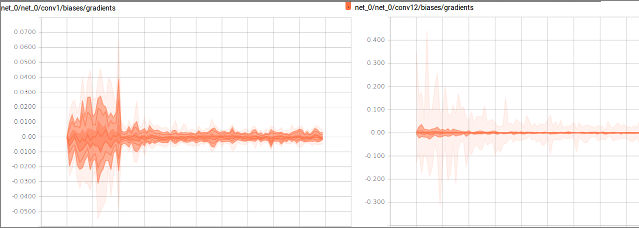
\includegraphics[width = \textwidth]{figures/transferLearning/conv1_vs_conv12_biases_gradients.png}
\caption[Οι κατανομές των παραμέτρων του πρώτου και του τελευταίου επιπέδου]{Η κατανομή της παραγώγου σφάλματος των παραμέτρων πόλωσης του πρώτου επιπέδου φαίνεται να έχει χαμηλότερα μέγιστα από ότι αυτές του τελευταίου επιπέδου κατά τάξη μεγέθους, δείχνοντας ότι το πρώτο επίπεδο του \textit{SqueezeNet}/\textit{SqueezeDet} είναι σχεδόν το ίδιο για τη μετεκπαίδευση στο τελικό πεδίο ορισμού PASCAL VOC2012 \cite{57} και στο αρχικό πεδίο ορισμού ImageNet.}
\label{fig:conv1_vs_conv12_biases_gradients}
\end{figure}

\begin{figure}
\centering
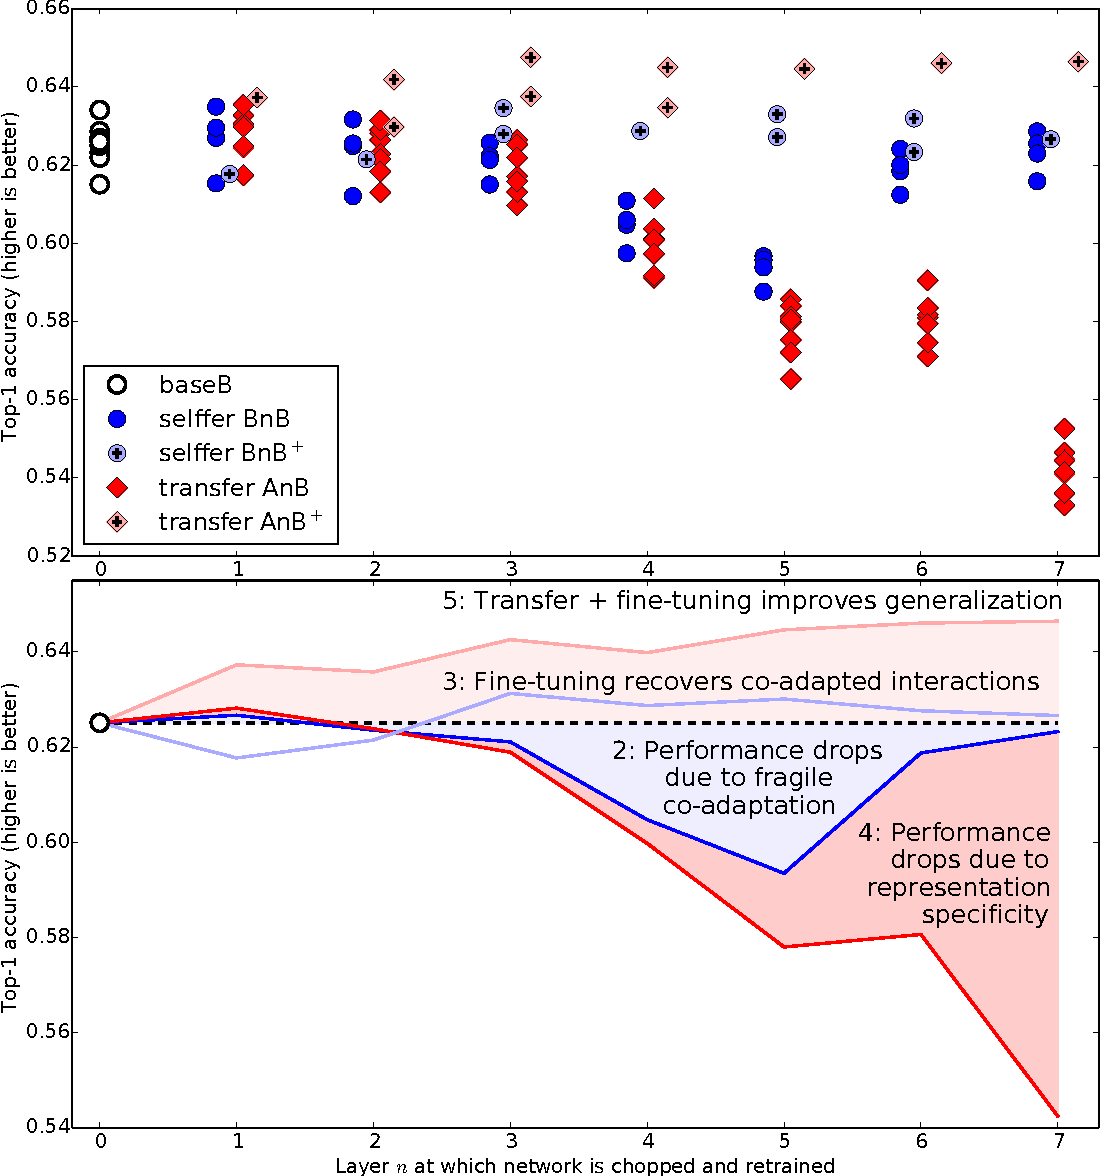
\includegraphics[width = \textwidth]{figures/transferLearning/net_transferability_results.png}
\caption[Τα αποτελέσματα της μετάδοσης γνώσης από το πείραμα μεταφερσιμότητα παραμέτρων]{Πάνω: Κάθε σήμανση στο σχήμα δείχνει τη μέση ακρίβεια στο σύνολο ελέγχου για το εκπαιδευμένο δίκτυο. Οι άσπροι κύκλοι στο $n=0$ δείχνουν την ακρίβεια του Bnet. Υπάρχουν οχτώ σημεία κάθε σήμανσης για κάθε $n$, διότι ελέγχθηκαν 4 διαφορετικοί τυχαίοι διαχωρισμοί του ImageNet. Κάθε κλειστός μπλε κύκλος παρουσιάζει την περίπτωση 3, ενώ κάθε μπλε κύκλος με σταυρό παρουσιάζει το 4. Κάθε κόκκινος ρόμβος παρουσιάζει την περίπτωση 1, ενώ κάθε κόκκινος ρόμβος με σταυρό παρουσιάζει την περίπτωση 2.  Κάτω: Οι γραμμές που συνδέουν τα μέσα του πάνω διαγράμματος για κάθε μία από τις 4 περιπτώσεις. Οι αριθμοί και τα κείμενα στην εικόνα επισημαίνουν το λόγο αυτής της συμπεριφοράς.}
\label{fig:net_transferability_results}
\end{figure}


\section{Αρνητική μετάδοση Γνώσης}
Ήδη από το πείραμα της προηγούμενης παραγράφου είναι κατανοητό ότι υπάρχουν όρια στη μεταφερσιμότητα των παραμέτρων. Όσο πιο διαφορετικά είναι το αρχικό με το τελικό πεδίο ορισμού, τόσο πιο δύσκολο είναι για το νευρωνικό να προσαρμοστεί. Μάλιστα, το πόσο μπορεί να προσαρμοστεί ένας αλγόριθμος έχει και θεωρητικό όριο στην περίπτωση που είναι μορφής Bayes με βάση την πολυπλοκότητα Kolmogorov \cite{61}. 

Αυτά όλα, είναι αρκετά για να φανταστεί κανείς την περίπτωση της αρνητικής μετάδοσης γνώσης, η οποία συμβαίνει “όταν η μεταφορά γνώσης από το αρχικό στο τελικό πρόβλημα προκαλεί μείωση της επίδοσης του αλγορίθμου” \cite{58}. Αυτό μπορεί να συμβαίνει για τρεις λόγους:
\begin{itemize}
\item Λάθος πληροφορία: Αν ο αλγόριθμος μετάδοσης γνώσης, αφαιρεί πληροφορία από το πρώτο πρόβλημα, την οποία θεωρεί ως επιβλαβούσα για την τελική εκπαίδευση, τότε η εκπαίδευση δεν είναι καλύτερη από την περίπτωση που ο αλγόριθμος εκπαιδευόταν μόνο στο τελικό πρόβλημα.
\item Επιλογή αρχικού έργου: Αν υπάρχει παραπάνω από μία επιλογή για το αρχικό σύνολο, ο αλγόριθμος μετάδοσης γνώσης υπάρχει περίπτωση να μην επιλέξει το βέλτιστο ή να διαλέξει να μην επιλέξει κανένα. Για την καλύτερη εικόνα επιλογής αρχικού προβλήματος, ο Eaton \cite{59} πρότεινε τη δημιουργία ενός γράφου όπου η απόσταση κάθε κόμβου από τους υπόλοιπους είναι ίση με μία μετρική μεταφερσιμότητα, όπως φαίνεται στο Σχήμα \ref{fig:transferability_graph}.
\item Ανομοιότητα στο αρχικό και το τελικό έργο: Αν αυτά τα δύο έργα είναι πολύ διαφορετικά, τότε υπάρχει μεγαλύτερο ρίσκο στην μεταγωγική μετάδοση γνώσης να προκληθεί μεγαλύτερο σφάλμα λόγω χρήσης της γνώσης του αρχικού προβλήματος. Αυτό συμβαίνει γιατί όσο πιο όμοια είναι δύο έργα, τόσο πιο κοινά είναι τα χαμηλών διαστάσεων χαρακτηριστικά τους \cite{60}.
\end{itemize}

\begin{figure}[H]
\centering
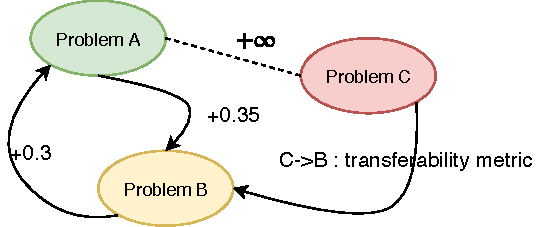
\includegraphics[width = \textwidth]{figures/transferLearning/transferability_graph.pdf}
\caption[Γράφος μεταφερσιμότητας]{Κατευθυνόμενος γράφος όπου κάθε κόμβος είναι ένα πρόβλημα με το δικό του έργο και το δικό του πεδίο ορισμού και κάθε ακμή έχει βάρος τη μετρική μεταφερσιμότητας από το αρχικό πρόβλημα προς το τελικό. Αυτός ο γράφος δεν παρουσιάζεται με αυτό το σχήμα στην εργασία \cite{59}, ωστόσο αυτό εννοείται. Επίσης επιβάλλεται να είναι κατευθυνόμενος λόγω της καταστροφικής \textit{λήθης}.}
\label{fig:transferability_graph}
\end{figure}

\section{Καταστροφική λήθη \cite{62}}
\label{section:catastrophicForgetting}
Τα νευρωνικά δίκτυα είναι κυρίως εμπνευσμένα από τη βιολογία του εγκεφάλου των θηλαστικών, ο οποίος εμπεριέχει νευρώνες οι οποίοι μαθαίνουν και εκπαιδεύονται σε καινούρια προβλήματα καθ’ όλη τη διάρκεια της ζωής του ατόμου. Αυτό σημαίνει ότι αν κάποιο άτομο μάθει να επιλύει ένα πρόβλημα δεν αποκλείει να μάθει την επίλυση ενός άλλου τουλάχιστον σε σύντομο χρονικό διάστημα. Δηλαδή, οι νευρώνες έχουν ελαστικότητα ως προς τη μάθηση.

Η παρατήρηση που έκαναν οι ερευνητές στο \cite{62} είναι ότι αυτό δε συμβαίνει μέχρι τώρα στις εκπαιδεύσεις των νευρωνικών δικτύων. Αυτό που συμβαίνει στην εφαρμογή της μετάδοσης γνώσης ή και στην απλή εκπαίδευση είναι ότι η βελτίωση της επίδοσης γίνεται μόνο για το αρχικό ή το τελικό πρόβλημα και αν έστω μία σειρά προβλημάτων όπως στο Σχήμα \ref{fig:transferability_graph} η διαδρομή $C\rightarrow B\rightarrow A$ δεν είναι εφικτή, διότι η μετάδοση γνώσης από το C στο B και η εκπαίδευση στο πρόβλημα B δεν επιτρέπουν το δίκτυο να ξανά-προσαρμοστεί στο A. Ωστόσο αν υπάρχουν δύο τέλειες λύσεις για τα προβλήματα A, B, τότε αυτές είναι κοντά όπως φαίνεται στο Σχήμα \ref{fig:elasticity_problem}, αλλά ο χώρος στον οποίο η μία λύση πρέπει να ανήκει για να είναι προσβάσιμη από την άλλη διαμέσου του μοντέλου είναι σε μία περιοχή γύρω από τη τέλεια λύση και όχι πάνω σε αυτή. 

Οπότε, είναι θεμιτό να υπολογιστεί αυτή η περιοχή. Ο υπολογισμός αυτής εξαρτάται από τα δεδομένα από ένα υποσύνολο  $\mathcal{D}$ του πεδίου ορισμού. Αν δηλαδή $\theta$ είναι οι παράμετροι του μοντέλου, τότε η πιθανότητα αυτή να είναι η τέλεια λύση για το πεδίο ορισμού $D$ είναι με βάση τον κανόνα Bayes:
$$
\\log p\left(\theta | \mathcal{D} \right) =  \log p\left( \mathcal{D}| \theta \right) + \log p\left(\theta \right) - \log p\left(\mathcal{D} \right)
$$
Οπότε αν συμβαίνει μεταφορά δεδομένων από το πρόβλημα A στο B, η πιθανότητα η $\theta$ να είναι η τέλεια λύση για κάποιο υποσύνολο δεδομένων $\mathcal{D}$:
$$
\log p\left(\theta | \mathcal{D} \right) =  \log p\left( \mathcal{D}_B| \theta \right) + \log p\left(\theta | \mathcal{D}_A\right) - \log p\left(\mathcal{D}_B \right)
$$
Η πραγματική πιθανότητα $ \log p\left(\theta | \mathcal{D}_A\right)$ είναι μη παρατηρήσιμη, οπότε αυτή προσεγγίζεται με μία κατανομή Gauss με μέση τιμή τις βέλτιστες παραμέτρους για το πρόβλημα A: $\theta^*_A$ και με τη διαγώνιο του πίνακα ακρίβειας ίση με τη διαγώνιο του πίνακα πληροφορίας Fisher. Το αποτέλεσμα είναι ότι προκειμένου να γίνουν οι νευρώνες πιο ελαστικοί κατά την εκπαίδευση στο πρόβλημα B μπορεί να χρησιμοποιηθεί η μετρική:
$$
\mathcal{L\left(\theta \right)} = \mathcal{L}_{B}\left(\theta \right) + \sum_{i} \frac{\lambda}{2} F_i\left( \theta_i - \theta^*_{A,i}\right)^2
$$
όπου $\mathcal{L}_{B}\left(\theta \right)$ είναι το σφάλμα κατά την εκπαίδευση στο πρόβλημα B, λαμβάνοντας μόνο υπόψη το πεδίο ορισμού και το έργο του B.


\begin{figure}[H]
\centering
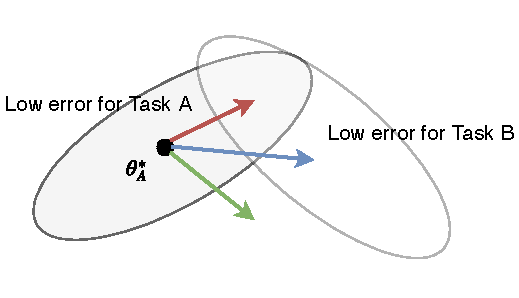
\includegraphics[width = \textwidth]{figures/transferLearning/elasticity_problem.pdf}
\caption[Αλγόριθμος EWC]{Ο αλγόριθμος EWC όπως προτείνεται στο \cite{62}. Προβάλλονται οι περιοχές στις οποίες η λύση είναι ικανοποιητική για τα δύο προβλήματα A,B. Επίσης, δείχνεται ποια η διαφορά μεταξύ των τριών σφαλμάτων: Με \textcolor{Maroon}{κόκκινο} η προτεινόμενη μετρική οδηγεί σε μία περιοχή των παραμέτρων η οποία έχει κοινά ικανοποιητικό σφάλμα. Με \textcolor{blue}{μπλε} η μετρική που δεν έχει βάρος ως προς το μέτρο των παραμέτρων εξέρχεται από την περιοχή της κοινά ικανοποιητικής λύσης. Με \textcolor{SeaGreen}{πράσινο} αν η μετρική σφάλματος λαμβάνει υπόψη το μέτρο των παραμέτρων χρησιμοποιώντας την ευκλείδεια απόσταση αυτών, μπορεί να οδηγηθεί εντελώς εκτός των δύο περιοχών.}
\label{fig:elasticity_problem}
\end{figure}

\section{Προσβασιμότητα}
 Με βάση τη θεωρία αυτομάτου ελέγχου, το παραπάνω πρόβλημα μπορεί να αντιστοιχηθεί σε πρόβλημα προσβασιμότητας. Η προσέγγιση αυτή γίνεται γιατί πιθανόν αυτή να συνδέει περισσότερο τη θεωρία που διδάσκεται ένας ηλεκτρολόγος μηχανικός με το αντικείμενο της μετάδοσης γνώσης. Οι ορισμοί από τη θεωρία προσβασιμότητας είναι οι εξής:
\vspace{1ex}\\
{ \rule{1ex}{1ex} }%
Δοθέντος ενός συστήματος $S(x,u,t)$ και μίας αρχικής κατάστασης $x_0$, η κατάσταση $x_f$ θεωρείται προσβάσιμη από την $x_0$ με είσοδο $u(t)$ αν το σύστημα εντός πεπερασμένου χρόνου $t_f$ μπορεί να μεταβεί από την κατάσταση $x_0$ στην κατάσταση $x_f$.

Επίσης, υπάρχει και ο χρήσιμος ορισμός του προσβάσιμου συνόλου:
\vspace{1ex}\\
{ \rule{1ex}{1ex} }%
Δοθέντος ενός συστήματος $S(x,u,t)$ και μίας αρχικής κατάστασης $x_0$, όλες οι καταστάσεις $x_j$ οι οποίες είναι προσβάσιμες δημιουργούν το προσβάσιμο σύνολο $R^{S}(x_0) = \{z\in X:x_{0}\rightarrow z \}$.
\vspace{1ex}\\
{ \rule{1ex}{1ex} }%
Αν $\Theta$ είναι η περιοχή με ικανοποιητική επίδοση, το αδιέξοδο σύνολο ορίζεται ως $N(S,\Theta) = \{z \in X: R^S(z)\cap \Theta \}$.

Στον παραπάνω ορισμό το αδιέξοδο σύνολο είναι δηλαδή οι καταστάσεις από τις οποίες δεν είναι εφικτή η μετάβαση στο σύνολο $\Theta$.
Έτσι, μπορεί να θεωρηθεί ότι η μετάδοση γνώσης είναι η χρήση προηγούμενων παραμέτρων ή ο μετασχηματισμός του χώρου εισόδου, ώστε το προσβάσιμο σύνολο να εμπεριέχει την περιοχή με το ικανοποιητικό σφάλμα ή να μετακινηθεί η αρχική θέση $x_0$ με αποτέλεσμα το καινούριο προσβάσιμο σύνολο να εμπεριέχει περιοχή με ικανοποιητικό σφάλμα. 

Στην κλασική μηχανική μάθηση όπου η εκπαίδευση γίνεται από την αρχή στο καινούριο πρόβλημα, δημιουργούνται τα εξής προβλήματα:
\begin{itemize}
    \item Έστω ότι γίνεται τυχαία επιλογή των παραμέτρων του μοντέλου $S$ με βάση κάποια συνάρτηση αθροιστικής κατανομής P. Αν η περιοχή με ικανοποιητική επίδοση είναι η $\Theta$, τότε η αρχική κατάσταση των παραμέτρων μπορεί να βρεθεί στο αδιέξοδο σύνολο $N(S,\theta)$, διότι εν γένει δεν ισχύει $P\left( N(S,\Theta)\right) = 0$. Οπότε, μπορεί να χρειαστούν αρκετές επαναλήψεις της εκπαίδευσης ώστε η αρχική κατάσταση να μη βρεθεί σε αυτό το σύνολο.
    \item Έστω ότι η επιλογή γίνεται από τον ερευνητή, τότε αυτός θα πρέπει να δοκιμάσει αρκετές τιμές, ώστε το σύνολο των αρχικών καταστάσεων που δοκίμασε να μην βρίσκεται εξολοκλήρου στο αδιέξοδο σύστημα.
\end{itemize}

 % Waiting for corrections
\chapter{Πειραματισμοί και αποτελέσματα}
\label{chapter:experiments}
\section{Το πρόβλημα και η προτεινόμενη λύση}
Οι αλγόριθμοι και τα παραδείγματα που αναφέρθηκαν στο κεφάλαιο \ref{chapter:tl} αφορούσαν αλγόριθμους οι οποίοι δεν είναι πραγματικού χρόνου και εμπεριέχουν μεγάλο πλήθος παραμέτρων και άρα μπορούν να χειριστούν περισσότερα χαρακτηριστικά των πεδίων ορισμού. Αντίθετα, οι αλγόριθμοι πραγματικού χρόνου μπορούν να χειριστούν μικρότερο πλήθος χαρακτηριστικών με αναμενόμενο αποτέλεσμα να δυσχεραίνεται η μεταφερσιμότητά τους.

Επιπλέον, τα νευρωνικά δίκτυα εντοπισμού αντικειμένων χρειάζεται να εντοπίζουν ένα αντικείμενο σε οποιαδήποτε θέση πάνω στην εικόνα. Στα δίκτυα πραγματικού χρόνου υπεύθυνος για τον εντοπισμό ενός αντικειμένου σε μία περιοχή είναι ένας νευρώνας. Αυτό επιταχύνει τον χρόνο εκτέλεσης του δικτύου, ωστόσο κάνει πιο δύσκολη την εκπαίδευση, αφού όλοι σχεδόν οι νευρώνες θα πρέπει να μπορούν να εντοπίσουν κάθε είδους αντικείμενο (που ανήκει στο σύνολο δεδομένων) στην περιοχή για την οποία είναι υπεύθυνοι. Αυτό συντελεί με τη σειρά του σε επιπλέον δυσκολία στη μεταφερσιμότητα κάνοντας τη σχεδόν αδύνατη, στα τελευταία επίπεδα του νευρωνικού.

Δεν υπάρχει κάποια αναφορά (εν γνώσει του συγγραφέα) σε δοκιμές για τη μεταφερσιμότητα των παραμέτρων νευρωνικών δικτύων εντοπισμού αντικειμένων που λειτουργούν σε πραγματικό χρόνο, εκτός από την πολύ πρόσφατη στο \cite{82}. Ωστόσο, σε αυτή την εργασία δε μελετάται με τον ίδιο τρόπο η μεταφερσιμότητα των παραμέτρων. Οπότε, πριν μπορέσει να υπάρξει οποιαδήποτε μελλοντική εφαρμογή θα πρέπει να γίνουν οι πειραματισμοί που παρουσιάζονται παρακάτω.

\section{Το πείραμα}
\label{section:TheExperiment}
Τα πειράματα που απαιτούνται είναι η χρήση ενός νευρωνικού δικτύου εντοπισμού αντικειμένων πραγματικού χρόνου για την πραγματοποίηση πρώτα του πειράματος που περιγράφεται στην ενότητα \ref{section:transferability}. Πρώτα, περιγράφονται τα θεωρητικά βήματα αυτού, μετά η διερεύνηση των αρχικών συνθηκών και τέλος τα αποτελέσματα. Σε μετέπειτα εργασία που περιγράφεται στο κεφάλαιο \ref{chapter:futures} κρίνεται σκόπιμη η υλοποίηση και του πειράματος που περιγράφεται στην ενότητα \ref{section:catastrophicForgetting}, ως μία άλλη σκοπιά στο πρόβλημα.

\subsection{Τα βήματα του πειράματος}
Σε αυτό το πείραμα παρουσιάζεται η συμπεριφορά της απλής επαγωγικής μετάδοσης γνώσης σε νευρωνικά δίκτυα εντοπισμού αντικειμένων πραγματικού χρόνου. Μέσω της συμπεριφοράς αυτής θα γίνει σαφές αν θα πρέπει να προτιμάται η μετάδοση γνώσης ή η μάθηση πολλαπλών έργων στα νευρωνικά δίκτυα εντοπισμού αντικειμένων πραγματικού χρόνου. Η μάθηση πολλαπλών έργων ωστόσο δεν μπορεί να γίνει για έναν οποιοδήποτε αριθμό κλάσεων αντικειμένων, διότι το δίκτυο για ικανά μεγάλο αριθμό μπορεί να σταματήσει να συμπεριφέρεται ως δίκτυο πραγματικού χρόνου.

Επιπρόσθετα, ήδη ο μεγάλος αριθμός κλάσεων δημιουργεί πρόβλημα στο SqueezeDet από άποψη της μνήμης που χρησιμοποιεί. Ο σκοπός δημιουργίας του δικτύου είναι αυτό να έχει μικρή μνήμη, ώστε να μπορεί να χρησιμοποιηθεί από μικρής ισχύος ενσωματωμένες συσκευές. Αν αυξηθεί ο αριθμός των κλάσεων κατά πολύ, το δίκτυο θα παύσει να λειτουργεί σωστά. Ο τύπος του μεγέθους του τελευταίου επιπέδου του SqueezeDet παρουσιάζεται στην παρακάτω εξίσωση:
$$
final\_layer\_shape = 3 \times 3 \times K(C+ 1 + 4)
$$
με $K$ τον αριθμό των υπεύθυνων νευρώνων ανά περιοχή πλέγματος και $C$ τον αριθμό των κλάσεων. Για αυτό το λόγο, όλες οι εκπαιδεύσεις θα πρέπει να περιορίζονται σε μικρό αριθμό κλάσεων.

Για την πραγματοποίηση του πειράματος επιλέχθηκαν τα σύνολα δεδομένων PASCAL\_VOC και KITTI. Αρχικά στο πείραμα χωρίζονται δύο σύνολα δεδομένων, ονόματι A, B, διαλέγοντας το KITTI ως το (Α) και το υποσύνολο του PASCAL\_VOC που εμπεριέχει τρεις (ιδανικά τυχαίες) κλάσεις (Β).

Τα βήματα που ακολουθούνται για την πραγματοποίηση του πειράματος είναι τα εξής:
\begin{enumerate}
\item Εκπαίδευση ολόκληρου του SqueezeDet στο υποσύνολο δεδομένων Α. Με το πέρας αυτής της εκπαίδευσης το στιγμιότυπο του δικτύου θα ονομάζεται δίκτυο A.
\item Εκπαίδευση ολόκληρου του SqueezeDet στο υποσύνολο δεδομένων B. Με το πέρας αυτής της εκπαίδευσης το στιγμιότυπο του δικτύου θα ονομάζεται δίκτυο B.

\item{Σε ένα καινούριο δίκτυο τύπου SqueezeDet αντιγράφονται τα $n$ πρώτα επίπεδα του δικτύου B σε αυτό και τα υπόλοιπα αρχικοποιούνται τυχαία με τη μέθοδο Xavier. Το δίκτυο εκπαιδεύεται στο σύνολο δεδομένων B. Τα $n$ πρώτα επίπεδα του δικτύου παραμένουν σταθερά. Με το πέρας αυτής της εκπαίδευσης το στιγμιότυπο του δικτύου θα ονομάζεται δίκτυο $BnB$.}

\item{Σε ένα καινούριο δίκτυο τύπου SqueezeDet αντιγράφονται τα $n$ πρώτα επίπεδα του δικτύου B σε αυτό και τα υπόλοιπα αρχικοποιούνται τυχαία με τη μέθοδο Xavier. Το δίκτυο εκπαιδεύεται στο σύνολο δεδομένων B. Τα $n$ πρώτα επίπεδα του δικτύου δεν παραμένουν σταθερά και εκπαιδεύονται μαζί με τα υπόλοιπα. Με το πέρας αυτής της εκπαίδευσης το στιγμιότυπο του δικτύου θα ονομάζεται δίκτυο $BnB^+$.}

\item{Σε ένα καινούριο δίκτυο τύπου SqueezeDet αντιγράφονται τα $n$ πρώτα επίπεδα του δικτύου A σε αυτό και τα υπόλοιπα αρχικοποιούνται τυχαία με τη μέθοδο Xavier \cite{77}. Το δίκτυο εκπαιδεύεται στο σύνολο δεδομένων B. Τα $n$ πρώτα επίπεδα του δικτύου παραμένουν σταθερά. Με το πέρας αυτής της εκπαίδευσης το στιγμιότυπο του δικτύου θα ονομάζεται δίκτυο $AnB$.}

\item{Σε ένα καινούριο δίκτυο τύπου SqueezeDet αντιγράφονται τα $n$ πρώτα επίπεδα του δικτύου A σε αυτό και τα υπόλοιπα αρχικοποιούνται τυχαία με τη μέθοδο Xavier. Το δίκτυο εκπαιδεύεται στο σύνολο δεδομένων B. Τα $n$ πρώτα επίπεδα του δικτύου δεν παραμένουν σταθερά και εκπαιδεύονται μαζί με τα υπόλοιπα. Με το πέρας αυτής της εκπαίδευσης το στιγμιότυπο του δικτύου θα ονομάζεται δίκτυο $AnB^+$.}

\end{enumerate}

Τα βήματα 3 έως 6 επαναλαμβάνονται για $n = 1,\hdots,11$ και για τρεις τυχαίους χωρισμούς του συνόλου δεδομένων σε υποσύνολα A, B. Η διαφορά μεταξύ των τεσσάρων εκπαιδεύσεων, παρουσιάζεται καλύτερα στο Σχήμα \ref{fig:tl_exp_config}, το οποίο περιγράφεται και στο \cite{55}. Η κάθε εκπαίδευση γίνεται με συμπερίληψη της μετρικής mAP όπως αναφέρεται στην ενότητα \ref{section:transferability}.


\begin{figure}
\centering
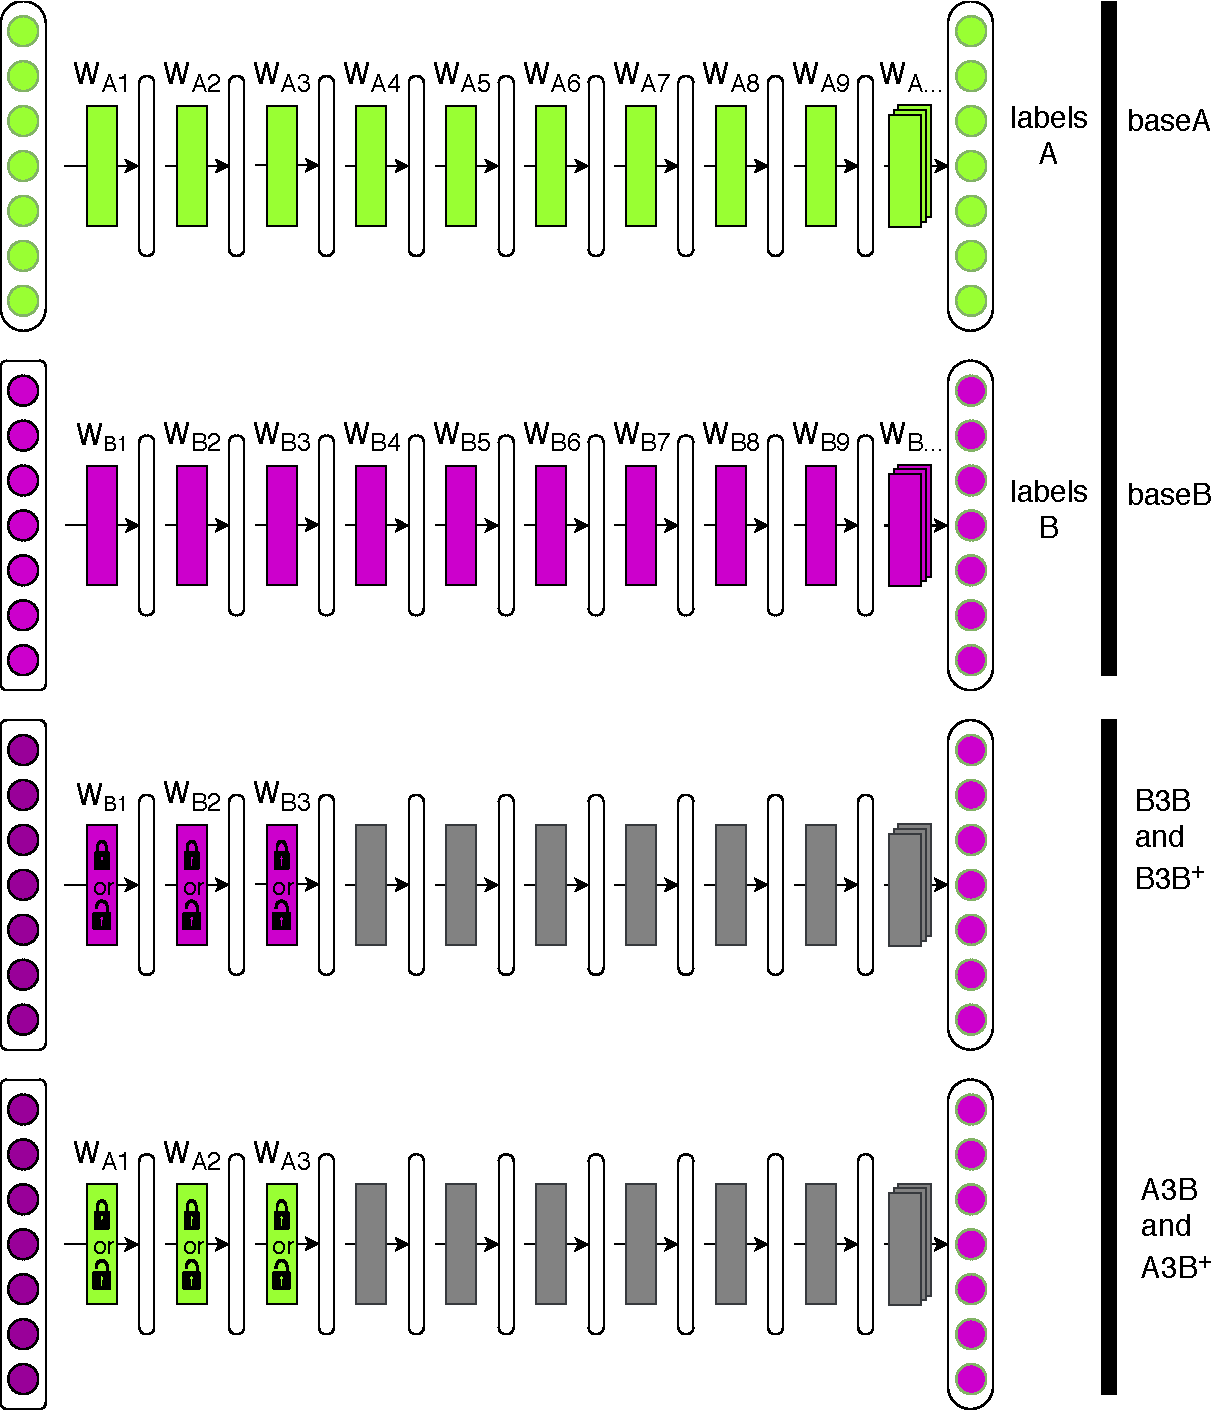
\includegraphics[width = \textwidth]{figures/experiments/tl_exp_config.pdf}
\caption[Οι τέσσερις διαφορετικές αρχικοποιήσεις του δικτύου]{Οι τέσσερις διαφορετικές αρχικοποιήσεις του δικτύου SqueezeDet κατά το πείραμα. Το \textcolor{myGreen}{πράσινο} χρώμα αναφέρεται στα δεδομένα που ανήκουν στο υποσύνολο δεδομένων A όπως και στο δίκτυο A. Ενώ το \textcolor{magenta}{μωβ} χρώμα αναφέρεται στα δεδομένα που ανήκουν στο υποσύνολο δεδομένων B και στο δίκτυο B. Τα ορθογώνια με \textcolor{myGrey}{γκρι} χρώμα δείχνουν τα επίπεδα στα οποία οι παράμετροί τους αρχικοποιούνται με τυχαίες τιμές χρησιμοποιώντας τη μέθοδο Xavier.}
\label{fig:tl_exp_config}
\end{figure}

\subsection{Εκπαίδευση στο σύνολο δεδομένων A}
\label{subsection:Atrain}
Ως σύνολο δεδομένων Α ελήφθη το σύνολο δεδομένων του KITTI, το οποίο είναι αρκετά μεγάλο και είχε σίγουρα ικανοποιητικά αποτελέσματα για το SqueezeDet. Οι κλάσεις στις οποίες εκπαιδεύτηκε το δίκτυο είναι οι "car", "pedestrian", "cyclist" όπως και στην αρχική εργασία. Η διαφορά στο μέγεθος των εικόνων των δύο συνόλων δεδομένων θα οδηγήσει στην ανικανότητα μελέτης του τελευταίου επιπέδου του νευρωνικού ως προς τη μετάδοση γνώσης. Ωστόσο, το τελευταίο επίπεδο θεωρείται σύμφωνα με το αρχικό πείραμα ότι θα δώσει υπερβολικά χαμηλής απόδοσης αποτελέσματα για τα $AnB$ και $AnB^+$. Επιπλέον, δεν μπορεί να γίνει κάποια σύγκριση αν ο παραπάνω αριθμός $n$ είναι ίσος με όλα τα επίπεδα του νευρωνικού, διότι πρόκειται για εκφυλισμένη περίπτωση.

Η εκπαίδευση έγινε στο KITTI για $35000$ επαναλήψεις δίνοντας τα αποτελέσματα που διακρίνονται στο Σχήμα \ref{fig:Atrain}. Η εκπαίδευση δεν προχώρησε σε παραπάνω βήματα, διότι αυτό θα σήμαινε υπέρ-προσαρμογή του δικτύου στο σύνολο δεδομένων του KITTI.

\begin{figure}
\centering
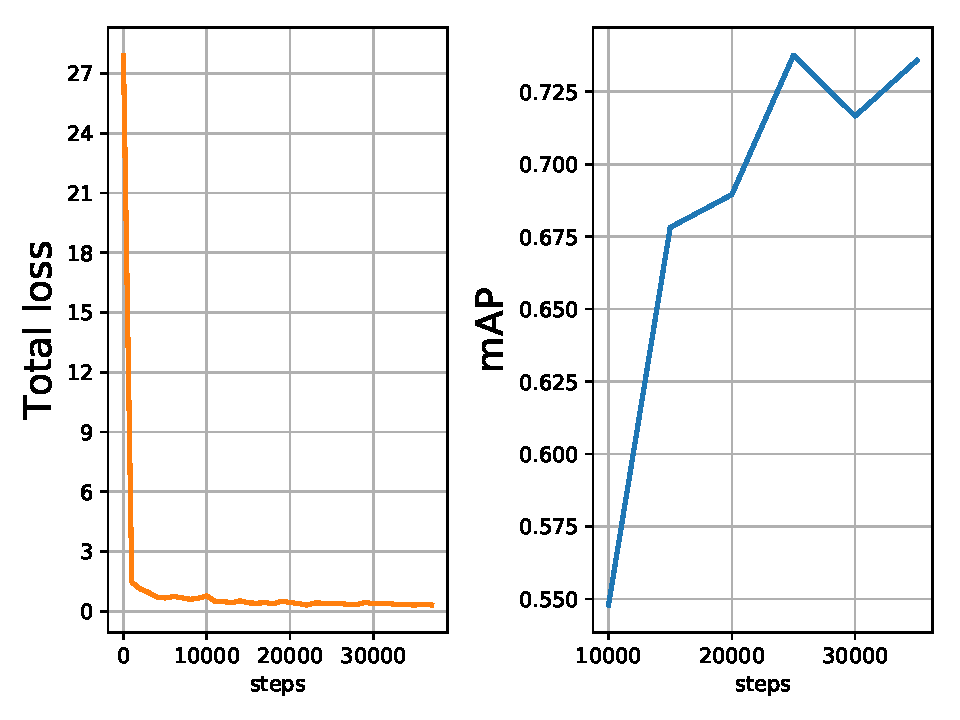
\includegraphics[width = \textwidth]{figures/experiments/Atrain.pdf}
\caption[Η εκπαίδευση του SqueezeDet στο σύνολο δεδομένων A, με χρήση βαρών του ImageNet]{Η εκπαίδευση του SqueezeDet στο σύνολο δεδομένων A (KITTI) με χρήση βαρών του ImageNet. Η χρήση μετάδοσης γνώσης παραμέτρων σε αυτή την εκπαίδευση δεν έχει καμία επιρροή στο πείραμα. Το μέγιστο mAP το οποίο μπορεί να επιτευχθεί δε φαίνεται σε αυτή την εκπαίδευση καθότι θα έπρεπε τα βήματα να είναι ακόμα $15000$ το οποίο μπορεί να οδηγήσει και σε υπέρ-προσαρμογή.}
\label{fig:Atrain}
\end{figure}

\subsection{Εκπαίδευση στο σύνολο δεδομένων Β}
\label{subsection:Btrain}
Το σύνολο δεδομένων Β προέρχεται από το σύνολο δεδομένων PASCAL\_VOC. Η συνολική εκπαίδευση στο συνολικό σύνολο δεδομένων φάνηκε αδύνατη ως επιλογή διότι το SqueezeDet δεν είναι υλοποιημένο με το σκεπτικό να αναγνωρίζει ένα μεγάλο σύνολο δεδομένων, άλλωστε αυτό έδειξαν και τα πειράματα κατά τη συνολική εκπαίδευση του δικτύου σε αυτό το σύνολο δεδομένων όπως φαίνεται και στο Σχήματα \ref{fig:Btrain1}, \ref{fig:Btrain2}. Οπότε, για την εύρεση των υπερπαραμέτρων και του βέλτιστου υποσυνόλου χρειάστηκε να γίνουν αρκετές δοκιμές επιλογής τους. Το σύνολο που επιλέχθηκε ως B ήταν το σύνολο που έχει ως κλάσεις τις "bicycle", "bus", "dog", στο οποίο μετά από εκπαίδευση το δίκτυο επιτυγχάνει mAP $40\%$. Μάλιστα, μετά τις $20000$ επαναλήψεις λάμβανε χώρα το φαινόμενο της υπέρ-προσαρμογής, οπότε και προτείνεται στο συνολικό πείραμα ο πειραματισμός με μόνο $30000$ επαναλήψεις ανά επί μέρους επανεκπαίδευση.

Προκειμένου να επιταχυνθούν οι δοκιμές μεταφέρθηκαν οι παράμετροι του squeezeNet από προηγούμενη εκπαίδευση του στο ImageNet. Αρχικά, επιλέχθηκε ένα τυχαίο σύνολο με κλάσεις τις "aeroplane", "bicycle", "bird" και δοκιμάστηκε η εύρεση τυχαίων υπερπαραμέτρων. Οι μετρήσεις σε αυτό το πρώτο υποσύνολο δεν ήταν καθόλου ικανοποιητικές, καθότι στην καλύτερη περίπτωση το mAP στο σύνολο δεδομένων ελέγχου ήταν $24\%$. Στη συνέχεια έγιναν δοκιμές και σε άλλα τυχαία επιλεγμένα σύνολο οι οποίες φαίνονται στον Πίνακα \ref{table:subsetSearch}. Όλες οι μετρήσεις αφορούν τις πρώτες $45000$ επαναλήψεις κάθε εκπαίδευσης. Δοκιμάστηκε η εκπαίδευση με τη μέθοδο Adam \cite{19}, ωστόσο αυτή είχε ακόμα χειρότερη γενίκευση ($mAP=0.001$) από ότι η μέθοδος Momentum \cite{81} που χρησιμοποιείται από την αρχική έκδοση του SqueezeDet.

\begin{figure}
\centering
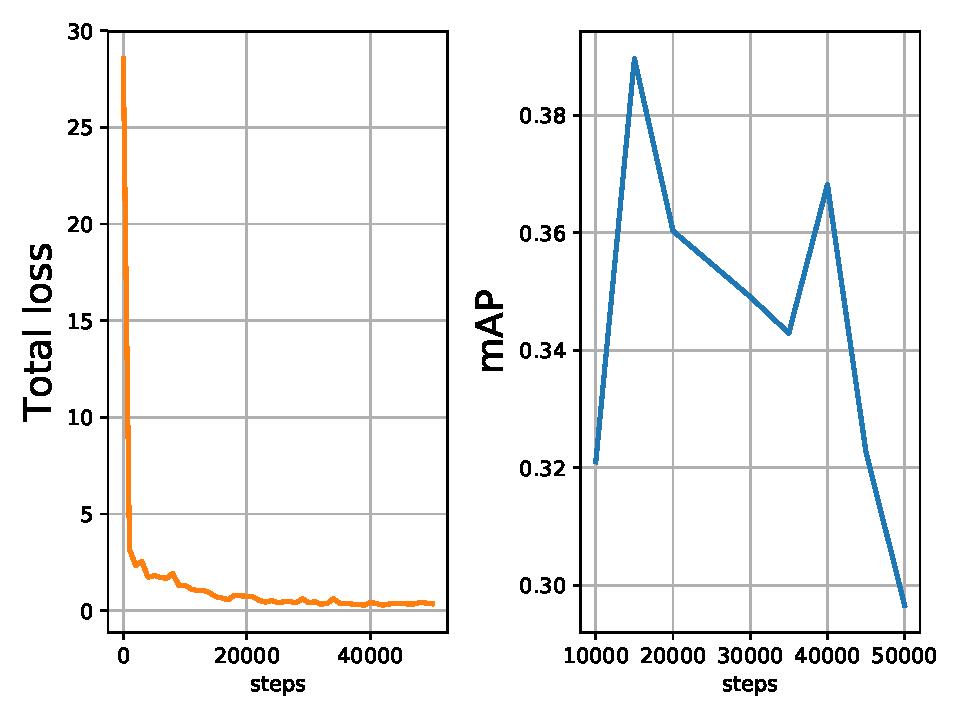
\includegraphics[width = \textwidth]{figures/experiments/Btrain1.pdf}
\caption[Η εκπαίδευση του SqueezeDet στο σύνολο δεδομένων B, με χρήση βαρών του ImageNet]{Η εκπαίδευση του SqueezeDet στο σύνολο δεδομένων B με χρήση βαρών του ImageNet. Η χρήση των βαρών του ImageNet στα επίπεδα του SqueezeDet δείχνει την αρκετά καλύτερη συμπεριφορά την οποία θα μπορούσε να έχει το δίκτυο αν ιδανικά εκπαιδευόταν για πάνω από χίλιες εποχές και σε περισσότερα δεδομένα.}
\label{fig:Btrain1}
\end{figure}

\begin{figure}
\centering
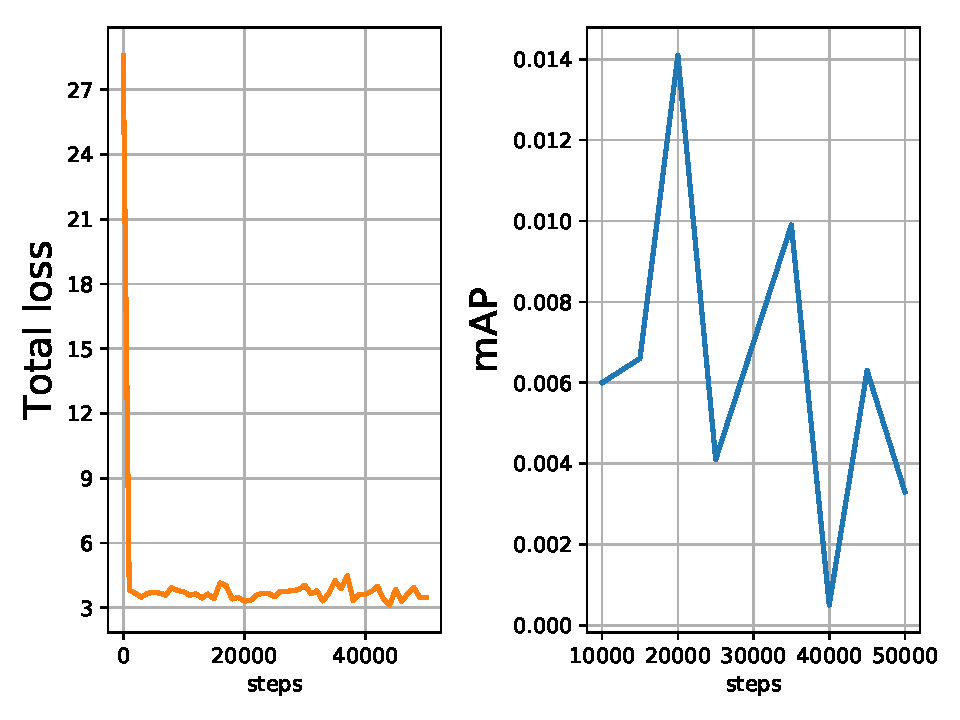
\includegraphics[width = \textwidth]{figures/experiments/Btrain2.pdf}
\caption[Η εκπαίδευση του SqueezeDet στο σύνολο δεδομένων B, χωρίς τη χρήση βαρών του ImageNet]{Η εκπαίδευση του SqueezeDet στο σύνολο δεδομένων B χωρίς τη χρήση βαρών του ImageNet. Η εκπαίδευση κατά αυτό τον τρόπο προφανώς δεν μπορεί να τελειώσει εντός $40000$ επαναλήψεων και θα χρειαστεί μέρες για να φτάσει στο ίδιο αποτέλεσμα. Επίσης, απαιτούνται περισσότερα δεδομένα (όπως παρουσιάζεται παρακάτω) για την επίτευξη ικανοποιητικού mAP. Αυτά όλα βέβαια με την προϋπόθεση πως η εντελώς τυχαία επιλογή παραμέτρων δεν αποκλείει την προσβασιμότητα στις ιδανικές παραμέτρους.}
\label{fig:Btrain2}
\end{figure}

\begin{table}[]
\centering
\caption{Εκπαιδεύσεις σε τυχαία επιλεγμένα υποσύνολα του PASCAL\_VOC.}
\label{table:subsetSearch}
\begin{tabular}{|l|l|}
\hline
\textbf{Υποσύνολο} & βέλτιστο \textbf{mAP} \\ \hline
"aeroplane", "bicycle", "bird" & $24\%$ \\ \hline
"bicycle", "bus", "car" &  $35\%$\\ \hline
"cat", "dog", "bird" & $24\%$  \\ \hline
"cat", "dog", "person" & $34\%$ \\ \hline
"cat", "dog", "bicycle" & $21\%$ \\ \hline
"bicycle", "bus", "dog" & $40\%$ \\ \hline
\end{tabular}
\end{table}
Ένας από τους λόγους για τους οποίους οι εκπαιδεύσεις δεν αποδίδουν υψηλή μετρική mAP είναι ότι οι εικόνες που εισάγονται στο νευρωνικό κατά το πλείστον δεν εμπεριέχουν όλες τις κλάσεις ή πάνω από μία κλάση αντικειμένων.

Τέλος, για να συμπληρωθεί η επιλογή των υπερπαραμέτρων, το μέγεθος της εικόνας που εισάγεται στο πρώτο επίπεδο του δικτύου είναι $(h,w) = (334, 500)$. Η επιλογή αυτή έγινε μετά από στατιστική ανάλυση του συνόλου δεδομένων και βρέθηκε πως ο μέσος όρος των μεγεθών των εικόνων βρισκόταν σε αυτό το σημείο. Επίσης, δοκιμάστηκαν τιμές αρκετά μεγαλύτερες αλλά και σε γειτονικά σημεία και βρέθηκε ότι αυτό το μέγεθος εικόνας δίνει το καλύτερο δυνατό mAP.

\subsection{Τελικά αποτελέσματα}
\label{section:grantExpRes}
Τα τελικά αποτελέσματα του πειράματος φαίνονται στο Σχήμα \ref{fig:grantExpRes} και με λογαριθμικό σκέλος της μετρικής mAP στο Σχήμα \ref{fig:grantExpResLog}. Με μία πρώτη ματιά το πείραμα φαίνεται να μην πέτυχε ως προς τη μεταφερσιμότητα των παραμέτρων. Λόγω αυτού, εξετάστηκε το ενδεχόμενο ο αριθμός των επαναλήψεων να ήταν πολύ μικρός. Οπότε, έγινε επανάληψη των πειραμάτων του δικτύου $AnB^+$ χρησιμοποιώντας $100000$ επαναλήψεις, δηλαδή περίπου $1800$ εποχές.

Η καινούρια επανάληψη των πειραμάτων του $AnB^+$ έδειξε πως η μετρική mAP δεν μπορούσε να βελτιωθεί με τη χρήση περισσότερων εποχών. Οπότε, συνεπάγεται ότι και τα τελικά αποτελέσματα του $AnB$ είναι σωστά, αφού αυτά θα έπρεπε να είναι το πολύ όσο οι τιμές των $AnB^+$. Επίσης, τα αποτελέσματα $BnB, BnB^+$ δοκιμάστηκαν ως προς τις $65000$ επαναλήψεις στα σημεία $n=4$ και $n=5$ δίνοντας ξανά τα ίδια αποτελέσματα. Άρα και οι επανεκπαιδεύσεις των δικτύων $BnB, BnB^+$ δεν απαιτούν παραπάνω επαναλήψεις για να πετύχουν καλύτερη μετρική mAP στο σύνολο ελέγχου. 

Επομένως, κύριο πρόβλημα δεν είναι ο μικρός αριθμός των επαναλήψεων, αλλά μάλλον ο μικρός αριθμός παραδειγμάτων για τη μετεκπαίδευση του δικτύου στο σύνολο Β. Ο μικρός αυτός αριθμός οδηγεί ταυτόχρονα και στην ανικανότητα εκπαίδευσης του δικτύου όπως στην παράγραφο \ref{subsection:Btrain} χωρίς τη μεταφορά παραμέτρων από το ImageNet. Οπότε, η μετεκπαίδευση αυτή παρουσιάζει ένα παράδειγμα στο οποίο οι παράμετροι της εκπαίδευσης του SqueezeNet, που αποτελεί τον κύριο κορμό του SqueezeDet, εκπαιδευμένες στο ImageNet είναι πιο γενικές από τις οποιεσδήποτε παραμέτρους του SqueezeDet μετά από εκπαίδευση του στον εντοπισμό αντικειμένων ενός συνόλου δεδομένων, διότι σε αυτό το σύνολο χρειάζεται οι παράμετροι του SqueezeDet να προσαρμοστούν παραπάνω για τον εντοπισμό συγκεκριμένων αντικειμένων.

Γνωρίζοντας ότι η μετεκπαίδευση δεν εξαρτάται από επιπλέον επαναλήψεις και με κάθε επιφύλαξη ότι στο σύνολο δεδομένων B μπορεί να γίνει εκπαίδευση όπως αυτή δοκιμάστηκε στην παράγραφο \ref{subsection:Btrain}, μπορεί να εξηγηθεί η συμπεριφορά του Σχήματος \ref{fig:grantExpRes} και του Σχήματος \ref{fig:grantExpResLog}. Στο σύνολο που επιλέχθηκε, το δίκτυο παρουσιάζει αρκετά εύθραυστη συν-προσαρμογή για αυτό και τα $7$ πρώτα επίπεδα θα πρέπει να είναι εκπαιδεύσιμα ώστε να μπορέσει να γίνει καλύτερη μετεκπαίδευση και να λειτουργήσει η μεταφορά των παραμέτρων. Επίσης, σε αυτό το σημείο δε βοηθάει ιδιαίτερα η τελειοποίηση (\textit{fine tuning}) καθότι έχει σχεδόν τα ίδια αποτελέσματα. Μάλιστα, αυτά είναι λίγο χειρότερα για τα πρώτα επίπεδα όπως παρουσιάζεται στο Σχήμα \ref{fig:grantExpResLog}. 

Αν τα αποτελέσματα των μετεκπαιδεύσεων των δικτύων $BnB^+$ ήταν καλύτερα από τα $BnB$, τότε θα υπήρχε λόγος σημαντικής βελτίωσης των αποτελεσμάτων στα δίκτυα $AnB^+$ από ότι στα $AnB$. Ωστόσο, τα πειράματα δείχνουν το αντίθετο που σημαίνει ότι η τελειοποίηση (\textit{fine tuning}) δεν πετυχαίνει τίποτα παραπάνω. Βέβαια, εξαιρούνται οι περιπτώσεις για $n \geq 7$, στις οποίες όμως η συμπεριφορά βελτιώνεται το πολύ κατά $1\%$. Για τη μετεκπαίδευση αυτό σημαίνει ότι ακόμα και η καλύτερη περίπτωσή μετάδοσης γνώσης με τελειοποίηση αποτυχαίνει να ανακτήσει υψηλότερη μετρική mAP στο σύνολο ελέγχου.

Όσον αφορά τα δίκτυα $BnB$, οι επανεκπαιδεύσεις των δικτύων αυτών έχουν χειρότερη μετρική mAP στο σύνολο ελέγχου σε όλες τις περιπτώσεις. Η εξήγηση είναι ότι πέρα από ότι το δίκτυο έχει πολλά εύθραυστα επίπεδα στην συν-προσαρμογή, γίνεται επανεκπαίδευση στο ίδιο σύνολο για περισσότερες επαναλήψεις από ότι στην αρχική εκπαίδευση στο σύνολο B. Αυτό σημαίνει ότι το δίκτυο υπέρ-προσαρμόζεται στο σύνολο εκπαίδευσης. Το αποτέλεσμα της υπερ-προσαρμογής είναι να έχει μικρότερη δυνατότητα γενίκευσης στο σύνολο ελέγχου.

\begin{figure}
\centering
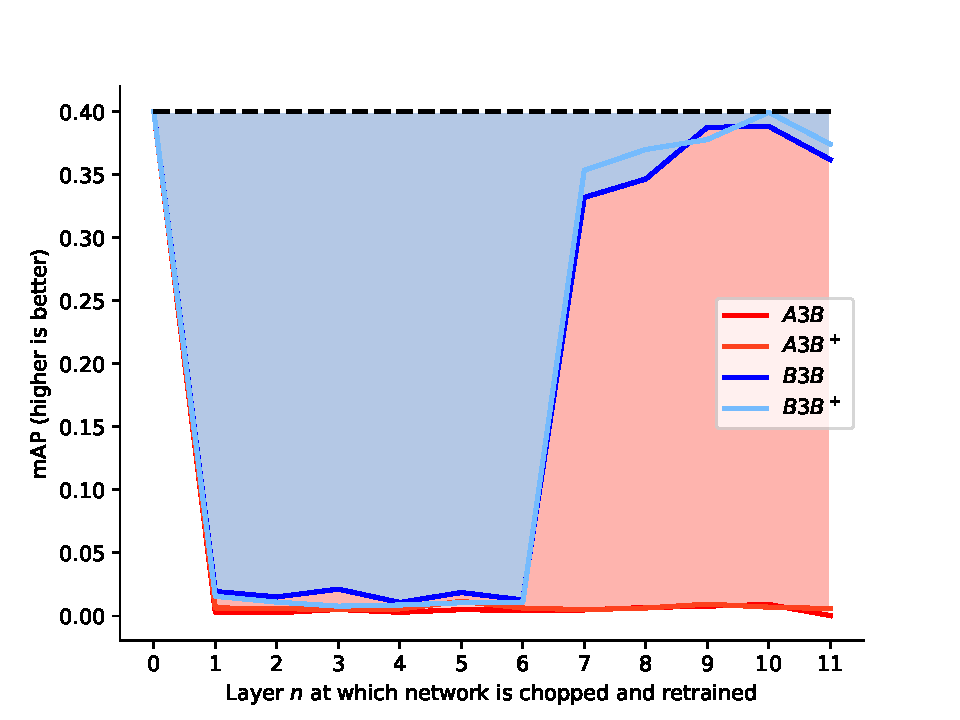
\includegraphics[width=\textwidth]{figures/experiments/grantExp.pdf}
\caption[Η μεταφερσιμότητα των παραμέτρων του SqueezeDet από το σύνολο Α στο σύνολο Β]{Η μεταφερσιμότητα των παραμέτρων του SqueezeDet από το σύνολο Α στο σύνολο Β. Η έντονη μπλε γραμμή είναι το mAP του δικτύου $BnB$, η λιγότερο έντονη του δικτύου $BnB^+$, η έντονα κόκκινη του δικτύου $AnB$ και η λιγότερο έντονη του $AnB^+$.}
\label{fig:grantExpRes}
\end{figure}

\begin{figure}
\centering
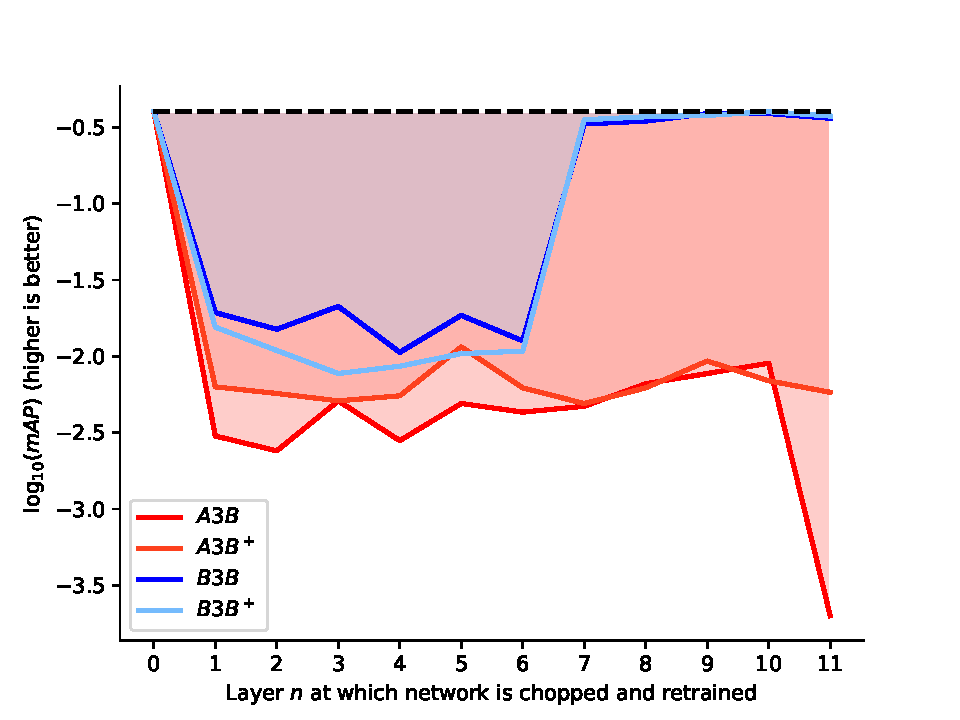
\includegraphics[width=\textwidth]{figures/experiments/grantExpLog.pdf}
\caption[Η μεταφερσιμότητα των παραμέτρων του SqueezeDet από το σύνολο Α στο σύνολο Β σε λογαριθμικό σκέλος]{Η μεταφερσιμότητα των παραμέτρων του SqueezeDet από το σύνολο Α στο σύνολο Β σε λογαριθμικό σκέλος. Η έντονη μπλε γραμμή είναι το mAP του δικτύου $BnB$, η λιγότερο έντονη του δικτύου $BnB^+$, η έντονα κόκκινη του δικτύου $AnB$ και η λιγότερο έντονη του $AnB^+$. Οι διαφορές μεταξύ των $BnB$ και $BnB^+$ διακρίνονται περισσότερο. }
\label{fig:grantExpResLog}
\end{figure}


\section{Αυτόματη επιλογή υπερπαραμέτρων}
\label{section:autohyperparamters}
Κατά την εκπαίδευση δεν υπάρχει βεβαιότητα ότι η επιλογή των υπερπαραμέτρων ήταν η βέλτιστη ή τουλάχιστον αρκετά κοντά σε αυτή. Για αυτό το σκοπό πέρα από την αναζήτηση με δοκιμές  και χρήση της διαίσθησης η οποία είναι αρκετές φορές λανθασμένη, χρησιμοποιήθηκε και μία άλλη μέθοδος βελτιστοποίησης των υπεραπαραμέτρων. Αυτή δεν απαιτεί τη χρήση παραγώγων (\textit{derivative free}) της συνάρτησης σφάλματος. Η μέθοδος αυτή αναφέρεται στο \cite{64} και πρόκειται για μέθοδο καθολικής βελτιστοποίησης.

Ο μόνος περιορισμός που λαμβάνει υπόψη αυτή η μέθοδος είναι ότι η συνάρτηση για την οποία γίνεται η αναζήτηση της βέλτιστης τιμής θα πρέπει να είναι τύπου \textit{Lipschitz}. Βεβαίως, αυτό είναι ήδη γνωστό για τα νευρωνικά δίκτυα ακόμα και αυτού του τύπου, αφού όλες οι συναρτήσεις που χρησιμοποιούνται είναι γραμμικές ή τμηματικά γραμμικές και όλοι οι μετασχηματισμοί αφορούν συνελίξεις με πεπερασμένα σήματα. Αυτό επιτρέπει την χρήση αυτής της μεθόδου. Οποιαδήποτε άλλη ιδιότητα και αν έχει το νευρωνικό ο αλγόριθμος βελτιστοποίησης των παραμέτρων το λαμβάνει υπόψη ως μαύρο κουτί.

Προκειμένου να εξερευνηθεί αν χρειάζεται η εφαρμογή κάποιου τέτοιου τύπου αλγορίθμου στο προηγούμενο πείραμα του κεφαλαίου επιλέχθηκε ένα σημείο του παραπάνω πειράματος, συγκεκριμένα στο σημείο ($AnB^+, n=10$) στο Σχήμα \ref{fig:grantExpRes} και διερευνήθηκε αν με τη χρήση του παραπάνω αλγορίθμου και με τις σωστές υπερπαραμέτρους μπορεί να επιτευχθεί κάποιο καλύτερο αποτέλεσμα. O χώρος διερεύνησης των υπερπαραμέτρων δίνεται στον Πίνακα \ref{table:hypSearch}.

Το αποτέλεσμα της αναζήτησης μετά από $16$ βήματα ήταν η βέλτιστη τιμή $mAP=2\%$ (η αρχική ήταν $1.3\%$), για τιμές των υπερπαραμέτρων που παρουσιάζονται στον Πίνακα \ref{table:hypSearch}. Η τιμή αυτή δείχνει ότι δεν υπάρχει περιθώριο βελτίωσης ως προς αυτές τις υπερπαραμέτρους. Οπότε, δε χρειάζεται να επαναληφθεί το πείραμα της ενότητας \ref{section:TheExperiment} με διαφορετική τιμή αυτών των υπερπαραμέτρων.

% \begin{table}[]
% \centering
% \caption{Δοκιμαστικές εκπαιδεύσεις με χρήση μεθόδου βελτιστοποίησης των υπερπαραμέτρων}
% \label{table:hyperparams}
% \begin{tabular}{|l|l|}
% \hline
% \textbf{Αριθμός βημάτων} & \textbf{mAP} \\ \hline
% 0 & \\ \hline
% 1 & \\ \hline
% 2 & \\ \hline
% 3 & \\ \hline
% 4 & \\ \hline
% 5 & \\ \hline
% 6 & \\ \hline
% 7 & \\ \hline
% 8 & \\ \hline
% 9 & \\ \hline
% 10 & \\ \hline
% 11 & \\ \hline
% 12 & \\ \hline
% 13 & \\ \hline
% 14 & \\ \hline
% 15 & \\ \hline
% \end{tabular}
% \end{table}

\begin{table}[]
\centering
\caption{Ο χώρος αναζήτησης των βέλτιστων υπερπαραμέτρων και οι βελτιστοποιημένες τιμές τους μετά από $16$ βήματα}
\label{table:hypSearch}
\begin{tabular}{|l|l|l|l|}
\hline
\textbf{Όνομα υπερπαραμέτρου} & ελάχιστο & μέγιστο & βελτιστοποιημένη τιμή\\ \hline
\textit{MAX\_GRAD\_NORM} &  0.5 & 2.0 & 1.0\\ \hline
\textit{WEIGHT\_DECAY} &  0.00001 & 0.00100 & 0.0001\\ \hline
\textit{LEARNING\_RATE} & 0.01 &  0.10 & 0.02\\ \hline
\textit{LEAKY\_COEF} & 0.05 & 0.2 & 0.014\\ \hline
\textit{KEEP\_PROB} & 0.10 &  0.75 & 0.6\\ \hline
\textit{LR\_DECAY\_FACTOR} & 0.1 & 0.7 & 0.65\\ \hline
\end{tabular}
\end{table}


% TODO: σχολιασμός αποτελεσμάτων

Τέλος, για να δικαιολογηθεί περαιτέρω η χρήση τέτοιων μεθόδων, επισημαίνεται ότι με αυτές δίνεται η δυνατότητα στον ερευνητή να έχει μία εποπτεία των περιοχών στις οποίες οι υπερπαράμετροι κάνουν το μοντέλο να αποκτά πιο θεμιτή συμπεριφορά. Ταυτόχρονα, η αναζήτηση αυτή γίνεται πιο γρήγορα χωρίς κενά χρόνου στα οποία οι υπολογιστικοί πόροι μένουν ανεκμετάλλευτοι.




\section{Σύνοψη \& Συμπεράσματα}
Το πείραμα δεν κρίνεται επιτυχημένο ως προς τη μεταφερσιμότητα των παραμέτρων καθώς η χρήση παραμέτρων από την εκπαίδευση στο KITTI δεν είχε θετικό αποτέλεσμα στην εκπαίδευση στο σύνολο δεδομένων B (παράγραφος \ref{subsection:Btrain}) του PASCAL\_VOC. Πιθανή αιτία αυτού είναι ο χαμηλός αριθμός δειγμάτων του συνόλου δεδομένων. Ωστόσο, ήταν δυνατή η παρουσίαση της ευθραυστότητας της συν-προσαρμογής των επιπέδων του SqueezeDet. Αυτή βρέθηκε να είναι αρκετά ισχυρή και μάλιστα να συνδέει τα $7$ πρώτα επίπεδα μεταξύ τους.

Αυτό δείχνει πως σε οποιαδήποτε μελλοντική μετεκπαίδευση του δικτύου SqueezeDet θα πρέπει να χρησιμοποιούνται υπερπαραμέτροι τουλάχιστον από τα $7$ πρώτα επίπεδα της προηγούμενης εκπαίδευσης. Ταυτόχρονα, και τα $7$ επίπεδα θα πρέπει να είναι εκπαιδεύσιμα, διαφορετικά δε θα γίνεται καλή γενίκευση στην μετεκπαίδευση του δικτύου.

Επίσης, έγινε αναζήτηση των βέλτιστων υπερπαραμέτρων με μέθοδο μη γραμμικής βελτιστοποίησης. Αυτή δεν παρήγαγε κάποιο αποτέλεσμα ικανά διαφορετικό, ώστε να χρειαστεί να επαναληφθεί το πείραμα με νέες υπερπαραμέτρους. Βέβαια, δεν εξετάστηκαν όλοι οι υπερπαραμέτροι όπως για παράδειγμα τα αρχικά μεγέθη των anchors που παράγει το δίκτυο. Ωστόσο, για αυτά έγιναν αρκετές δοκιμές πριν την εκπαίδευση στο σύνολο B και το τελικό πείραμα της ενότητας \ref{section:TheExperiment}. Επιπλέον, η αναζήτηση αυτών απαιτεί αρκετά περισσότερη υπολογιστική ισχύ από ότι μπορεί να προσφέρει η συστοιχία του εργαστηρίου, ώστε να γίνει σε λογικό χρονικό διάστημα, λόγω των πολλών διαστάσεων του προβλήματος βελτιστοποίησης.

Η εκτέλεση του πειράματος σε άλλα σύνολα δεδομένων αφήνεται ως μελλοντική εργασία, ώστε να δειχθεί αν το πείραμα μπορεί να είναι πετυχημένο πλήρως σε κάποιο άλλο σύνολο δεδομένων. Η εύρεση του ωστόσο είναι δύσκολη καθότι θα πρέπει να ληφθούν υπόψη οι περιορισμοί που θέτει το SqueezeDet προκειμένου να διατηρηθεί η μικρή μνήμη και η ταχύτητα που το χαρακτηρίζουν. % writting
\chapter{Επιτάχυνση του δικτύου SqueezeDet}
\label{chapter:accel_SqueezeDet}
Όπως έχει ήδη αναφερθεί, το συνολικό πείραμα για τη μελέτη της μεταφερσιμότητας των παραμέτρων απαιτεί αρκετό χρόνο σε ημέρες. Επιπλέον, ο υπολογιστικός φόρτος που επιβάλλει το πείραμα αυτό είναι θεμιτό να είναι ικανοποιητικά μικρός, ώστε και άλλοι χρήστες να μπορούν να εργαστούν στην υπολογιστική συστοιχία του εργαστηρίου. Επίσης, είναι αναγκαία η οποιαδήποτε επιτάχυνση του δικτύου προκειμένου να επιταχυνθεί το πείραμα. Η μεθοδολογία μίας τέτοιας επιτάχυνσης θα μπορούσε μελλοντικά να εφαρμοστεί και σε άλλες εκπαιδεύσεις δικτύων.

\section{Προβλήματα της αρχικής υλοποίησης}
\label{section:oldProblems}
Η αρχική υλοποίηση του SqueezeDet βρίσκεται δημοσιευμένη στο github \footnote{\url{https://github.com/BichenWuUCB/squeezeDet}}. Μετά από μελέτη της υλοποίησης αυτής γίνεται κατανοητό πως συνεχώς γίνονται μεταφορές δεδομένων από τη μνήμη του επεξεργαστή στη μνήμη της GPU και ότι οι περισσότερες μεταφορές δεδομένων είναι άσκοπες. Επίσης, απαιτείται αρκετή υπολογιστικής ισχύς από πλευράς της CPU, και η απαίτηση αυτή προκαλεί καθυστέρηση της εκπαίδευσης. Πιο αναλυτικά, τα προβλήματα που αναφέρονται στη λίστα παρακάτω είναι κατά σειρά σύμφωνα με τη ροή μετάδοσης πληροφορίας:

\begin{figure}
\centering
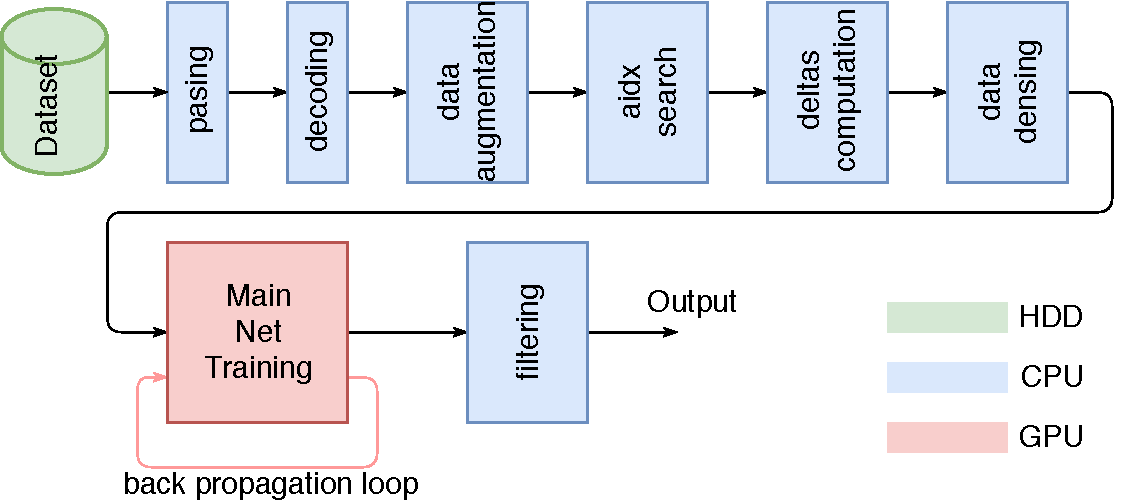
\includegraphics[width = \textwidth]{figures/experiments/old_pipeline.pdf}
\caption[Η σειρά ροής πληροφορίας στην αρχική υλοποίηση της εκπαίδευσης]{Η σειρά ροής πληροφορίας στην αρχική υλοποίηση της εκπαίδευσης. Όπως φαίνεται όλα τα επίπεδα που επεξεργάζονται τα δεδομένα εισόδου βρίσκονται στη μεριά της CPU. Μόνο τα επίπεδα του δικτύου (χωρίς το τελικό φίλτρο) βρίσκονται στην GPU, δηλαδή το εμπρόσθιο και το προς τα πίσω πέρασμα κατά την εκπαίδευση με back-propagation (περισσότερες πληροφορίες για το back-propagation στο \cite{66}). Η προ-επεξεργασία των εισόδων γίνεται σε πολλαπλά νήματα (8) που το κάθε ένα νήμα αναλαμβάνει μία εικόνα.}
\label{fig:old_pipeline}
\end{figure}




\begin{enumerate}
\label{enumerate:net_problems}
\item{Η ανάγνωση και η ανάλυση (parsing) των δεδομένων γίνονται χρησιμοποιώντας τη ανεπεξέργαστη μορφή τους όπως αυτή δίνεται από το αρχικό σύνολο δεδομένων, απαιτώντας τη δέσμευση αρκετής μνήμης για τη φόρτωση όλων των ετικετών του συνόλου δεδομένων στη μνήμη, ενώ ταυτόχρονα για οποιαδήποτε επιπλέον δεδομένα όπως οι εικόνες, η εξόρυξη τους εξαρτάται από το εκάστοτε σύστημα αρχείων. Επίσης, η ανάγνωση και η ανάλυση των δεδομένων βασίζονται σε βιβλιοθήκες υλοποίησης νηματικού προγραμματισμού στην python.}
\item{Η μεταφορά των πινάκων (και των τανυστών) στη GPU γίνεται χρησιμοποιώντας την πυκνή αναπαράσταση πινάκων, ενώ η φύση του προβλήματος επιτρέπει τη μεταφορά πινάκων υπό αραιή αναπαράσταση.}
\item{Οι εικόνες αποκωδικοποιούνται στην πλευρά της CPU και μετά αποστέλλονται στη GPU ως πίνακες με αναπαράσταση αριθμού κινητής υποδιαστολής, πράγμα που πέραν της παραπάνω απαίτησης μνήμης για τη μεταφορά, απαιτεί τη χρήση της εξωτερικής βιβλιοθήκης openCV \footnote{\url{https://opencv.org}} και επιβαρύνει την CPU με μία εργασία η οποία μπορεί να γίνει και στην GPU.}
\item{Το επόμενο βήμα μετά την αποκωδικοποίηση της εικόνας στην CPU είναι η ενίσχυση των δεδομένων (\textit{data augmentation}) στις εικόνες από τη CPU. Αυτή είναι μία αρκετά δαπανηρή υπολογιστικά διαδικασία για τη CPU από ότι για την GPU καθώς απαιτεί κυρίως μεταφορές δεδομένων οι οποίες είναι πλήρως παραλληλοποιήσιμες. Αυτή η διαδικασία μαζί με την παρακάτω κάνουν εκτενή χρήση της βιβλιοθήκης numpy και openCV.}
\item{Η διαδικασία αντιστοίχησης των anchors γίνεται επίσης από πλευράς CPU. Αυτό από μόνο του δεν έχει κάποιο συμφέρον να παραλληλοποιηθεί στη GPU, καθώς κάθε αποτέλεσμα αντιστοίχησης του αλγορίθμου εξαρτάται πλήρως από όλα τα προηγούμενα, ωστόσο απαιτεί τα προηγούμενα στάδια να βρίσκονται στη CPU.}
\item{Ο υπολογισμός των επιθυμητών deltas, ο οποίος είναι πλήρως παραληλλοποιήσιμος γίνεται στην CPU και μετά αποστέλλονται τα αποτελέσματα στην GPU. Αυτός θα μπορούσε να γίνεται απευθείας στην GPU από τη στιγμή που τα anchors είναι γνωστά από το προηγούμενο στάδιο.}
\item{Οι περισσότερες από τις πράξεις στην GPU όπως και στη CPU χρησιμοποιούν την πυκνή μορφή αραιών πινάκων απαιτώντας επεξεργαστικούς πυρήνες οι οποίοι κάνουν μη αναγκαίους υπολογισμούς του τύπου $ 0 \times 0 $ ή $ 0 \times a $, όπου $a$ στοιχείο πίνακα.}
\item{Το τελικό φίλτρο του δικτύου βρίσκεται υλοποιημένο στην CPU, γραμμένο σε python με χρήση της βιβλιοθήκης numpy. Αυτό απαιτεί πάλι μεταφορά αρκετά μεγάλων και πυκνών πινάκων (χωρίς δυνατότητα αραιής αναπαράστασης) από τη GPU στη CPU και τη μετέπειτα επεξεργασία τους.}
\item{Η επεξεργασία των αποτελεσμάτων για την οπτικοποίησή τους γίνεται με χρήση δύο βιβλιοθηκών του tensorflow και της openCV, ενώ μπορεί να γίνει απλά χρησιμοποιώντας μία στην πλευρά της GPU απαιτώντας μόνο τη μεταφορά λίγων δεδομένων από την GPU στη CPU πριν αποθηκευτούν στο σκληρό δίσκο.}
\end{enumerate}

Αυτά όλα είναι προβλήματα τα οποία επιλύθηκαν στα πλαίσια αυτής της διπλωματικής. Η επίλυσή τους και τα πλεονεκτήματα της μεθοδολογίας επίλυσης βρίσκονται σε αντιστοιχία με τη παραπάνω λίστα αυτής της ενότητας στη λίστα της ενότητας \ref{section:new_solutions}. Για την καλύτερη εικόνα των δύο υλοποιήσεων στο Σχήμα \ref{fig:old_pipeline} βρίσκεται η σειρά ροής πληροφορίας στην αρχική υλοποίηση, ενώ στο Σχήμα \ref{fig:new_pipeline} αναπαρίσταται η σειρά ροής πληροφορίας και τα στάδια της καινούριας υλοποίησης.

\section{Οι λύσεις της καινούριας υλοποίησης}
\label{section:new_solutions}
Η καινούρια υλοποίηση επέφερε αλλαγές στα στάδια ροής της πληροφορίας, λύνοντας τα προβλήματα που αναφέρθηκαν στην ενότητα \ref{section:oldProblems}. Οι λύσεις αυτές και το σκεπτικό της μεθοδολογίας αναλύονται στην παρακάτω λίστα. Όσα περιγράφονται παρακάτω δε σημαίνει ότι λύνουν πλήρως το πρόβλημα της επιτάχυνσης της εκπαίδευσης του δικτύου. Μία τεράστια επιτάχυνση θα ήταν εφικτή αν τοποθετούσαμε τα σύνολα δεδομένων σε σκληρό δίσκο SSD. Ωστόσο, αυτή μπορεί να συμβεί μόνο στην καινούρια υλοποίηση όπου δεν τίθεται όριο απόδοσης από τη CPU όπως πριν.

\begin{enumerate}
\label{enumerate:net_solutions}
\item{Σε αντίθεση με την αρχική υλοποίηση, η ανάγνωση και η ανάλυση (\textit{parsing}) των δεδομένων γίνεται σε αρχεία ειδικά διαμορφωμένα με χρήση των δομών \textit{protocol buffers} που παρέχει η βιβλιοθήκη Tensorflow. Κατά αυτό τον τρόπο η ανάγνωσή τους γίνεται με βάση τις προτάσεις της ομάδας ανάπτυξης της βιβλιοθήκης προς τη βελτιστοποίηση της απόδοσης μεταφοράς δεδομένων \footnote{\url{https://www.tensorflow.org/performance/datasets_performance}}. Πιο συγκεκριμένα χρησιμοποιείται προ-μεταφορά των δεδομένων (\textit{prefetching}) πριν την αποστολή τους στη GPU, ενώ ταυτόχρονα η τυχαία ανάμιξη αυτών γίνεται σε προκαθορισμένο χώρο μνήμης. Αυτά όλα έχουν ως αποτέλεσμα και την ανεξαρτησία από το σύστημα αρχείων, καθότι γίνεται ανάγνωση ενός μόνο αρχείου. Ταυτόχρονα, γίνεται χρήση προκαθορισμένου ποσού μνήμης ανεξαρτήτως από το σύνολο δεδομένων, το οποίο καθιστά την εκτέλεση της εκπαίδευσης πιο ασφαλή. Όλα αυτά γίνονται χωρίς την χρήση επιπλέον συναρτήσεων βιβλιοθηκών υλοποίησης νηματικού προγραμματισμού πέρα από τις συναρτήσεις του Tensorflow.}
\item{Πλέον, απαιτείται η μεταφορά μόνο των πινάκων με δεδομένα ετικετοποίησης (ξεχωριστά από την εικόνα) όπως οι συντεταγμένες των ορθογώνιων περιβλημάτων αντικειμένων και η κλάση κάθε αντικειμένου. Επίσης, όλοι οι πίνακες μεταφέρονται σε αραιή μορφή, επιτρέποντας τη μαζική μεταφορά πινάκων στη GPU πιο γρήγορα και χωρίς άσκοπα δεδομένα.}
\item{Η αποκωδικοποίηση των εικόνων δεν είναι εφικτό να γίνει στην πλευρά της GPU. Παρόλα αυτά προς αυτό το σκοπό χρησιμοποιήθηκε μόνο η βιβλιοθήκη του tensorflow, αναιρώντας την απαίτηση για χρήση της βιβλιοθήκης openCV ή της numpy. Ταυτόχρονα, η μεγέθυνση ή η σμίκρυνση της εικόνας γίνεται στην πλευρά της GPU.}
\item{Η ενίσχυση των δεδομένων (\textit{data augmentation}) γίνεται πλέον στην πλευρά της GPU λαμβάνοντας υπόψη ότι αυτή είναι μία πλήρως παραλληλοποιήσιμη διαδικασία. Σε αυτό το σημείο εξοικονομείται αρκετή επεξεργαστική ισχύς στη CPU, ενώ πάλι δεν χρειάζεται η χρήση επιπλέον βιβλιοθηκών.}
\item{Η διαδικασία αντιστοίχησης των anchors γίνεται μέσα στη GPU, ώστε να είναι εφικτά αυτά που αναφέρονται στα δύο σημεία παραπάνω. Η ανάλυση της παραλληλοποίησης αυτής της διαδικασίας είναι αρκετά αξιοσημείωτη και παρατίθεται στην παράγραφο \ref{subsection:par_anchor_alg}.}
\item{Ο υπολογισμός των επιθυμητών deltas, ο οποίος είναι πλήρως παραληλλοποιήσιμος γίνεται πλέον από την GPU και μάλιστα με χρήση αραιών πινάκων, δίνοντας μία επιπλέον επιτάχυνση στην εκπαίδευση.}
\item{Οι περισσότερες πράξεις στη GPU γίνονται πλέον με χρήση αραιών πινάκων, ενώ προτιμάται η επιλογή τιμών από πυκνούς πίνακες από ότι η μετατροπή αραιών σε πυκνούς όπου αυτό είναι εφικτό για τη μείωση των πυρήνων της GPU που χρησιμοποιούνται στους υπολογισμούς τόσο του εμπρόσθιου περάσματος του δικτύου όσο και του οπίσθιου (έχοντας κατά νου τον αλγόριθμο back-propagation). Κατά αυτό τον τρόπο μειώνεται αρκετά και το ποσοστό χρήσης της GPU, χωρίς απαραίτητα να μειώνονται οι χρόνοι υπολογισμού.}
\item{Το τελικό φίλτρο του δικτύου είναι υλοποιημένο στην GPU και γραμμένο χρησιμοποιώντας τη βιβλιοθήκη Tensorflow. Αυτό πρώτον ελαφρύνει τη μεταφορά των δεδομένων γιατί πλέον δεν χρειάζεται η μεταφορά πυκνών πινάκων από τη GPU στη CPU και μπορεί κανείς να λάβει απευθείας το τελικό αποτέλεσμα. Δεύτερον, μετά την εκπαίδευση ή την μετεκπαίδευση είναι δυνατή η εξαγωγή του γράφου και η χρήση του σε οποιοδήποτε σύστημα/γλώσσα που υποστηρίζει το Tensorflow ακόμα και ενσωματωμένου (με χρήση του \textit{Tensorflow lite}\footnote{\url{https://www.tensorflow.org/mobile/tflite/}}) ως “μαύρο κουτί” χωρίς τη συγγραφή επιπλέον κώδικα ο οποίος απαιτεί την γνώση των τελικών διαστάσεων του δικτύου και γενικότερα εννοιών που αφορούν εσωτερικά το δίκτυο.}
\item{Η επεξεργασία των αποτελεσμάτων πριν την οπτικοποίησή τους επίσης γίνεται στη GPU, με χρήση μόνο του Tensorflow και αποστολή μόνο των απαραιτήτων δεδομένων στην CPU και στο σύστημα αρχείων.}
\end{enumerate}

\begin{figure}
\centering
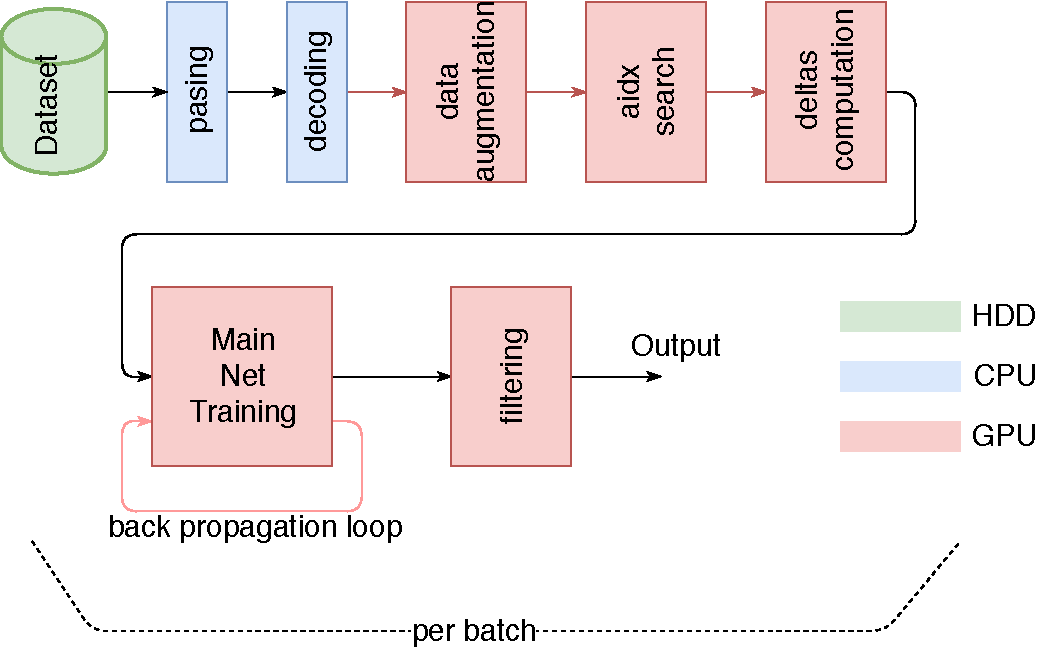
\includegraphics[width = \textwidth]{figures/experiments/new_pipeline.pdf}
\caption[Η σειρά ροής πληροφορίας στην καινούρια υλοποίηση της εκπαίδευσης]{Η σειρά ροής πληροφορίας στην καινούρια υλοποίηση της εκπαίδευσης. Η ανάγνωση του συνόλου δεδομένων μαζί με την αποκωδικοποίηση εικόνας είναι τα μοναδικά επίπεδα του δικτύου τα οποία βρίσκονται από τη μεριά της CPU και πραγματοποιούνται από πληθώρα νημάτων (8). Τα υπόλοιπα επίπεδα βρίσκονται στην GPU και μόνο η τελική έξοδος, μετά το τελικό φίλτρο, όταν χρειασθεί μεταφέρεται στην μεριά της CPU. Επίσης, η συνολική τροφοδοσία και επεξεργασία των δεδομένων γίνεται σε συστάδες.}
\label{fig:new_pipeline}
\end{figure}

\section{Παραλληλοποίηση διαδικασίας αντιστοίχησης των anchors}
\label{subsection:par_anchor_alg}

Η παραλληλοποίηση αυτού του αλγορίθμου είναι αρκετά σημαντική, διότι αυτή είναι που ουσιαστικά επιτρέπει την υλοποίηση της πλήρης εκπαίδευσης του δικτύου στη GPU. Ωστόσο, δεν περιορίζεται σε αυτό το δίκτυο μόνο, αλλά μπορεί να χρησιμοποιηθεί σε όλα τα δίκτυα εντοπισμού αντικειμένων τα οποία βασίζονται σε anchors. Επίσης, η υλοποίηση του αλγορίθμου \ref{alg:Tensor} είναι ελαχιστοποιημένη ώστε να μπορέσει να προστεθεί ως κόμβος στον ευρύτερο υπολογιστικό γράφο εκπαίδευσης του δικτύου. Έτσι λοιπόν υπάρχει η δυνατότητα επαναχρησιμοποίησης του αλγορίθμου στην εκπαίδευση οποιουδήποτε άλλου νευρωνικού δικτύου το οποίο χρησιμοποιεί anchors. Αντίθετα, ο μόνος αντίστοιχος αλγόριθμος που βρέθηκε \footnote{\url{https://github.com/nilboy/tensorflow-yolo/tree/python2.7/yolo/net}} αφορά συγκεκριμένα μόνο το YOLO, δεν έχει την ευελιξία χρησιμοποίησης σε άλλα νευρωνικά δίκτυα και είναι υπολογιστικά πιο δαπανηρός, αφού η σειριακή επανάληψη που εμπεριέχει απαιτεί περισσότερο χρόνο σε κάθε βήμα.

Στο πρώτο κομμάτι της ανάλυσης παρουσιάζεται ο σειριακός αλγόριθμος, ο οποίος βρίσκεται στην αρχική υλοποίηση γραμμένος σε python. Παρόλα αυτά, εδώ \ref{alg:serial} παρουσιάζεται σε μορφή ψευδοκώδικα. Στον αλγόριθμο \ref{alg:parallel} παρουσιάζεται η παράλληλη μορφή που μπορεί να εκτελεστεί στη GPU ή σε οποιαδήποτε άλλη πλατφόρμα που υποστηρίζει παράλληλη εκτέλεση αλγορίθμων. Για την υλοποίηση ωστόσο με χρήση της βιβλιοθήκης του Tensorflow ο αλγόριθμος \ref{alg:serial} θα χρειαστεί να γραφεί με χρήση πινάκων και γραμμικής άλγεβρας. Προφανώς η άμεση υλοποίηση σε κάποια βιβλιοθήκη όπως η CUDA \footnote{\url{https://developer.nvidia.com/cuda-zone}} μπορεί να δώσει πιο γρήγορα αποτελέσματα από ότι το Tensorflow. Η υλοποίηση σε CUDA και συμπερίληψη αυτού του κομματιού στο Tensorflow αφήνεται ως μελλοντική εργασία.

\begin{algorithm}
\caption{
 Στην είσοδο του σειριακού αλγορίθμου η είσοδος $ ANCHOR\_BOX$ εμπεριέχει τα κουτιά των anchors μεγέθους $[ANCHORS, 4]$ όπου η σταθερά $ANCHORS$ είναι το πλήθος των ορθογωνίων κουτιών που προτείνει το νευρωνικό σε κάθε εμπρόσθιο πέρασμα χωρίς κάποιο φίλτρο. Η είσοδος $rois$ είναι μία λίστα από λίστες κουτιών από τα δεδομένα ετικετοποίησης. Πρόκειται για τα κουτιά που το νευρωνικό είναι θεμιτό να εντοπίζει. Η λίστα έχει μέγεθος $BATCH\_SIZE$ και κάθε μέλος της είναι από μόνο του μία λίστα κουτιών. Η είσοδος $BATCH\_SIZE$ είναι το μέγεθος το δειγμάτων (εικόνες) τα οποία χρησιμοποιούνται σε κάθε επανάληψη της εκπαίδευσης. Για να γίνει κατανοητό πως μπορεί να γίνει η αναπαράσταση ενός κουτιού παρατίθεται το Σχήμα \ref{fig:bboxPresentation}. Η συνάρτηση $len(\cdot)$ επιστρέφει το μήκος της πρώτης διάστασης της λίστας ή του πίνακα εισόδου και η συνάρτηση $d(\cdot,\cdot)$ είναι η συνάρτηση της ευκλείδειας απόστασης μεταξύ δύο διανυσμάτων. Η συνάρτηση $argsort(\cdot,\cdot)$ επιστρέφει τους δείκτες της μετάθεσης που πρέπει να γίνει ώστε να ταξινομηθεί ο πίνακας του πρώτου ορίσματος με αύξουσα ή φθίνουσα σειρά σύμφωνα με το δεύτερο όρισμα. Επίσης, όλα τα σύνολα που αναφέρθηκαν ή αναφέρονται παρακάτω είναι διακριτά με απόσταση στοιχείων 1, εκτός από το $aidx\_set$ που τα στοιχεία του ορίζονται ένα προς ένα στον αλγόριθμο. Οι κενές λίστες δηλώνονται ως $[]$ και τα κενά σύνολα ως $\{\}$, η πράξη πρόσθεσης στοιχείου είναι αντίστοιχα $\vee$ και $\cup$. }
\label{alg:serial}
\begin{algorithmic}
\Require ANCHOR\_BOX, rois, BATCH\_SIZE, ANCHORS
\For{$idx \in [0,\hdots,BATCH\_SIZE)$}
    \State $ gt\_bbox\gets rois[idx]$
    \State $aidx\_per\_image\gets []$
    \State $aidx\_set\gets \{\}$
    \For{$i \in [0,\hdots, len(gt\_bbox))$}
        \State $overlaps\gets IOU(b, gt\_bbox[i]), \forall b \in ANCHOR\_BOX$
        \State $aidx\gets ANCHORS$
        \For{$ov\_idx \in argsort(overlaps, "descending")$}
            \If{$overlaps[ov\_idx] \leq 0$}
                \State break
            \EndIf
            \If{$ov\_idx \notin aidx\_set$}
                \State $aidx\_set\gets aidx\_set \cup ov\_idx$
                \State $aidx\gets ov\_idx$
                \State break
            \EndIf
        \EndFor
        \If{$aidx = ANCHORS$}
            \State $dist = [d(gt\_bbox[i][:] - b[:]) \, \forall b \in ANCHOR\_BOX]$
            \For{$dist\_idx \in argsort(dist, "ascending")$}
                \If{$dist\_idx \notin aidx\_set$}
                    \State $aidx\_set\gets aidx\_set \cup dist\_idx$
                    \State $aidx\gets dist\_idx$
                    \State break
                \EndIf
            \EndFor
        \EndIf
        \State $aidx\_per\_image\gets aidx\_per\_image \vee aidx$
    \EndFor
    \State $aidx\_per\_batch\gets aidx\_per\_batch \vee aidx\_per\_image$
\EndFor\\
\Return $aidx\_per\_batch$
\end{algorithmic}
\end{algorithm}
Στη σειριακή υλοποίηση \ref{alg:serial} γίνεται εμφανές το κέρδος από την χρήση CPU στην εκτέλεση αυτού του αλγορίθμου από μόνο του. Ωστόσο, δε γίνονται εμφανείς οι απώλειες επίδοσης στα υπόλοιπα κομμάτια της υλοποίησης.


\begin{algorithm}
\caption{Η διαφορά στις εισόδους από τον σειριακό είναι ότι η είσοδος $rois$ είναι ένας πίνακας σε αραιή αναπαράσταση που έχει ως δείκτες τα στοιχεία $rois\_idx$ και ως τιμές τα στοιχεία $rois\_values$. Η συνάρτηση $dynamic\_partition(\cdot,\cdot)$ χωρίζει την πρώτη διάσταση του πίνακα σύμφωνα με τους δείκτες του δεύτερου ορίσματος σε υποπίνακες όπως φαίνεται στο Σχήμα \ref{fig:dynamicPartition}. Η συνάρτηση $shape(\cdot)$ επιστρέφει τις διαστάσεις του πίνακα ως μία λίστα. Η συνάρτηση $find\_best\_aidx\_per\_image$ είναι αυτή που επιλέγει τα aidx (δείκτες των anchors) για κάθε εικόνα. Η λειτουργία της είναι να λαμβάνει το πιο αριστερό στοιχείο διάφορο του $-1$ σε κάθε γραμμή του πίνακα $N$, ξεκινώντας από πάνω προς τα κάτω και κάθε φορά που επιλέγει ένα στοιχείο να τοποθετεί τη τιμή $-1$ σε όλα τα στοιχεία του πίνακα $N$ τα οποία έχουν την ίδια τιμή με το επιλεγόμενο στοιχείο.}
\label{alg:parallel}
\begin{algorithmic}
\Require ANCHOR\_BOX, rois, BATCH\_SIZE, ANCHORS
\State $S \gets [0,\hdots, len(rois\_values))$
\State $flat\_overlaps\gets IOU(b_1, b_2),\, \forall b_1 \in rois\_values, \forall b_2 \in ANCHOR\_BOX$
\State $max\_overlaps[i]\gets max(flat\_overlaps[i][:]) \forall i \in S$
\State $overlaps\_sorted\_idx[i]\gets argsort(flat\_overlaps[i][:], "descending"), \forall i \in S$
\State $flat\_dists\gets d(b_1,b_2), \forall b_1 \in rois\_values, \forall b_2 \in ANCHOR\_BOX$
\State $dists\_sorted\_idx\gets argsort(flat\_dists[i][:], "ascending"), \forall i \in S$
\For{$i \in S, j \in [0,\hdots,ANCHORS)$}
    \If{$max\_overlaps[i] \leq 0$}
        \State $all\_aidx[i][j]\gets dists\_sorted\_idx[i][j]$
    \Else
        \State $all\_aidx[i][j]\gets overlaps\_sorted\_idx[i][j]$
    \EndIf
\EndFor

\State $unstacked\_aidx\gets dynamic\_partition(all\_aidx, rois\_idx[:][0])$
\State $aidx\_values\gets \bigvee_{i=0}^{BATCH\_SIZE-1} find\_best\_aidx\_per\_image(unstacked\_aidx[i])$
\State $aidx\gets SparseArray(rois\_idx, aidx\_values)$\\
\Return $aidx$
\\
\Function{$find\_best\_aidx\_per\_image$}{$aidx\_slice$}
    \State $slice\_shape\gets shape(aidx\_slice)$
    \State $els\_used\gets [aidx\_slice[0][0], 0,\hdots,0]$
    % \State $neg\_ones\gets -\mathbf{1}_{i,j}, (i,j) \in \left[(0,0),\hdots,(shape(aidx\_slice)-(1,1))\right]$
    \State $N\gets aidx\_slice$
    \State $i\gets 1$
    \While{$i < len(aidx\_slice)$}
        \For{$j \in [0,\hdots,slice\_shape[1])$}
            \If{$N[i][j] = els\_used[i-1]$}
                \State $N[i][j]\gets -1$
            \EndIf
        \EndFor
        \State $s\gets \bigvee_{j=0}^{slice\_shape[1]-1} N[i][j] | N[i][j] \neq -1$
        \State $els\_used\gets s[0]$
        \State $i\gets i+1$
    \EndWhile\\
    \Return $els\_used$    
\EndFunction
\end{algorithmic}

\end{algorithm}
Στην παράλληλη υλοποίηση \ref{alg:parallel} φαίνεται ότι η συνάρτηση $find\_best\_aidx\_per\_image$ απαιτεί τον ίδιο χρόνο εκτέλεσης με τη σειριακή υλοποίησή της αν υποτεθεί ότι ο χρόνος εκτέλεσης του σώματος της επανάληψης $\mathbf{while}$ είναι σταθερός και της τάξης $O(1)$. Οπότε, στην καλύτερη περίπτωση το κομμάτι της συνάρτησης αυτής είναι ίσο με την σειριακή λύση του προβλήματος.


\begin{algorithm}
\caption{Το κυρίως μέρος σε αυτή τη μορφή του αλγορίθμου παραμένει ίδιο, το μόνο που διαφέρει είναι η συνάρτηση $find\_best\_aidx\_per\_image$. Σε αυτήν απαιτείται όλα τα βήματα μέσα στον βρόγχο επανάληψης $\mathbf{while}$ να υπολογίζονται ταυτόχρονα.}
\label{alg:Tensor}
\begin{algorithmic}
\Require ANCHOR\_BOX, rois, BATCH\_SIZE, ANCHORS\\
Main part is the same as the simple parallel algorithm.
\Function{$find\_best\_aidx\_per\_image$}{$aidx\_slice$}
    \State $slice\_shape\gets shape(aidx\_slice)$
    \State $els\_used\gets [aidx\_slice[0][0], 0,\hdots,0]$
    \State $neg\_ones\gets -\mathbf{1}_{i,j}, (i,j) \in \left[(0,0),\hdots,(shape(aidx\_slice)-(1,1))\right]$
    \State $N\gets aidx\_slice$
    \State $i\gets 1$
    \State $J\gets [0,\hdots,slice\_shape[1])$
    \While{$i < len(aidx\_slice)$}
        \State $N[i][j]\gets -1 \; \text{if}\; N[i][j] = els\_used[i-1] \; \text{else}\; N[i][j], j \in J$
        \State $els\_used\gets [els\_used[0],\hdots,els\_used[i-1],N[i,min(j|(N[i][j]\neq-1\, and \, N[i][j]\neq els\_used[i-1]))],0,\hdots,0] $
        \State $i\gets i+1$
    \EndWhile\\
    \Return $els\_used$    
\EndFunction

\end{algorithmic}

\end{algorithm}
Στην υλοποίηση με πράξεις πινάκων υπάρχει απώλεια επίδοσης, διότι δεν είναι δυνατή η εκμετάλλευση των ακραίων περιπτώσεων. Ως ακραίες περιπτώσεις λαμβάνονται οι περιπτώσεις κατά τις οποίες τα aidx βρίσκονται όλα στην πρώτη στήλη. Σε αυτή την περίπτωση ο παράλληλος αλγόριθμος όπως και ο τελευταία παρουσιαζόμενος αλγόριθμος \ref{alg:Tensor}, ο οποίος είναι ειδικά σχεδιασμένος για λειτουργία με τανυστές και πίνακες θα χρησιμοποιήσουν αρκετούς υπολογιστικούς πυρήνες της GPU για να δώσουν αποτέλεσμα σε χρόνο τουλάχιστον ίσο με τον σειριακό αλγόριθμο.

\begin{figure}
\centering
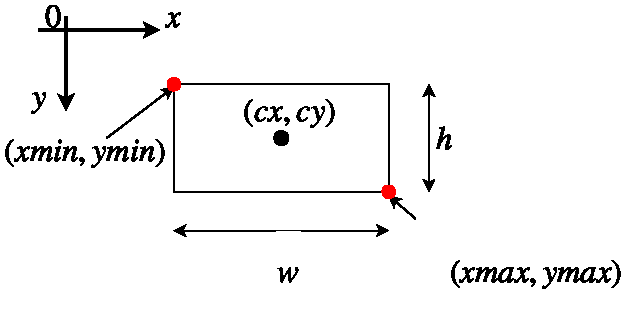
\includegraphics[width = 0.7\textwidth]{figures/experiments/bbox_presentation.pdf}
\caption[Αναπαράσταση ορθογωνίου περιοχής ενδιαφέροντος]{Οι περιοχές ενδιαφέροντος στις οποίες βρίσκονται αντικείμενα στις εικόνες και έχουν σχήμα ορθογώνιου κουτιού περιγράφονται από τέσσερις αριθμούς. Η πρώτη αναπαράσταση είναι με τους $(xmin,ymin,xmax,ymax)$ και η δεύτερη με τους $(cx,cy,w,h)$.}
\label{fig:bboxPresentation}
\end{figure}

\begin{figure}
\centering
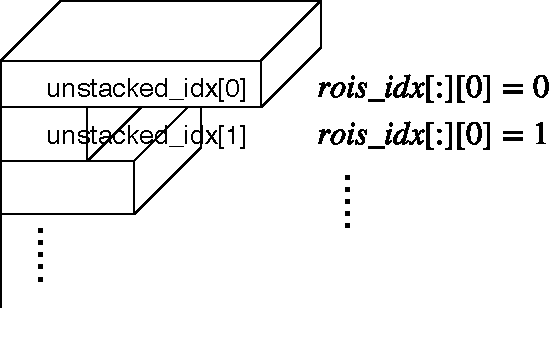
\includegraphics[width = 0.7\textwidth]{figures/experiments/dynamic_partition.pdf}
\caption[Δυναμικός κατακερματισμός πίνακα]{Το σχήμα περιγράφει τη λειτουργία της συνάρτησης $dynamic\_partition(all\_aidx, rois\_idx)$ που περιγράφεται στον αλγόριθμο \ref{alg:parallel}.} 
\label{fig:dynamicPartition}
\end{figure}


\section{Συνολική εικόνα των αλλαγών}
Συνολικά οι αλλαγές που έγιναν είναι η χρήση μόνο μίας εξωτερικής βιβλιοθήκης (Tensorflow) και η υλοποίηση όλου του δικτύου σε αυτή. Αυτό επιτρέπει τη χρήση του δικτύου ως “μαύρου κουτιού” από άλλα συστήματα. Ελαχιστοποίηση της μεταφοράς των δεδομένων και βελτιστοποίηση της επεξεργασίας τους μέσω της χρήσης αραιών πινάκων. Η μεταφορά όλων των υπολογισμών στην GPU, έκανε όχι μόνο πιο γρήγορο το δίκτυο όπως εξηγείται παρακάτω, αλλά μείωσε το φορτίο της CPU του συστήματος και της μνήμης δίνοντας τη δυνατότητα και στους άλλους χρήστες του συστήματος  να χρησιμοποιούν τη συστοιχία κατά το διάστημα των πειραμάτων μεταφερσιμότητας. Η μείωση αυτή του φορτίου παρουσιάζεται στο Σχήμα \ref{fig:loadCompare} και μπορεί να κάνει εφικτή την εκπαίδευση του δικτύου με χρήση επεξεργαστή χαμηλότερης απόδοσης.

Η καινούρια υλοποίηση ελέγχθηκε ως προς την ορθότητα στο σύνολο δεδομένων του KITTI \cite{80} σύμφωνα με τη μετρική mAP του συνόλου ελέγχου του KITTI. Σε αυτό βρέθηκε ότι πετυχαίνει επιτάχυνση του χρόνου εκπαίδευσης κατά $\sim1.8$ φορές σε σύγκριση με την αρχική υλοποίηση. Η σύγκριση των χρόνων εκπαίδευσης στο KITTI για τις πρώτες $20000$ επαναλήψεις φαίνεται στο Σχήμα \ref{fig:kittiCompare}. Επίσης, τα δεδομένα των χρόνων εκτέλεσης ανά κόμβο του υπολογιστικού γράφου παρουσιάζονται στο Σχήμα \ref{fig:kittiTracing}. Τονίζεται ότι μία εποχή στην εκπαίδευσή είναι $385$ επαναλήψεις. Οπότε, είναι αξιοσημείωτο ότι μία εποχή απαιτεί χρόνο ίσο με $\sim89 s$ στην καινούρια υλοποίηση ενώ στην παλαιότερη απαιτούσε χρόνο ίσο με $\sim160 s$. Τα αποτελέσματα (χρόνοι) για την καινούρια υλοποίηση στο PASCAL\_VOC φαίνονται στο Σχήμα \ref{fig:pascal_batches_per_sec}. Επιπλέον, για το ίδιο σύνολο δεδομένων τα δεδομένα των χρόνων εκτέλεσης ανά κόμβο του υπολογιστικού γράφου παρουσιάζονται στο Σχήμα \ref{fig:pascal_tracing}.


\begin{figure}
    \centering
    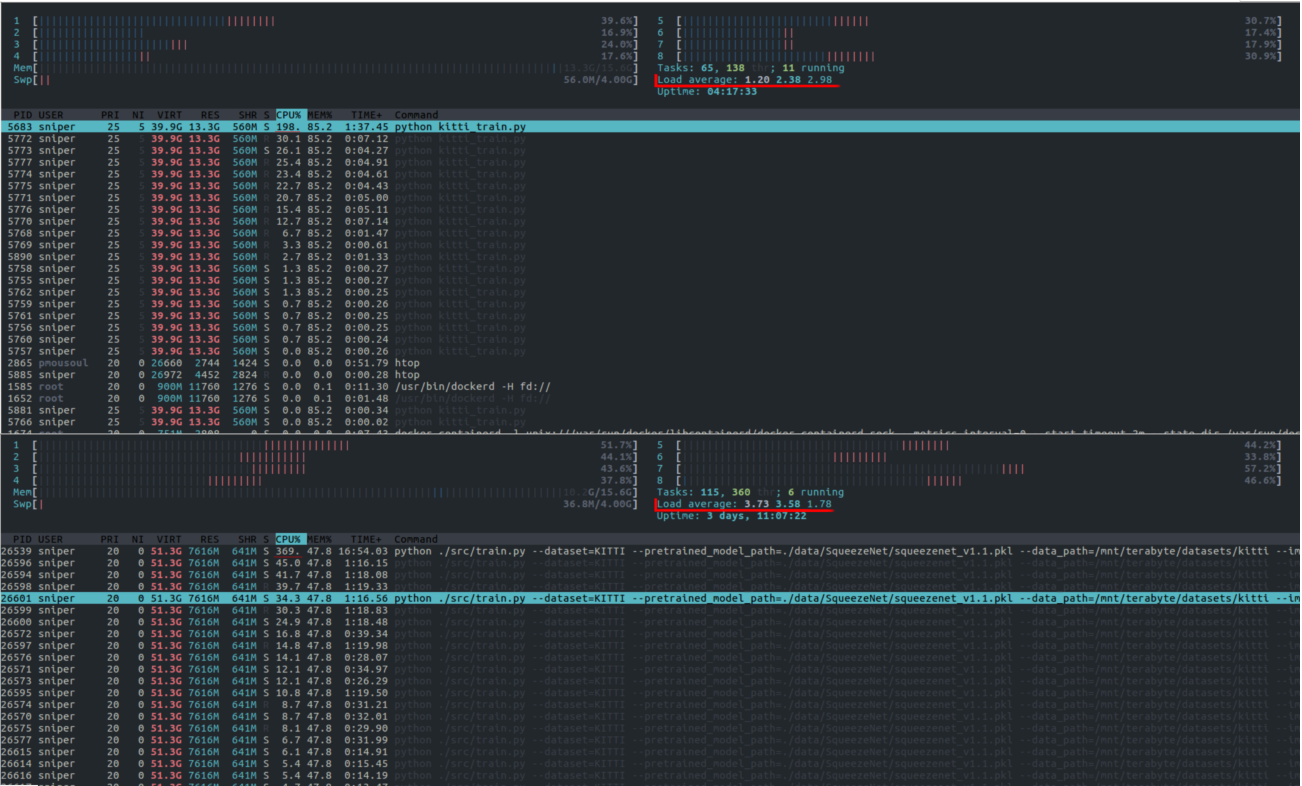
\includegraphics[width=\textwidth]{figures/experiments/load_comparison.pdf}
    \caption[Σύγκριση φορτίου υλοποιήσεων]{Το φορτίο του επεξεργαστή, της RAM και του συστήματος όπως παρουσιάζεται από την εντολή \textit{htop}\footnote{\url{https://hisham.hm/htop/}} κατά τη διάρκεια της εκπαίδευσης της καινούριας υλοποίησης πάνω και της παλιάς κάτω. Το φορτίο συστήματος της καινούριας ανέρχεται στη τιμή $1.2$ ενώ της παλιάς στη τιμή $3.73$.}
    \label{fig:loadCompare}
\end{figure}

\begin{figure}
    \centering
    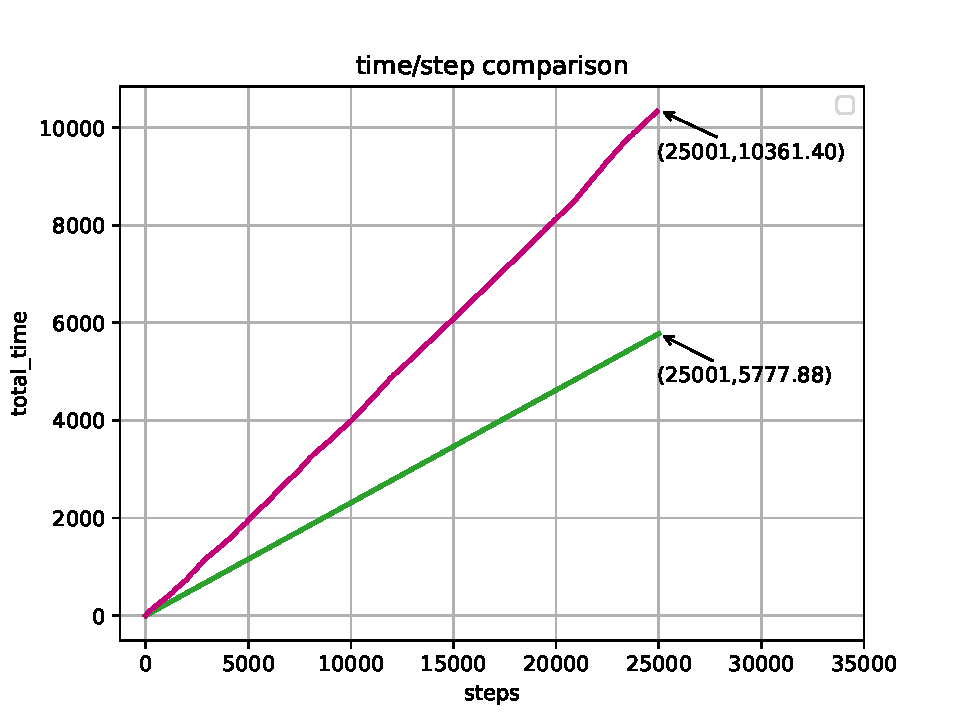
\includegraphics[width=\textwidth]{figures/experiments/kitti_compare.pdf}
    \caption[Σύγκριση χρόνων εκπαίδευσης στις δύο υλοποιήσεις]{Σύγκριση χρόνων εκπαίδευσης στις δύο υλοποιήσεις. Ο άξονας του χρόνου έχει μονάδα μέτρησης το δευτερόλεπτο. Η επιτάχυνση της καινούριας υλοποίησης έχει τιμή $1.799 \approx 1.8$. Με \textcolor{purple}{μωβ} διαγράφονται οι χρόνοι της παλιάς υλοποίησης και με \textcolor{SeaGreen}{πράσινο} της καινούριας.}
    \label{fig:kittiCompare}
\end{figure}


\begin{figure}
\centering
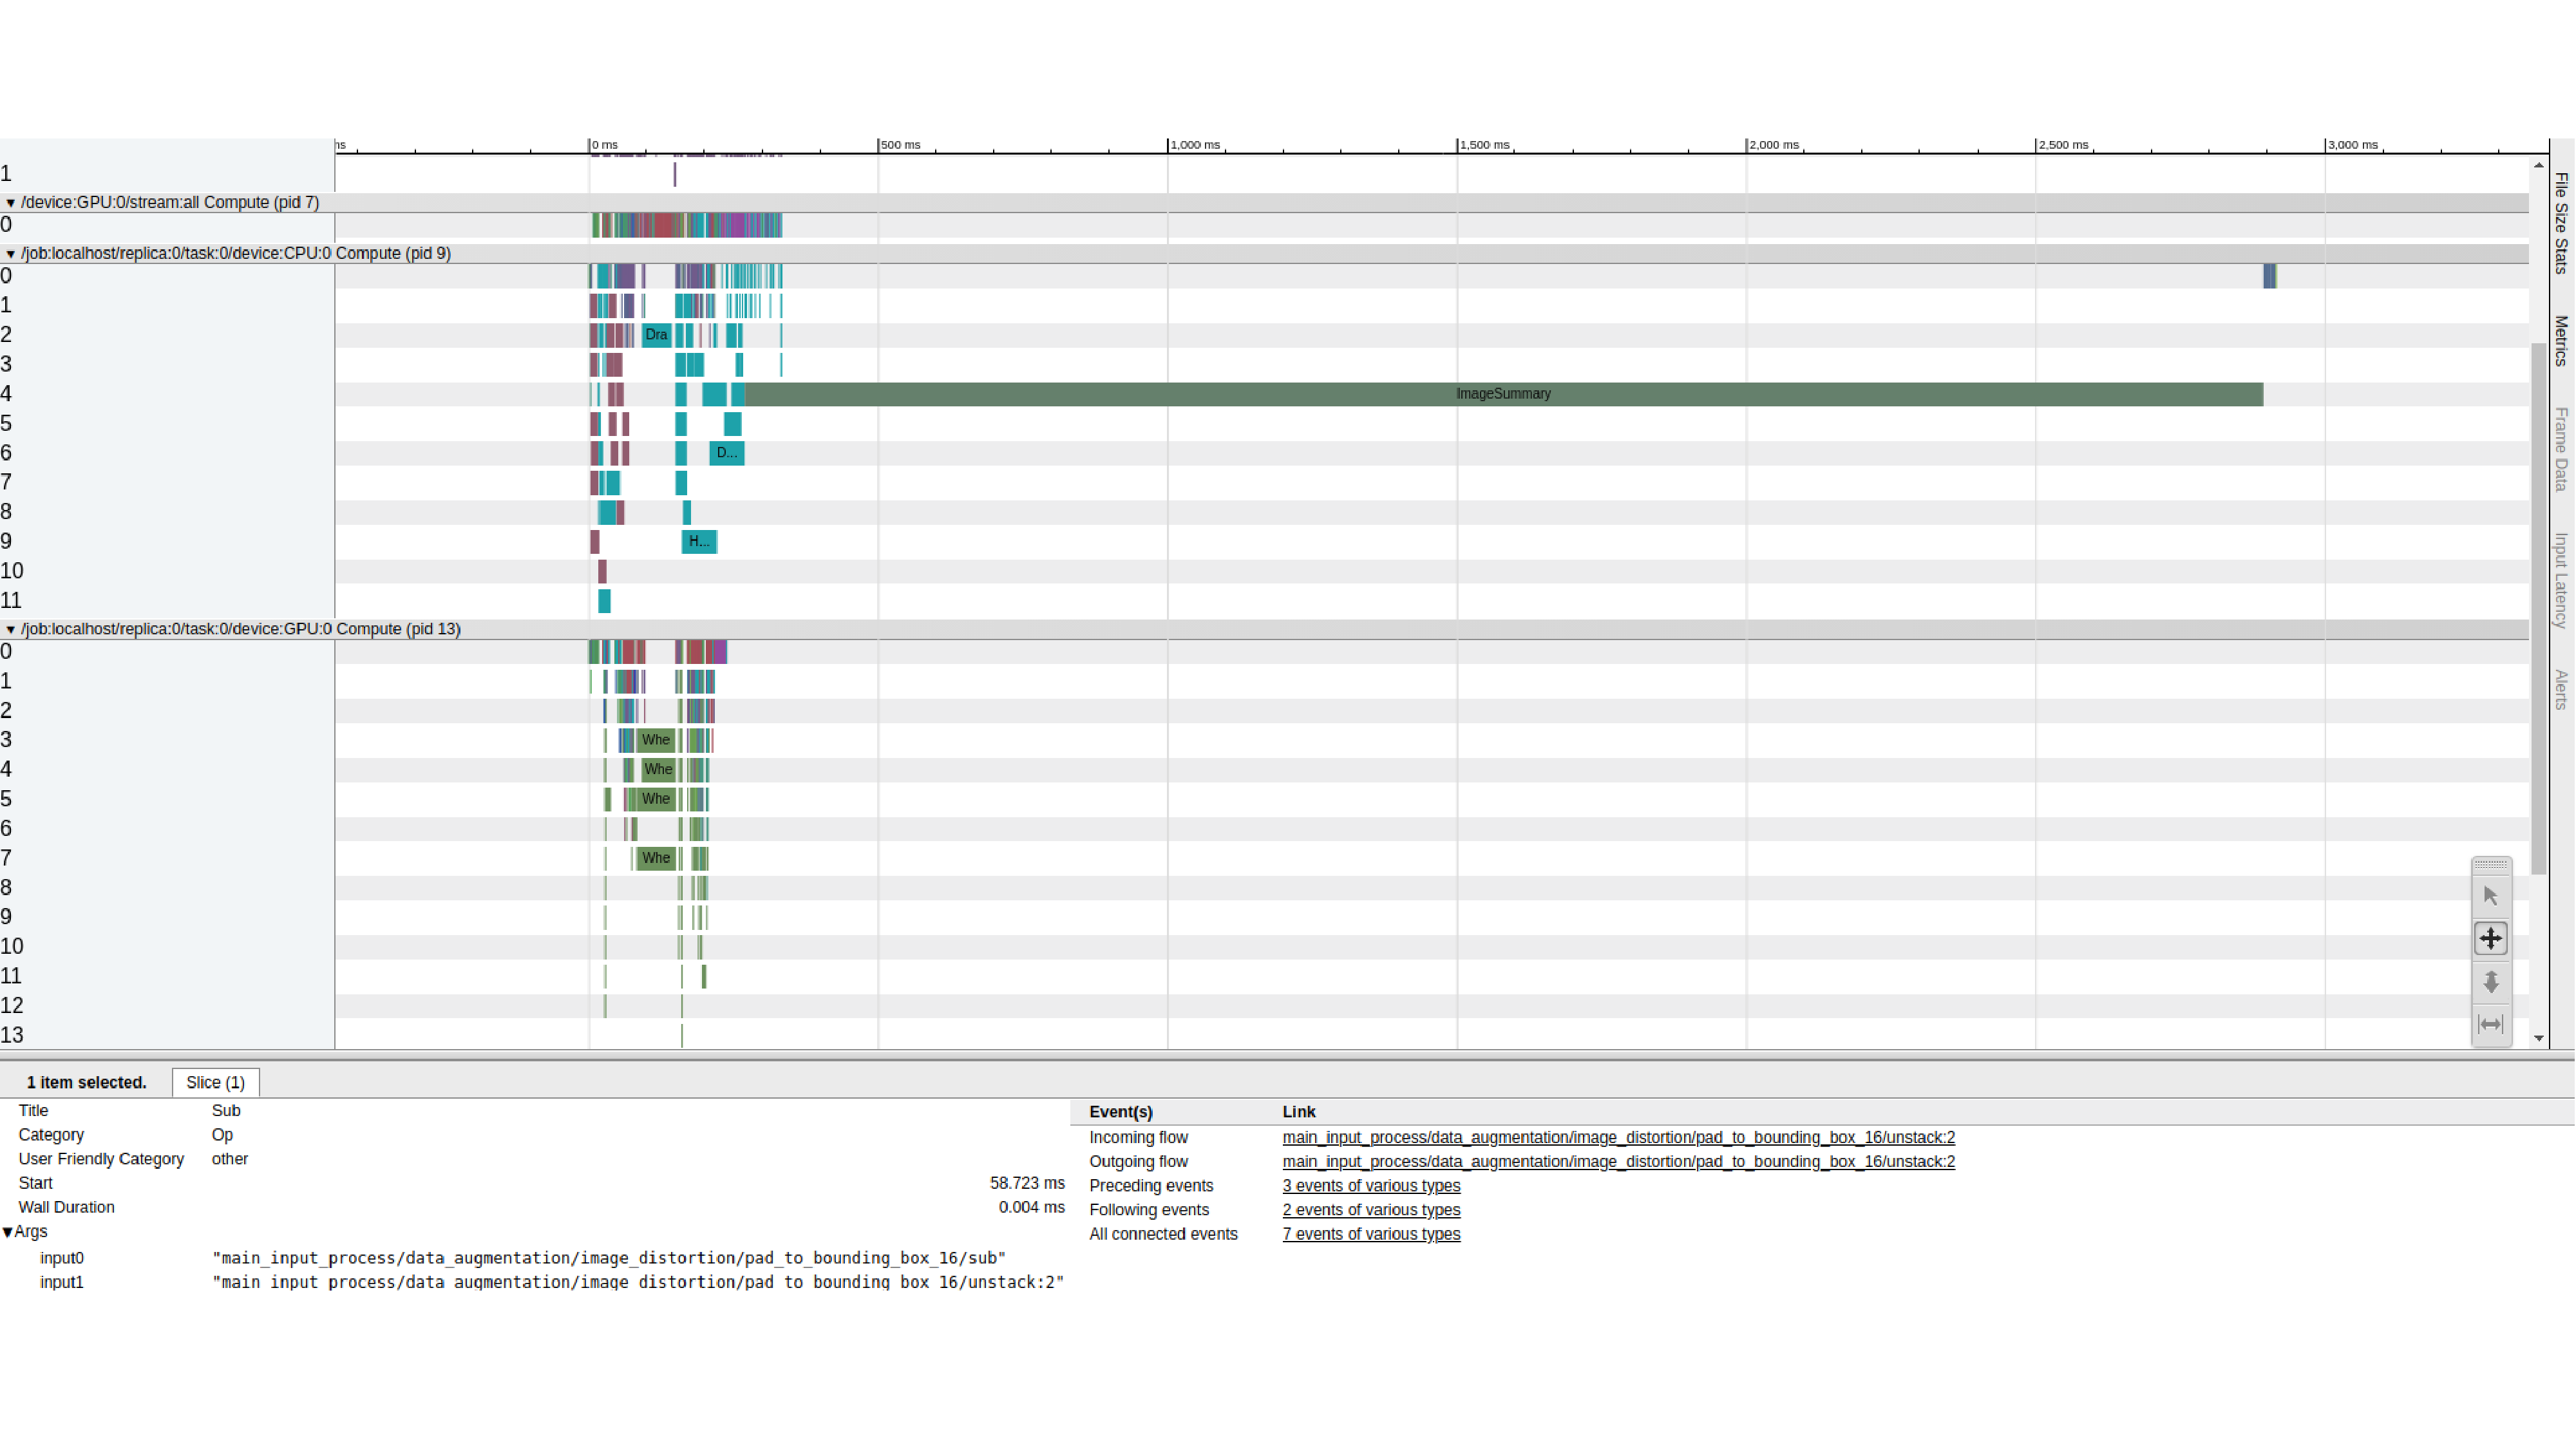
\includegraphics[width=\textwidth]{figures/experiments/kitti_new_tracing.pdf}
\caption[Χρόνοι εκτέλεσης κάθε επιπέδου στο KITTI]{Οι χρόνοι εκτέλεσης ανά κόμβο υπολογιστικού γράφου δείχνουν ότι πέρα από τη διαδικασία καταγραφής των στατιστικών εκπαίδευσης η οποία συμβαίνει μία φορά κάθε χίλια βήματα, η $\mathbf{while}$ στον αλγόριθμο εύρεσης των anchors είναι το πιο αργό κομμάτι προς εκτέλεση λόγω της σειριακότητάς του. Η διαφορά χρόνου αυτού του μπλοκ είναι πιο έντονη από ότι στο PASCAL\_VOC λόγω του μεγαλύτερου μεγέθους της εικόνας εισόδου. Ωστόσο, φαίνεται πως ο χρόνος για ενίσχυση των δεδομένων είναι σχεδόν μηδαμινός ανά εικόνα, αφού απαιτούνται $< 0.022 ms$ συνολικά για κάθε συστάδα. Τέλος, για περισσότερες λεπτομέρειες τα δεδομένα είναι προσβάσιμα \textcolor{blue}{\href{https://drive.google.com/file/d/16M9N_zbhashiI1PtHV0xSP3WXzdJmZpJ/view?usp=sharing}{εδώ}} με τη βοήθεια του προγράμματος \textit{"chrome://tracing"}.}
\label{fig:kittiTracing}
\end{figure}

\begin{figure}
\centering
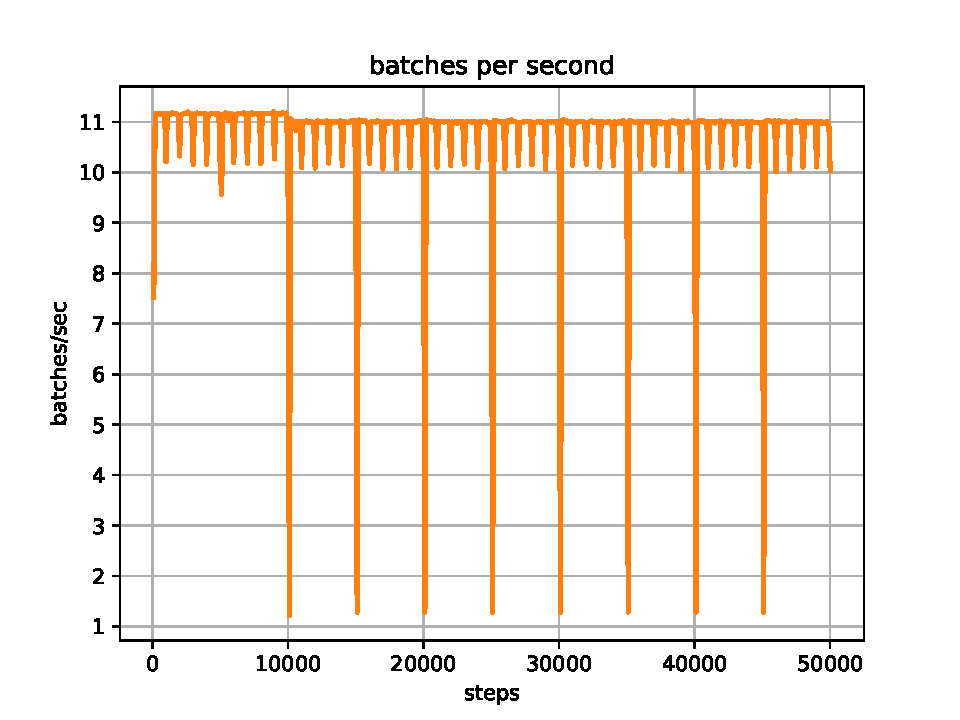
\includegraphics[width=\textwidth]{figures/experiments/Btrain2_batches_per_sec.pdf}
\caption[Οι συστάδες ανά δευτερόλεπτο στο PASCAL\_VOC]{Οι συστάδες ανά δευτερόλεπτο που επεξεργάζεται το δίκτυο κατά την εκπαίδευση στο PASCAL\_VOC. Η τιμή $11$ δηλώνει ότι σε ένα δευτερόλεπτο γίνεται εκπαίδευση σε 220 εικόνες μεγέθους $(334, 500)$.}
\label{fig:pascal_batches_per_sec}
\end{figure}

\begin{figure}
\centering
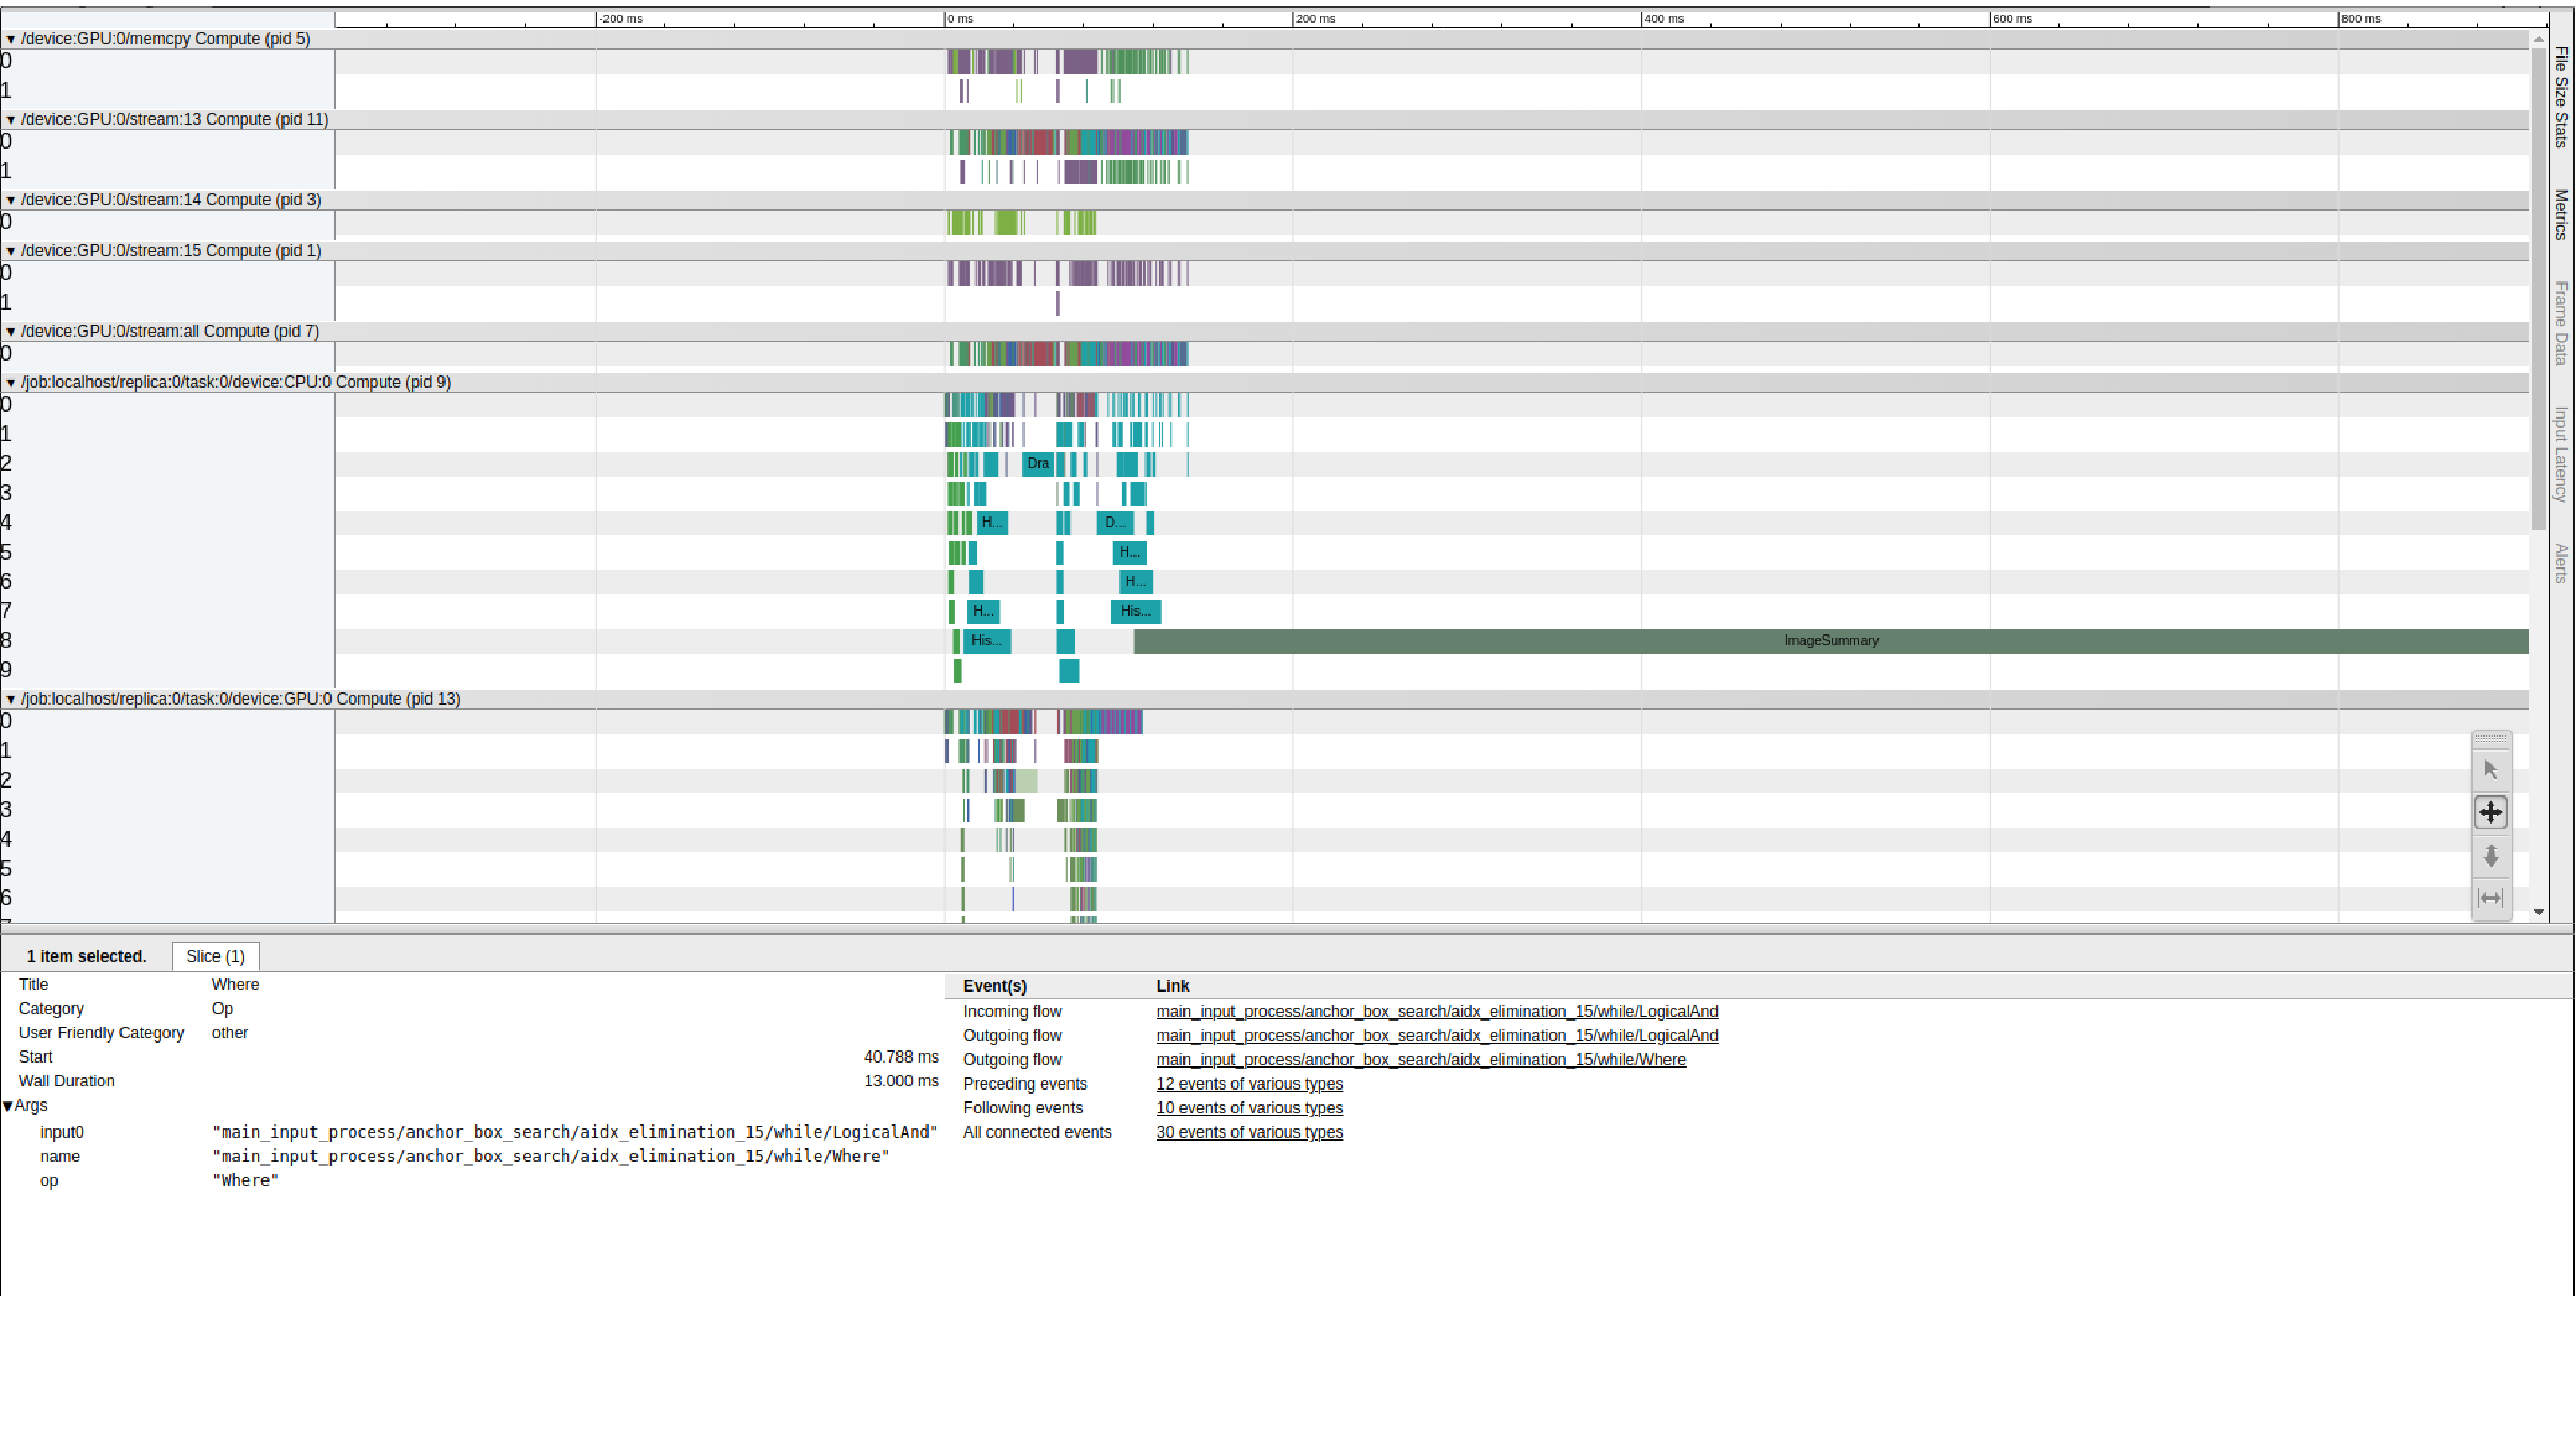
\includegraphics[width=\textwidth]{figures/experiments/pascal_voc_tracing.pdf}
\caption[Χρόνοι εκτέλεσης κάθε επιπέδου στο PASCAL\_VOC]{Οι χρόνοι εκτέλεσης ανά επίπεδο στο PASCAL\_VOC δείχνουν ότι πέρα από τη διαδικασία καταγραφής των στατιστικών εκπαίδευσης η οποία συμβαίνει μία φορά κάθε χίλια βήματα, το πιο αργό επίπεδο είναι στην εύρεση των aidx. Ωστόσο, η συνολική διαδικασία φαίνεται αρκετά επιταχυνόμενη και συμπαγής. Οι μεγάλες κατακόρυφες γραμμές οφείλονται στο κομμάτι οπτικοποίησης του υπολογιστικού γράφου. Τέλος, για περισσότερες λεπτομέρειες τα δεδομένα είναι προσβάσιμα \textcolor{blue}{\href{https://drive.google.com/open?id=1M0m9nAsWXgn3K-tmZxeQARKTLJoRiH2s}{εδώ}} με τη βοήθεια του προγράμματος \textit{"chrome://tracing"}.}
\label{fig:pascal_tracing}
\end{figure}

Προκειμένου να γίνει κατανοητό το πόσο επηρεάζεται συνολικά η χρήση της GPU από τα παραπάνω βήματα μελετήθηκε η κατανάλωση ενέργειας της GPU κατά την εκπαίδευση για 20 λεπτά κατά τη διάρκεια της εκπαίδευσης. Η διαφορά κατανάλωσης στις δύο υλοποιήσεις παρουσιάζεται στο Σχήμα \ref{fig:powerCompare}.

\begin{figure}
    \centering
    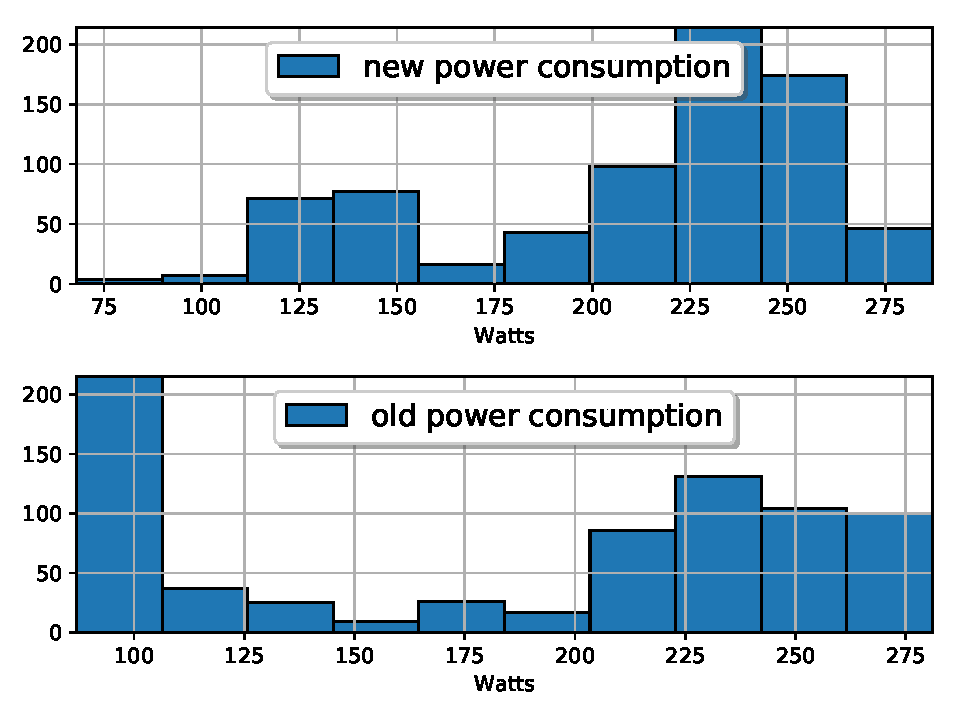
\includegraphics[width=\textwidth]{figures/experiments/power_compare.pdf}
    \caption[Σύγκριση κατανάλωσης ισχύος GPU στις δύο υλοποιήσεις]{Η σύγκριση κατανάλωσης ισχύος GPU στις δύο υλοποιήσεις. Όπως φαίνεται η καινούρια υλοποίηση χρησιμοποιεί περισσότερη ισχύ από ότι η αρχική. Αυτό σημαίνει ότι χρησιμοποιείται πιο πολύ η GPU, πράγμα λογικό αν αναλογιστεί κανείς τα αποτελέσματα του Σχήματος \ref{fig:loadCompare} και τη λογική με την οποία σχεδιάστηκε η καινούρια υλοποίηση.}
    \label{fig:powerCompare}
\end{figure}


\chapter{Υλικό \& λογισμικό}
\label{chapter:architecture}
% about this chapter ~2 paragraphs
Στο κεφάλαιο αυτό παρουσιάζονται τα βασικά εργαλεία που χρησιμοποιήθηκαν
τόσο για τις υλοποιήσεις όσο και για τα πειράματα. Η αναφορά αυτή γίνεται για τον ερευνητή ο οποίος θέλει να εξετάσει λεπτομέρειες της υλοποίησης. Όλα τα σχετικά αρχεία και ο κώδικας βρίσκεται στο \footnote{\url{https://github.com/supernlogn/SqueezeDetTL}}. Στην ενότητα \ref{section:hardware} παρουσιάζεται το υλικό πάνω στο οποίο βασίστηκε η εργασία, ενώ στην ενότητα \ref{section:software} παρουσιάζεται η δόμηση του λογισμικού και τα εργαλεία που χρησιμοποιήθηκαν.

\section{Περιγραφή του υλικού}
\label{section:hardware}
Η παρούσα διπλωματική έγινε στην υπολογιστική συστοιχία του εργαστηρίου Αρχιτεκτονικής Υπολογιστών και Συστημάτων. Τα κύρια μέρη της συστοιχίας που αφορούν είναι 1) η CPU 2) η GPU 3) RAM και ο σκληρός δίσκος. Για περισσότερες λεπτομέρειες, επειδή σε μελλοντικά πειράματα μπορεί να υπάρχουν επιπλέον παράμετροι υλικού, ολόκληρη η ανάλυση του υλικού της συστοιχίας παρατίθεται σε έναν υπερσύνδεσμο\footnote{\url{https://drive.google.com/file/d/1c7IuY3qEbz3VoLnWaWf4ZrtjjNa5O1Rf/view?usp=sharing}}.

\begin{enumerate}
    \item CPU: Intel(R) Core(TM) i7-7700K CPU @ 4.20GHz \footnote{\url{https://ark.intel.com/products/97129/Intel-Core-i7-7700K-Processor-8M-Cache-up-to-4_50-GHz}}
    \item GPU: NVIDIA GEFORCE GTX 1080 Ti \footnote{\url{https://www.nvidia.com/en-us/geforce/products/10series/geforce-gtx-1080-ti/}}
    \item RAM: $2 \times$ DIMM Synchronous 2400 MHz, 8GiB, 64 bits
    \item hard drive: ATA Disk HDD(για τα σύνολα δεδομένων και τα αποτελέσματα) $+$ ATA Disk SSD (για αποθήκευση του κώδικα) 
\end{enumerate}

\section{Βασικά στοιχεία δόμησης λογισμικού}
\label{section:software}
Σε αυτή την ενότητα παρουσιάζονται τα δύο βασικότερα κομμάτια της δόμησης του λογισμικού και τα πακέτα λογισμικού τρίτων.

\subsection{Περιγραφή της δόμησης}
Τα δομικά στοιχεία της συνολικής υλοποίησης είναι εμπνευσμένα από το σχήμα 24 στο βιβλίο νευρωνικών δικτύων του Haykin \cite{66}. Η εικόνα αυτή διαφοροποιημένη φαίνεται στο Σχήμα \ref{fig:haykin_figure}. Εκεί παρουσιάζεται οπτικά και ο τρόπος λειτουργίας της υλοποίησης. Σύμφωνα με αυτή ορίζονται τα δύο μπλοκ \textit{supervisor} και \textit{hypervisor} τα οποία υλοποιούνται στα ομώνυμα πακέτα. Τα δύο αυτά πακέτα αναλύονται παρακάτω.

\begin{figure}
    \centering
    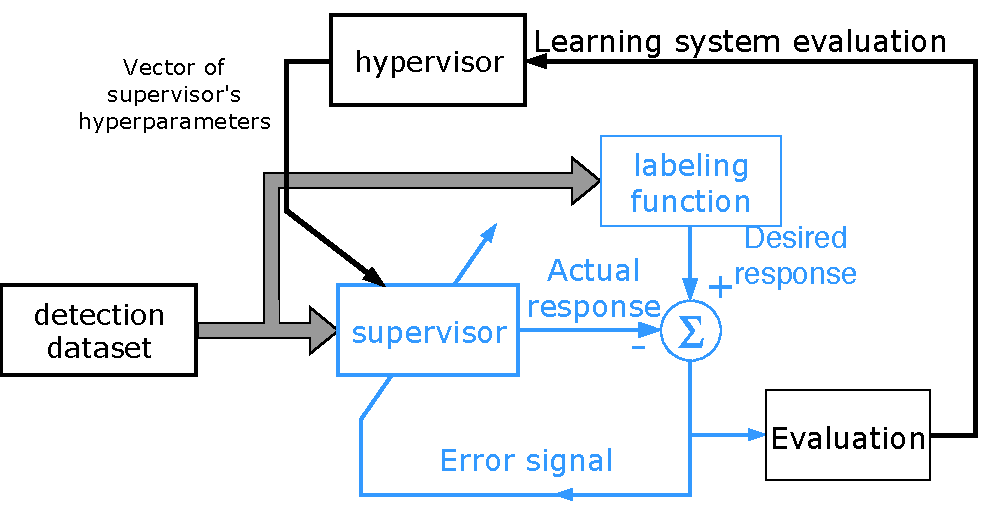
\includegraphics[width = 0.8\textwidth]{figures/architecture/haykin_figure.pdf}
    \caption[Η λειτουργία της υλοποίησης]{Η λειτουργία της υλοποίησης όπως είναι κατά την πορεία της εκπαίδευσης. Ο \textit{supervisor} είναι υπεύθυνος για την εκπαίδευση και βελτιστοποίηση των παραμέτρων του μοντέλου, ενώ ο \textit{hypervisor} είναι υπεύθυνος για τη βελτιστοποίηση των παραμέτρων του \textit{supervisor}.}
    \label{fig:haykin_figure}
\end{figure}

\subsection{supervisor}
Ο \textit{supervisor} είναι υπεύθυνος για την εκπαίδευση του νευρωνικού δικτύου που επιλέγει ο χρήστης. Δηλαδή λαμβάνει ως παραμέτρους το δίκτυο, το σύνολο δεδομένων και όλες τις υπερπαραμέτρους που απαιτούνται κατά την εκπαίδευση από τον \textit{hypervisor} ή τον χρήστη και αναλαμβάνει την συνεχή εκτέλεση του αλγορίθμου back-propagation για το δίκτυο μέχρι αυτό να συγκλίνει στο επιθυμητό οριακό σφάλμα ορισμένο από τον χρήστη ή να αποκλίνει.

Στην πρώτη περίπτωση, επιστρέφονται τα βάρη του δικτύου και ο γράφος της αρχιτεκτονικής του για την ανακατασκευή του. Στη δεύτερη περίπτωση, επιστρέφεται μήνυμα σφάλματος ότι η εκπαίδευση με αυτές τις υπερπαραμέτρους οδηγεί σε αποκλίνουσα συμπεριφορά.

Το σφάλμα το οποίο εξάγεται κατά την διάρκεια της εκπαίδευσης ορίζεται από μία συνάρτηση που αφορά το δίκτυο. Βέβαια, στη παρούσα περίπτωση πρόκειται για την συνάρτηση κόστους του SqueezeDet. Οπότε, δεν αφήνεται περιθώριο για αλλαγές στην εξαγωγή του σφάλματος πέρα από μεταβολή των συντελεστών επιμέρους συντελεστών της συνάρτησης.

Οι υπερπαράμετροι που μπορούν να εισαχθούν για την εκπαίδευση του δικτύου είναι αρκετές. Ωστόσο προκύπτει ότι είναι πιο εύληπτο να εξηγηθούν αυτές, παρά τον πολύπλοκο μηχανισμό που τις υλοποιεί. Παρόλα αυτά, όταν δίνονται οι υπερπαράμετροι σε ένα αρχείο, πιθανόν να περιλαμβάνονται παραπάνω πληροφορίες μέσα στο αρχείο. Οι υπερπαράμετροι που λαμβάνει υπόψιν του το πακέτο \textit{supervisor} είναι οι εξής:

\subsubsection{Λίστα υπερπαραμέτρων}
\begin{itemize}
\setlength{\itemsep}{0pt}
\item \textcolor{LstItemCol}{CLASS\_NAMES} : Τα ονόματα των κλάσεων τα οποία θα κατηγοριοποιηθούν τα εντοπισμένα αντικείμενα.
\item \textcolor{LstItemCol}{CLASSES} : Ο αριθμός των ονομάτων των κλάσεων.
\item \textcolor{LstItemCol}{LEAKY\_COEF} : Παράμετρος διαρροής για τις συναρτήσεις leaky ReLU.
\item \textcolor{LstItemCol}{KEEP\_PROB} : Πιθανότητα να παραμείνει ανεπηρέαστος ένας κόμβος του νευρωνικού δικτύου μετά από εφαρμογή dropout.
\item \textcolor{LstItemCol}{IMAGE\_WIDTH} : Πλάτος εικόνας. Είναι το ίδιο για κάθε εικόνα, αν όχι τότε γίνεται μετατροπή πλάτους της εικόνας εισόδου σε αυτό.
\item \textcolor{LstItemCol}{IMAGE\_HEIGHT} : Ύψος εικόνας. Είναι το ίδιο για κάθε εικόνα, αν όχι τότε γίνεται μετατροπή ύψους της εικόνας εισόδου σε αυτό.
\item \textcolor{LstItemCol}{ANCHOR\_BOX} : Πίνακας ο οποίος εμπεριέχει "anchors" όπως λέγονται στο SqueezeDet \cite{1}, δηλαδή στοιχεία τύπου $(cx,xy,w,h)$, όπου $cx$ η τετμημένη κέντρου του anchor, $cy$ η τεταγμένη κέντρου του anchor, $w$ το πλάτος του anchor και $h$ το ύψος του anchor.
\item \textcolor{LstItemCol}{ANCHORS} : Ο συνολικός αριθμός των anchor
\item \textcolor{LstItemCol}{ANCHOR\_PER\_GRID} : Ο αριθμός των anchor ανά σημείο του τελικού πλέγματος (βλέπε \cite{1}).
\item \textcolor{LstItemCol}{INITIAL\_ANCHOR\_SHAPES} : Πίνακας με προκαθορισμένες τιμές του πλάτους και του ύψους κάθε anchor.
\item \textcolor{LstItemCol}{BATCH\_SIZE} : Μέγεθος της παρτίδας για ευρωστότερη εκπαίδευση, συνίσταται ο αριθμός αυτός να είναι ίσος με 1 για μετεκπαίδευση σε μικρά σετ δεδομένων.
\item \textcolor{LstItemCol}{PROB\_THRESH} : Κατώφλι το οποίο ορίζει αν ένα υποψήφιο εντοπισμένο αντικείμενο θα θεωρηθεί ως ορθό και θα δοθεί ως είσοδο στον αλγόριθμο NMS.
\item \textcolor{LstItemCol}{PLOT\_PROB\_THRESH} : Κατώφλι το οποίο ορίζει αν ένα εντοπισμένο αντικείμενο θα προβληθεί στα αποτελέσματα προς οπτικοποίηση. Χρησιμοποιείται μόνο κατά την οπτικοποίηση των αποτελεσμάτων.
\item \textcolor{LstItemCol}{NMS\_THRESH} : Ανώφλι μετρικής iou μεταξύ των κουτιών που εντοπίστηκαν. Αν δύο κουτιά έχουν μεταξύ τους μεγαλύτερη τιμή iou, τότε κάποιο από αυτά θα αφαιρεθεί όπως προβλέπεται από τον αλγόριθμο NMS.
\item \textcolor{LstItemCol}{TOP\_N\_DETECTION} : Ο μέγιστος αριθμός αντικειμένων τα οποία θα εξαχθούν από μία εικόνα στο πέρα του αλγορίθμου του νευρωνικού δικτύου.
\item \textcolor{LstItemCol}{BGR\_MEANS} : Μέση τιμή του χρώματος των pixel στο σετ δεδομένων σε σειρά BGR ως ένας πίνακας (1, 1, 3).
\item \textcolor{LstItemCol}{LOSS\_COEF\_CONF} : Συντελεστής σφάλματος εμπιστοσύνης παλινδρόμησης.
\item \textcolor{LstItemCol}{LOSS\_COEF\_CLASS} : Συντελεστής σφάλματος παλινδρόμησης της κατηγοριοποίησης.
\item \textcolor{LstItemCol}{LOSS\_COEF\_BBOX} : Συντελεστής σφάλματος παλινδρόμησης του περιβλήματος των υποψήφιων εντοπισμένων αντικειμένων.
\item \textcolor{LstItemCol}{LOSS\_COEF\_CONF\_POS} : Συντελεστής θετικού σφάλματος εμπιστοσύνης για τη παλινδρόμηση του σκορ.
\item \textcolor{LstItemCol}{LOSS\_COEF\_CONF\_NEG} : Συντελεστής αρνητικού σφάλματος εμπιστοσύνης για τη παλινδρόμηση του σκορ. 
\item \textcolor{LstItemCol}{DECAY\_STEPS} : Άριθμος βημάτων κατά τον οποίο γίνεται σμίκρυνση του ρυθμού ανανέωσης βαρών.
\item \textcolor{LstItemCol}{LR\_DECAY\_FACTOR} : Αριθμός με τον οποίο πολλαπλασιάζεται ο ρυθμός μάθησης κάθε \textcolor{LstItemCol}{DECAY\_STEPS} επαναλήψεις.
\item \textcolor{LstItemCol}{LEARNING\_RATE} : Αρχικός ρυθμός μάθησης(ανανέωσης βαρών).
\item \textcolor{LstItemCol}{MOMENTUM} : Ορμή, Χρησιμοποιείται για τον βελτιστοποιητή ορμής \cite{42}.
\item \textcolor{LstItemCol}{BETA1} : Παράμετρος του βελτιστοποιητή Adam beta1.
\item \textcolor{LstItemCol}{BETA2} : Παράμετρος του βελτιστοποιητή Adam beta2.
\item \textcolor{LstItemCol}{WEIGHT\_DECAY} : ποσοστό μείωσης της τιμής του μέτρου των παραμέτρων κατά την ανανέωση τους σε κάθε επανάληψη.
\item \textcolor{LstItemCol}{LOAD\_PRETRAINED\_MODEL} : Αν τα βάρη θα αρχικοποιηθούν όπως στο \cite{1}.
\item \textcolor{LstItemCol}{PRETRAINED\_MODEL\_PATH} : Διαδρομή αρχείου για την αρχικοποίηση του αρχείου. Πρόκειται για αρχείο τύπου \textit{pkl}.
\item \textcolor{LstItemCol}{DEBUG\_MODE} : Ενεργοποίηση ή όχι της λειτουργίας αποσφαλμάτωσης.
\item \textcolor{LstItemCol}{EPSILON} : Πολύ μικρή τιμή για να αποτραπεί η αριθμητική αστάθεια στις πράξεις.
\item \textcolor{LstItemCol}{EXP\_THRESH} : Ανώφλι για τις ασφαλείς εκθετικές συναρτήσεις.
\item \textcolor{LstItemCol}{MAX\_GRAD\_NORM} : Ανώφλι μέτρου παραγώγων. Παράγωγοι με τιμή μεγαλύτερη δε λαμβάνονται υπόψη.
\item \textcolor{LstItemCol}{DATA\_AUGMENTATION} : Αν θα γίνει προσαύξηση των δεδομένων με πρόσθεση θορύβου.
\item \textcolor{LstItemCol}{EXCLUDE\_HARD\_EXAMPLES} : Υπερπαράμετρος που αφορά το σύνολο δεδομένων KITTI.
\item \textcolor{LstItemCol}{BATCH\_NORM\_EPSILON} : Μικρή τιμή που χρησιμοποιείται στους παρονομαστές για τις διαιρέσεις που απαιτεί η εκπαίδευση κατά παρτίδες. Η προκαθορισμένη τιμή είναι αυτή που χρησιμοποιεί και το Caffe framework \cite{101}.
\item \textcolor{LstItemCol}{FREEZE\_LAYERS} : Αντικείμενο που ορίζει για κάθε επίπεδο του νευρωνικού αν θα εκπαιδευτεί ή όχι.
\item \textcolor{LstItemCol}{IS\_TRAINING} : Αν πρόκειται για εκπαίδευση(true) ή απλά για εκτίμηση του μοντέλου(false).
\item \textcolor{LstItemCol}{NUM\_THREAD} : Αριθμός των νημάτων τα οποία εξάγουν δεδομένα από το σετ δεδομένων.
\item \textcolor{LstItemCol}{MAX\_NUM\_PARALLEL\_NETS} : Μέγιστος αριθμός παράλληλων εκπαιδεύσεων.
\item \textcolor{LstItemCol}{PREPROCESS\_DATASET} : Η αληθής τιμή αυτής της υπερπαραμέτρου επιτρέπει την προ-επεξεργασία όλου του σετ δεδομένων και την εξαγωγή των μεταβλητών aidx και deltas για γρηγορότερη εκπαίδευση αργότερα. Ωστόσο, αν η προ-επεξεργασία ενεργοποιηθεί δεν επιτρέπει μοντέλα με διαφορετική αρχιτεκτονική στο επίπεδο που εξάγονται τα anchor.
\end{itemize}

Τέλος, ο υπολογιστικός γράφος του νευρωνικού δικτύου εντοπισμού με βάση αυτή την υλοποίηση φαίνεται στο Σχήμα \ref{fig:computation_graph} στο τέλος του κεφαλαίου. Εκεί γίνονται εμφανείς και περισσότερες λεπτομέρειες της υλοποίησης.

\subsection{hypervisor}
Το πακέτο αυτό είναι υπεύθυνο για το χειρισμό των υπερπαραμέτρων. Στο κύριο μέρος του υλοποιεί έναν αλγόριθμο βελτιστοποίησης μαύρου κουτιού όπως αυτός που περιγράφεται στην ενότητα \ref{section:autohyperparamters}. Αν και στην προαναφερόμενη ενότητα υλοποιείται μόνο ένας από αυτούς, υπάρχει η δυνατότητα επιλογής μεταξύ τεσσάρων αλγορίθμων όπως περιγράφονται στην παρακάτω λίστα.
\begin{enumerate}
    \item random search: Τυχαία αναζήτηση η οποία δοκιμάζει κάθε φορά καινούριες τυχαίες τιμές ως τιμές των παραμέτρων, παραγόμενες από μία γεννήτρια τυχαίων αριθμών.
    \item LIPO: Ο πρώτος αλγόριθμος που παρουσιάζεται στην εργασία του Nicolas και του Cedric \cite{64}. Οι σταθερές $k$ που χρησιμοποιούνται είναι 1, 10, 100. Επίσης ορίζεται μέγιστος αριθμός επαναλήψεων ίσος με 50.
    \item adaLIPO: Ο δεύτερος αλγόριθμος που παρουσιάζεται στην ίδια εργασία. Στη μόνη ρύθμιση που αρκείται είναι στο μέγιστο αριθμό επαναλήψεων (ίσος με 50).
    \item genetic: Ένας τυπικός γενετικός αλγόριθμος σύμφωνα με τις προτάσεις στο \cite{69}. Οι ρυθμίσεις του είναι δίνονται από τον χρήστη.
\end{enumerate}

Την τιμή εκκίνησης και την περιοχή(πλέγμα) στην οποία γίνεται η αναζήτηση της βέλτιστης τιμής των υπερπαραμέτρων την βάζει ο χρήστης για κάθε αλγόριθμο βελτιστοποίησης. Όπως επίσης, εισάγει και τις τιμές ρύθμισης τους αν αυτές απαιτούνται. Εδώ να τονιστεί πως αυτό δεν χρειάζεται για τον αλγόριθμο \textit{adalipo}, αυτό είναι και ένα από τα πλεονεκτήματά του.

Το πακέτο \textit{hypervisor} λαμβάνει ως τιμές τις συνάρτησης βελτιστοποίησης την έξοδο(κύρια μετρική) της διαδικασίας εκτίμησης του μοντέλου. Η μετρική που μελετάται στη συγκεκριμένη περίπτωση είναι η mAP. Η προτίμηση αυτή γίνεται για την καλύτερη σύνδεση με την πρωταρχική εργασία του \textit{SqueezeDet}.

Αν και υπάρχει πληθώρα άλλων πακέτων για αυτή την υλοποίηση, ωστόσο τα υπόλοιπα δεν παρουσιάζονται διότι δεν έχουν μεγάλη σημασία.

\subsection{Περιγραφή πακέτων λογισμικού τρίτων}
Η γλώσσα προγραμματισμού που χρησιμοποιήθηκε ήταν η Python 2.7, διότι είναι πιο πλήρως υποστηριζόμενη από το \textit{Tensorflow}(βλέπε παρακάτω). Το λειτουργικό της συστοιχίας ήταν \textit{Ubuntu 16.04.4 LTS (Xenial Xerus)}. Τα πακέτα που χρησιμοποιήθηκαν στη τελική υλοποίηση δεν ήταν πολλά γιατί όλες οι υπολογιστικές ανάγκες αυτής της εργασίας καλυπτόταν από τις βιβλιοθήκες \textit{Tensorflow} και \textit{NumPy}.

\begin{itemize}
    \item Tensorflow\footnote{\url{https://www.tensorflow.org}} \cite{34}: Ανοικτού κώδικα βιβλιοθήκη για αριθμητικούς υπολογισμούς χρησιμοποιώντας γράφους ροής δεδομένων ανεπτυγμένο από την ερευνητική ομάδα της \textit{Google}. Η ευέλικτη αρχιτεκτονική της επιτρέπει την ανάπτυξη λογισμικού σε μία ή και περισσότερες κεντρικές μονάδες επεξεργασίας CPU ή μονάδες GPU ακόμα και για ενσωματωμένες συσκευές.
    \item NumPy\footnote{\url{http://www.numpy.org}}: Το βασικό πακέτο για επιστημονικούς υπολογισμούς στην Python. Η χρήση του βοήθησε κυρίως στην υλοποίηση του hypervisor, διότι αυτός εκτελείται από τη CPU.
    \item Matplotlib\footnote{\url{https://matplotlib.org/}}: Βιβλιοθήκη της Python για κατασκευή διαγραμμάτων.
    \item Google-Protocol-buffers(protoc)\footnote{\url{https://developers.google.com/protocol-buffers}}: Επεκτάσιμος μηχανισμός της Google για τη σειριοποίηση δομημένων δεδομένων. Ο μηχανισμός αυτός είναι ανεξάρτητος πλατφόρμας, είναι παρόμοιος με αυτόν της XML, ωστόσο μικρότερος και γρηγορότερος. Η κάθε ανάγνωση και συγγραφή γίνεται με συναρτήσεις οι οποίες έχουν παραχθεί από τον μηχανισμό αυτό ειδικά για κάθε περίπτωση. 
    \item vod-converter\footnote{\url{https://github.com/umautobots/vod-converter}}: Εργαλείο για την μετατροπή της μορφής των συνόλων δεδομένων KITTI, PASCAL VOC από το ένα σύνολο δεδομένων στο άλλο. Η παρούσα εργασία συνείσφερε και στην ανάπτυξη αυτού του εργαλείου, πέρα από την χρήση του.
    \item dlib \footnote{\url{http://dlib.net/}} \cite{83}: Βιβλιοθήκη μεθόδων μη γραμμικής βελτιστοποίησης στη C++. Η χρήσης της βοήθησε στην ανάπτυξη και την βελτιστοποίηση της μεθόδου που περιγράφεται στην ενότητα \ref{section:autohyperparamters}.
\end{itemize}

\begin{figure}
    \centering
    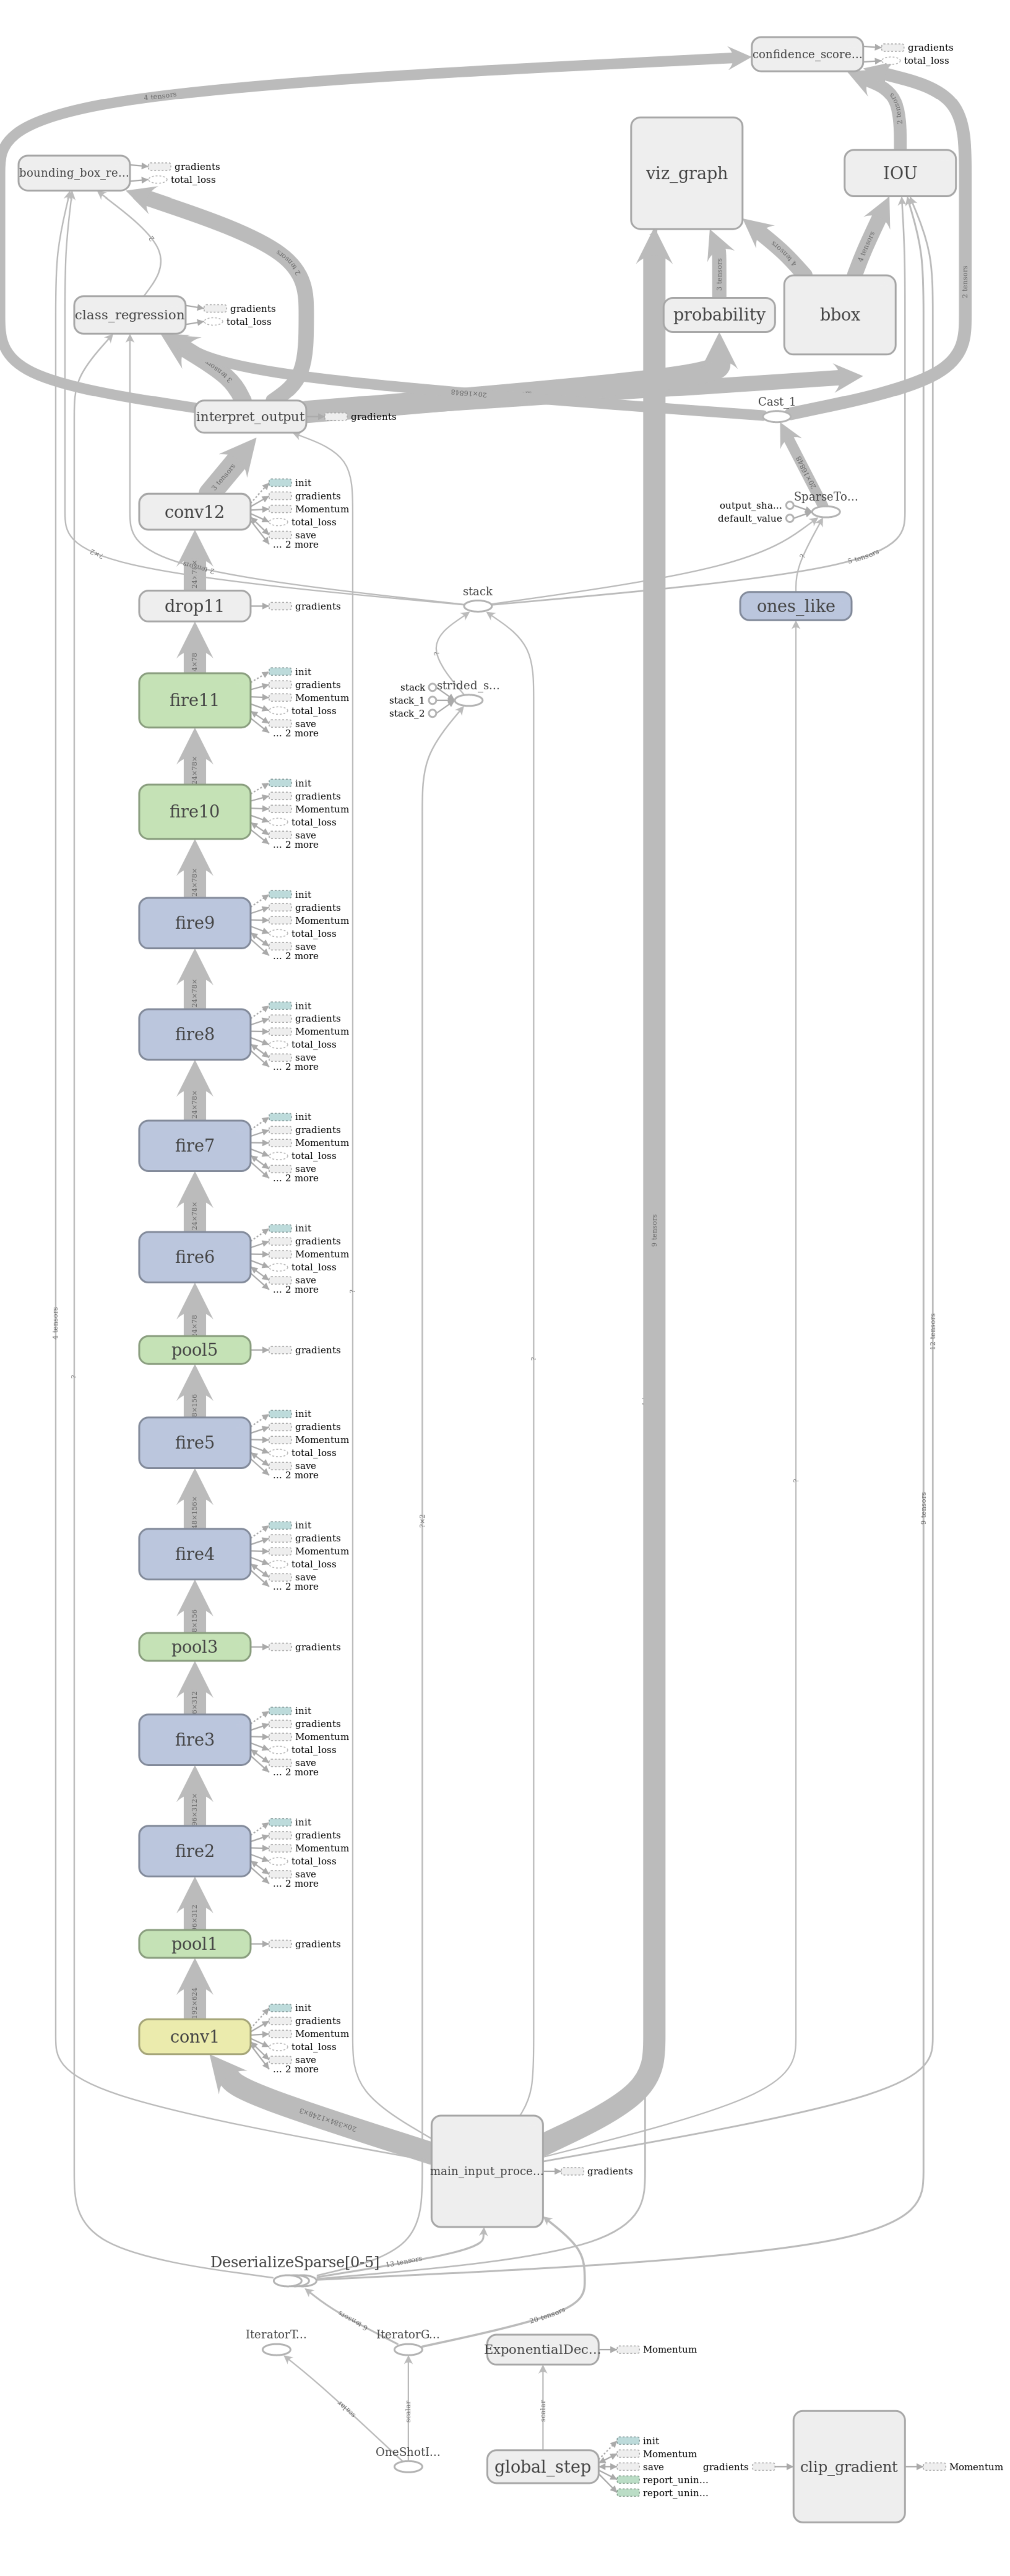
\includegraphics[width=\textwidth,height=\textheight]{figures/architecture/comp_graph.pdf}
    \caption[Ο υπολογιστικός γράφος της υλοποίησης]{Ο υπολογιστικός γράφος της υλοποίησης του SqueezeDet. Το κάθε κομμάτι του γράφου υλοποιεί έναν υπολογισμό. Η πληθώρα αυτών των κομματιών βρίσκεται τοποθετημένη στην GPU. Τα κομμάτια που δεν βρίσκονται στη GPU αφορούν κυρίως την ανάγνωση των δεδομένων από τον δίσκο.}
    \label{fig:computation_graph}
\end{figure} % DONE
\chapter{Μελλοντικές επεκτάσεις}
\label{chapter:futures}
Είναι σημαντικό να ερευνηθεί η εκτέλεση του πειράματος της ενότητας \ref{section:catastrophicForgetting}, ώστε να μπορέσει να εξετασθεί αν έχει νόημα η δημιουργία του γράφου στο Σχήμα \ref{fig:transferability_graph}, όπως επίσης και συστήματα που λειτουργούν κατά αυτό τον τρόπο. Όπως υποδεικνύει η βιολογία του εγκεφάλου τέτοια συστήματα εξυπηρετούν κατά πολύ στην χρήση ελάχιστων νευρώνων και την γρήγορη μάθηση καινούριων αντικειμένων. Όπως επίσης έχει υποδείξει και ο Hinton \cite{79} ο αριθμός των νευρώνων των νευρωνικών δικτύων επεξεργασίας εικόνας είναι κατά πολύ μεγαλύτερος από ότι χρειάζεται, όπως επίσης δεν χρειάζεται ενεργοποίηση όλων των νευρώνων για κάθε αντικείμενο. Για αυτό κρίνεται απαραίτητη η εξέταση της πλαστικότητας των νευρώνων ως προς την επανεκπαίδευση στις αρχιτεκτονικές νευρωνικών δικτύων με μικρό αριθμό νευρώνων.

Τα συστήματα που προτείνονται προς μελλοντική εξέταση είναι το MobileNet \cite{77} με το SSD, μία αρχιτεκτονική η οποία αναπτύχθηκε κατά τη διάρκεια εκπόνησης αυτής της εργασίας. Όπως επίσης, κρίνεται σκόπιμο να διερευνηθεί αν τα υπόλοιπα δίκτυα που σχετίζονται με το SqueezeDet, όπως το SqueezeDet+, VGG16 + ConvDet και ResNet50 + ConvDet, τα οποία αναφέρονται στο \cite{1}, έχουν την ίδια συμπεριφορά. Επίσης, επειδή ένας άλλος μεγάλος ανταγωνιστής του SqueezeDet είναι το YOLO (εξετάστηκε στο κεφάλαιο \ref{chapter:neuralNets}), προτείνεται και η διερεύνηση της μεταφαρσιμότητας και της πλαστικότητας των νευρώνων και αυτού του δικτύου.

Επιπλέον, λόγω πολλών ωρών εκτέλεσης της εκπαίδευσης δεν μπόρεσε να γίνει στα πλαίσια της διαθέσιμης τεχνολογίας και των εβδομάδων που διατίθενται σε μία διπλωματική εργασία η πλήρης εξερεύνηση της επίδοσης του αλγορίθμου στο χώρο των υπερπαραμέτρων. Ένα ολοκληρωμένων πείραμα με τη χρήση μόνο μίας εκ των μεθόδων υπολογίστηκε πως απαιτεί στην υπολογιστική συστοιχία του εργαστηρίου (\ref{section:hardware}) ~80 εβδομάδες. Οπότε, όταν βρεθούν οι κατάλληλοι πόροι για ικανό χρόνο θα ήταν σημαντική εξέταση για να δείξει αν υπάρχει βελτίωση/διατήρηση της συμπεριφοράς όχι μόνο στο παρόν πείραμα με το SqueezeDet αλλά και σε αυτό που βασίστηκε \cite{55}.

Αυτή η διπλωματική ξεκίνησε με σκοπό την αυτοματοποίηση της μετάδοσης γνώσης σε αλγορίθμους εντοπισμού αντικειμένων πραγματικού χρόνου και τη γρήγορη μετεκπαίδευση σε καινούρια σύνολα δεδομένων για την αποστολή παραμέτρων εντοπισμού αντικειμένων. Ωστόσο, προκειμένου να είναι εφικτός ο αυτοματισμός θα έπρεπε πρώτα να είναι γνωστή η συμπεριφορά του αλγορίθμου που θα χρησιμοποιόταν σε αυτό το σύστημα ως προς τη μεταφερσιμότητα των παραμέτρων του. Πλέον, αυτή είναι γνωστή για το SqueezeDet, οπότε και είναι δυνατή η κατασκευή αυτοματοποιημένου συστήματος μετάδοσης γνώσης βασιζόμενο σε αυτό. 

Μία ακόμα ενδιαφέρουσα προοπτική είναι η ανάπτυξη αυτού του συστήματος στο \textit{cloud} με το οποίο θα μπορούσαν να επικοινωνούν απευθείας όλες οι ενσωματωμένες συσκευές. Σε μία τέτοια προσπάθεια αν επιπλέον σχεδιάζεται να ενταχθούν περισσότερα δίκτυα/αλγόριθμοι, θα ήταν θεμιτή η ένταξη των αλγορίθμων σε ένα σύστημα όπως το Tensorflow Object Detection API\footnote{\url{https://github.com/tensorflow/models/tree/master/research/object_detection}} της \textit{Google}, το οποίο σκοπεύει στην υλοποίηση του ίδιου ακριβώς συστήματος, ωστόσο με αυτοματοποιημένο μόνο το κομμάτι της εκπαίδευση και όχι της επιλογής των υπερπαραμέτρων. Επίσης, μπορούν να ληφθούν υπόψη οι χρόνοι από την εκτέλεση του πειράματος στην ενότητα \ref{section:grantExpRes} για καλύτερη διαχείρηση του συστήματος. % Not started yet
\include{JStry}
% \chapter{Μηχανισμός μεταφοράς παραμέτρων}


\section{Περιληπτική ανάλυση του μηχανισμού}
Ο μηχανισμός που υλοποιήθηκε για αυτή την εργασία αποτελείται από δύο σκέλη. Το πρώτο αφορά την υπηρεσία που βρίσκεται στον server και αφορά την εκπαίδευση και επανεκπαίδευση νευρωνικών δικτύων. Στη μεριά του server όπως είναι φυσικό, το σύστημα έχει περισσότερους υπολογιστικούς πόρους, οπότε και το λογισμικό μπορεί να γραφεί σε πιο υψηλό επίπεδο. Το δεύτερο σκέλος αφορά το λογισμικό από πλευράς του ρομποτικού πράκτορα. Όπως είναι κατανοητό αυτό βρίσκεται σε ενσωματωμένη συσκευή και δεν έχει πολλούς υπολογιστικούς πόρους. Για αυτό και προσπαθούμε να μεταφέρουμε τον φόρτο εργασίας όσο περισσότερο γίνεται στην μεριά του server. Βέβαια να τονισθεί σε αυτό το σημείο πως αν οι ρομποτικοί πράκτορες γίνουν περισσότεροι και αυξηθούν οι υπολογιστικοί πόροι τους, τότε θα πρέπει να υπάρξει και μία συνεργασία, ώστε να ελαφρυνθεί υπολογιστικά ο server.

Στο κομμάτι του server ο χρήστης είναι ένας ρομποτικός πράκτορα για αυτό και μέσα στα διαγράμματα σημειώνεται ως \textit{robot}. Βέβαια αυτός ο χρήστης μπορεί να είναι και η εφαρμογή στο κινητό τηλέφωνο ενός ανθρώπου. Ωστόσο, για να διατηρηθεί η παρουσίαση της γενικότητας του μηχανισμού υποθέτουμε ένα πιο αφηρημένο είδος χρήστη.

Αντίστοιχα, στο κομμάτι του ρομποτικού πράκτορα / ενσωματωμένης συσκευής ο server μετ-εκπαίδευσης των βαρών θεωρείται ως εξωτερικό σύστημα. Αυτό επιτρέπει την ανάλυση και την υλοποίηση του συστήματος σε δύο ανεξάρτητα μέρη.

\section{Απαιτήσεις μηχανισμού μεταφοράς παραμέτρων}
Ο μηχανισμός μεταφοράς παραμέτρων στο στάδιο αυτής της εργασίας έχει λίγες απαιτήσεις σε αριθμό, διότι η κάθε μία από αυτές απαιτεί χρόνο όσον αφορά την ανάπτυξη της λύσης. Οι απαιτήσεις αφορούν μόνο τη μεταφορά παραμέτρων του νευρωνικού δικτύου SqueezeDet+ από τον server(σύστημα) προς τον ρομποτικό πράκτορα.

\begin{enumerate}
    \item Ο ρομποτικός πράκτορας πρέπει να μπορεί να αναζητήσει παραμέτρους εντοπισμού ενός σετ αντικειμένων που υπάρχουν στο σύστημα.
    \item Ο ρομποτικός πράκτορας πρέπει να μπορεί να απαιτήσεις τη δημιουργία παραμέτρων εντοπισμού ενός σετ αντικειμένων από το σύστημα.
    \item Ο ρομποτικός πράκτορας πρέπει να μπορεί να λάβει παραμέτρους εντοπισμού ενός σετ αντικειμένων που υπάρχουν στον server.
    \item Ο ρομποτικός πράκτορας πρέπει να μπορεί να ενημερώνεται για την κατάσταση στην οποία βρίσκεται η εκπαίδευση παραμέτρων ενός σετ αντικειμένων.
    \item Ο ρομποτικός πράκτορας πρέπει να μπορεί να λάβει την αρχιτεκτονική του νευρωνικού δικτύου εντοπισμού και τις απαραίτητες παραμέτρους για την κατασκευή του.
\end{enumerate}
 
Οι παραπάνω λειτουργικές απαιτήσεις αφορούν το βασικό στάδιο του λογισμικού και συνδέονται με τις παρακάτω μη λειτουργικές απαιτήσεις.
\begin{enumerate}
    \item Η επικοινωνία με τον ρομποτικό πράκτορα θα έπρεπε να γίνεται μέσω πρωτοκόλλου \textit{TCP/IP}.
    \item Η επικοινωνία με τον ρομποτικό πράκτορα θα έπρεπε να απαιτεί τη μεταφορά του μικρότερου δυνατού όγκου δεδομένων.
\end{enumerate}

Αυτές οι μη λειτουργικές απαιτήσεις ουσιαστικά θέτουν το πλαίσιο μέσα στο οποίο θα υλοποιηθεί η επικοινωνία και οι κλήσεις μεταξύ συστήματος και ρομποτικού πράκτορα. Συνολικά παρατηρείται ότι οι απαιτήσεις είναι ελάχιστες. Ωστόσο, δε θα μπορούσε να είναι περισσότερες διότι αυτές θέτουν τη βάση για μία ορθή και βάσιμη υλοποίηση που θα μπορεί να δεχθεί επέκταση μετέπειτα. Οποιεσδήποτε επιπλέον απαιτήσεις προστίθενται και στα αντίστοιχα κεφάλαια. Στο τέλος της εργασίας δίνεται μία πλήρη λίστα αυτών.

\section{Αρχιτεκτονική μηχανισμού μεταφοράς παραμέτρων}
\subsection{Εισαγωγικά}
Η αρχιτεκτονική του μηχανισμού μεταφοράς παραμέτρων ακολουθεί σαν βάση την αρχιτεκτονική που χρησιμοποιείται από ερευνητές για την δημιουργία καινούριων νευρωνικών δικτύων και για τον ολικό έλεγχό τους. Η προσέγγιση και το σκεπτικό που ακολουθήθηκε στην σχεδίαση ήταν ο διαχωρισμός των κομματιών που πράττουν διαφορετικό έργο κατά το δυνατό περισσότερο. Επίσης, όλες οι παράμετροι που χρησιμοποιούνται στο σύστημα να δίνονται ως ξεχωριστή είσοδος από αρχεία και σε αυτές τις παραμέτρους να ξεχωρίζουν αυτές που είναι \textbf{α}) μεταβαλλόμενες από το σύστημα \textbf{β}) μεταβαλλόμενες από τον ρομποτικό πράκτορα \textbf{γ}) σταθερές.

Επίσης χρησιμοποιείται και μία αρχιτεκτονική αρχείων για την αποθήκευση των παραμέτρων για εντοπισμό κάθε σετ αντικειμένων. Αν και θα μπορούσε να χρησιμοποιηθεί μία βάση δεδομένων, προτιμήθηκε να χρησιμοποιηθεί ένα αρχείο ευρετηρίου και το σύστημα αρχείων που ήδη έχει το εκάστοτε λειτουργικό, για καλύτερη συμβατότητα με τα σετ εκπαίδευσης.

\subsection{Τεχνολογίες και πακέτα χρήσης}
Το βασικότερο που πρέπει να τονιστεί σε αυτό το σημείο είναι πως η πλατφόρμα από μεριάς του server βασίστηκε σε λειτουργικό Linux Ubuntu 14.04, δεν ελέγχθηκε η λειτουργία σε κάποιο άλλο λειτουργικό. Επίσης η αρχιτεκτονική έχει αυτή τη μορφή εκτός από το συνολικό σκεπτικό και λόγω τριών αποφάσεων
\begin{itemize}
    \item της γλώσσας υλοποίησης που επιλέχθηκε (Python 2.7),
    \item της αρχιτεκτονικής της βιβλιοθήκης δημιουργίας νευρωνικών δικτύων TensorFlow (1.7)[???]
    \item της μορφής του σετ εκπαίδευσης ενός από τα pascal\_voc, ms_coco, google openImages.
    \item και της αρχιτεκτονικής REST εξυπηρέτησης αιτημάτων του ρομποτικού πράκτορα.
\end{itemize}



Η βιβλιοθήκη TensorFlow[???]:

Το σετ δεδομένων pascal\_voc[???]

\definecolor{mygreenii}{RGB}{124,166,198}
\definecolor{mygreeni}{RGB}{110,144,169}

\begin{forest}
  for tree={
    font=\sffamily,
    text=white,
    text width=2cm,
    minimum height=0.75cm,
    if level=0
      {fill=mygreenii}
      {fill=mygreeni},
    rounded corners=4pt,
    grow'=0,
    child anchor=west,
    parent anchor=south,
    anchor=west,
    calign=first,
    edge={mygreenii,rounded corners,line width=1pt},
    edge path={
      \noexpand\path [draw, \forestoption{edge}]
      (!u.south west) +(7.5pt,0) |- (.child anchor)\forestoption{edge label};
    },
    before typesetting nodes={
      if n=1
        {insert before={[,phantom]}}
        {}
    },
    fit=band,
    s sep=15pt,
    before computing xy={l=15pt},
  }
[text1
  [text1.1
    [text1.1.1]
    [text1.1.2]
    [text1.1.3]
  ]
  [text1.2
    [text1.2.1]
    [text1.2.2]
  ]
]
\end{forest}

Η αρχιτεκτονική REST[???, ???]



\subsection{Διάγραμμα πακέτων και κλάσεων}



\section{Υλοποίηση σε πλατφόρμες}

\subsection{Βελτιστοποιήσεις}

\section{Πειραματικά αποτελέσματα}
% \chapter{Εκπαίδευση \& Επαν-εκπαίδευση με ανεξαρτησία θορύβου γραμμικού μετασχηματισμού}
% \chapter{Παράρτημα}

Σε αυτό το κομμάτι της εργασίας παρατίθενται γνώσεις που πιθανόν να χρειαστεί ο αναγνώστης πριν την ανάγνωση των υπολοίπων κεφαλαίων. Φυσικά, αυτή δεν είναι πλήρης για αυτό παραπέμπεται στη βιβλιογραφία αυτού του κεφαλαίου αν ο ίδιος θέλει να την κατανοήσει σε βάθος.


\section{Νευρωνικά Δίκτυα}


\subsection{Αρχιτεκτονικές}

\subsection{Τρόποι εκπαίδευσης}


\section{Στοιχεία Ψηφιακής Επεξεργασίας Εικόνας}


\section{Στοιχεία Ανάλυσης Τανυστών και Πολλαπλοτήτων}





% \bibliographystyle{hellas}
\printbibliography


\end{document}
